\chapter{Results}
\label{ch:results}

This Chapter presents the results of the analysis described in the previous chapter. 
Comparing the results of 30 and 50 seasons per timescope revealed (similar to \cite{vietinghoff_visual_2021}) that using 30 winters is in general more noisy, but the results are structurally very similar. 
Therefore, only the more smooth results of 50 winters per timescope are shown in this section, while some of the results of 30 seasons can be found in the Appendix for comparison. 

\section{Evolution of Patterns}
\label{sec:pattern evolution}

This Section gives an overview how the EOF patterns change over the time, also comparing the differences of the two chosen climate scenarios, which represent the extremes of climate change handling.   

\subsection{Evolution of Encoded Variability}
\label{sec:results encoded variance}



\begin{figure}[htb]
  \begin{center}
    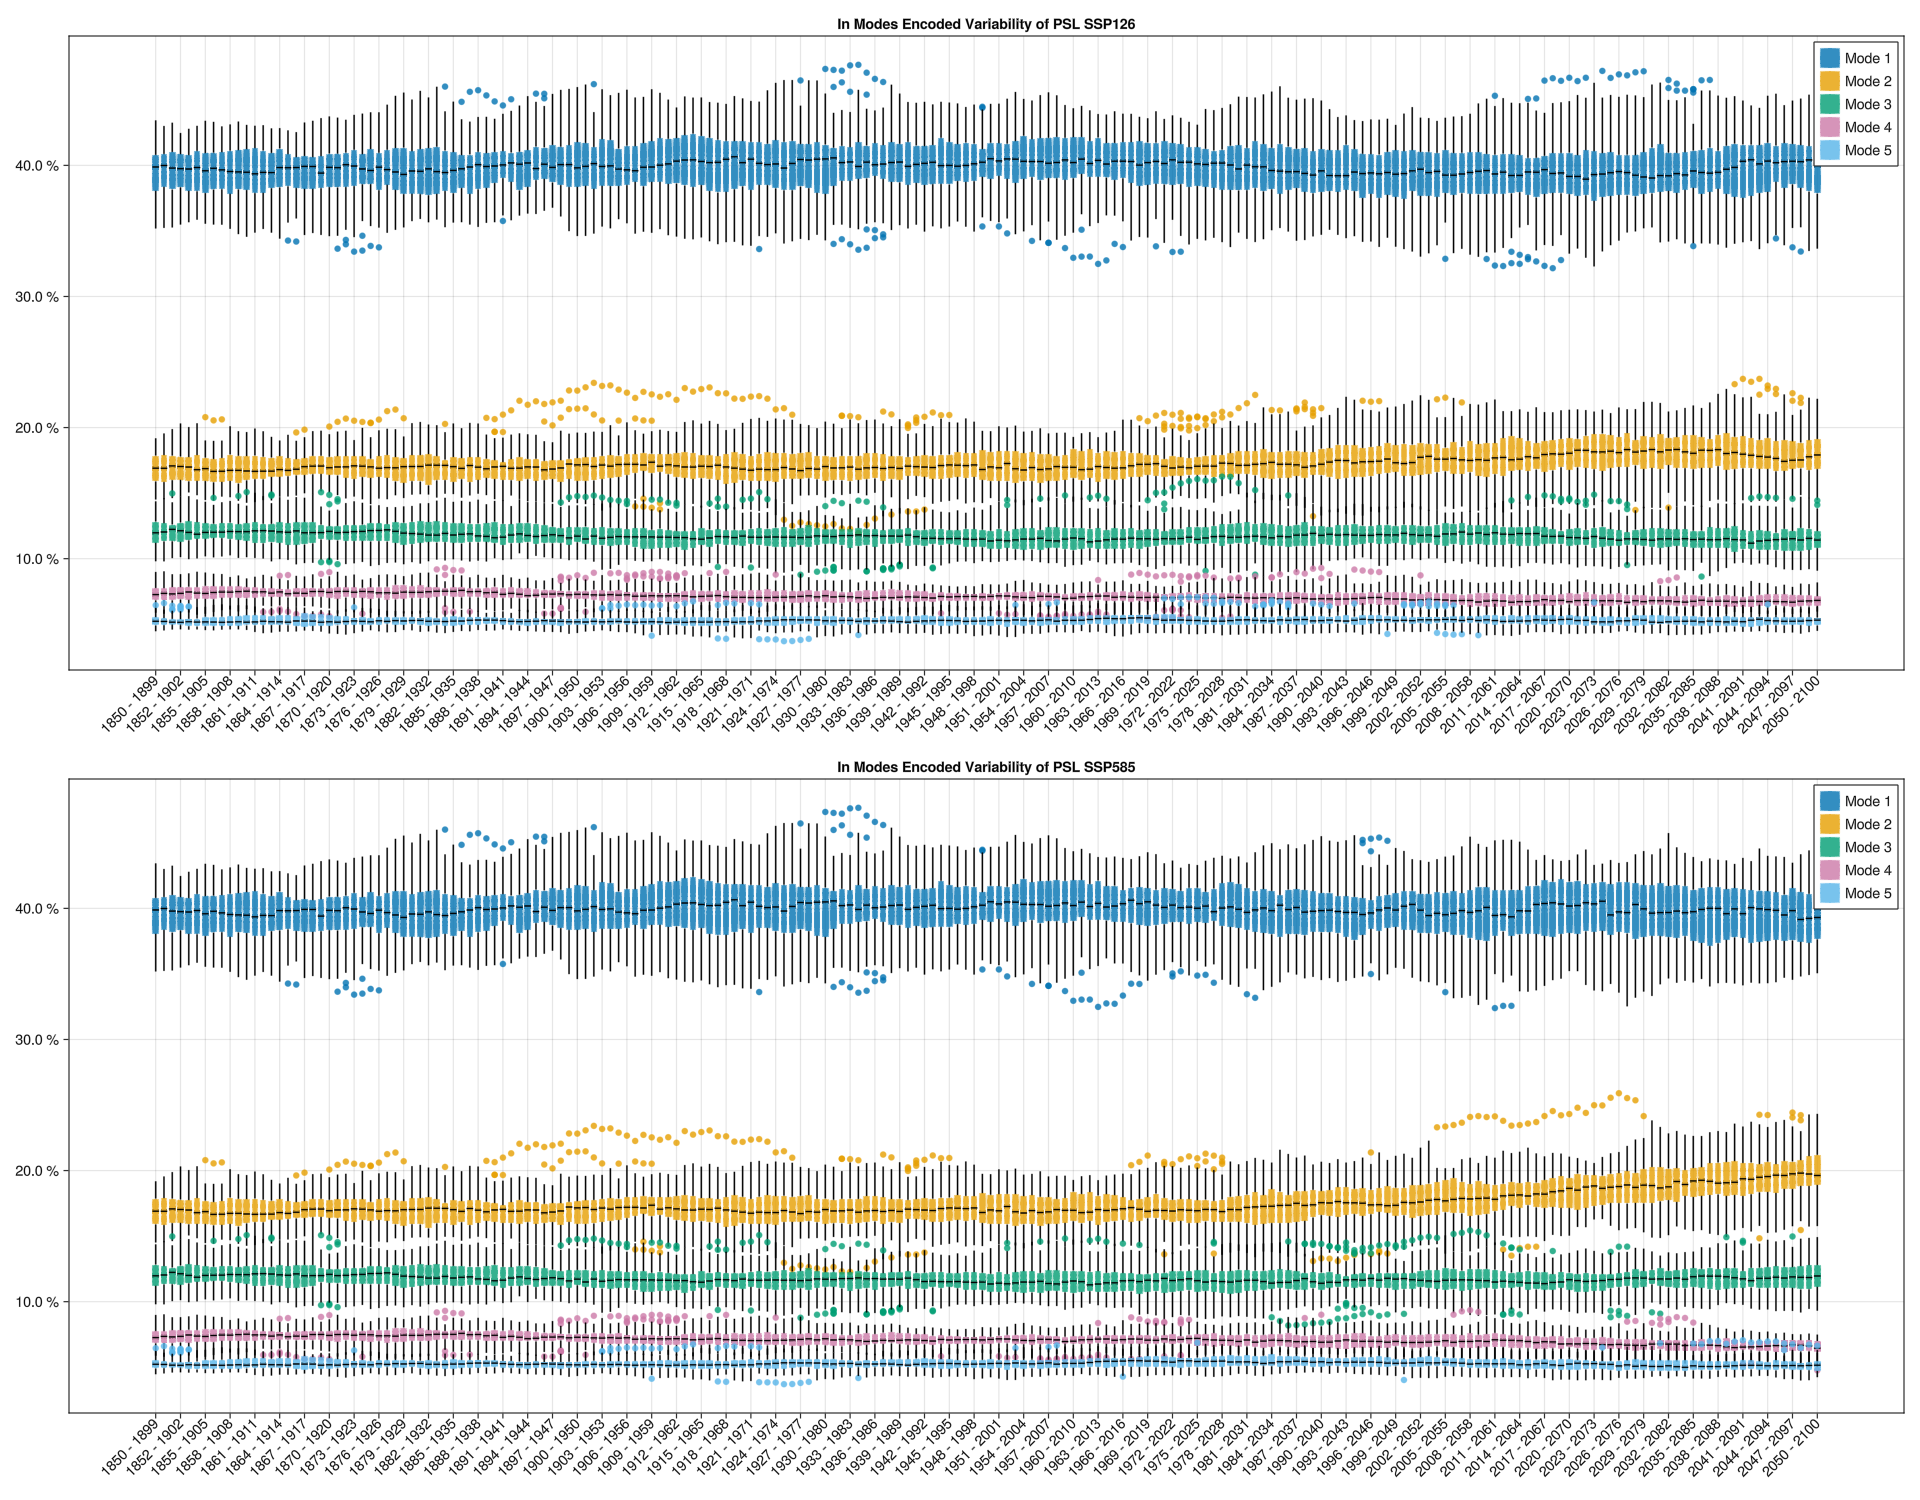
\includegraphics[width=0.85\textwidth]{figures/mode_variability_psl_50seasons.png}
  \end{center}
  \caption{Boxplot of the variability encoded in the top five modes of PSL EOF.}\label{fig:psl mode variability}
\end{figure}

The first simple evaluation is to look at the change of share of variability encoded by each EOF (see Equation~\ref{eq:eof variance calculation}). 
The results are displayed in boxplots, with the colored bar being $50\%$  of the members. 
The whiskers are 1.5 the size of the interquartile range (distance between upper and lower and of the colored bar), any data point outside that is considered an outlier and represented with dots. 


Figure~\ref{fig:psl mode variability} shows that there is no significant change in the SSP126 scenario in any way. 
The five most significant modes stay pretty much the same across the studied 250-year time period, with the primary mode (NAO) encoding around $39\%$ (median) of the whole dataset variability in each time scope, with fluctuations of the interquartile range ($50\%$ of the data) introduced by the members of the simulations being around $\pm 2\%$, with no significant trend over the years. 
The secondary mode (EAP) median stays around $17\%$, with the quartiles being $\pm 1\%$. 
The median variability encoded by EOFs 3,4 and 5 is around $13\%$, $8\%$, and $5\%$, respectively. 
Comparing it to the SSP585 scenario, it is obvious that there is very little to no change in Modes 3-5 and 1. 
But interestingly, the median variability encoded by the secondary mode rises from the $17\%$ in the 1850 - 1900 scope to around $20\%$ in the last one, exposing a clear trend over the course of climate change.   


\begin{figure}[hbt]
  \begin{center}
    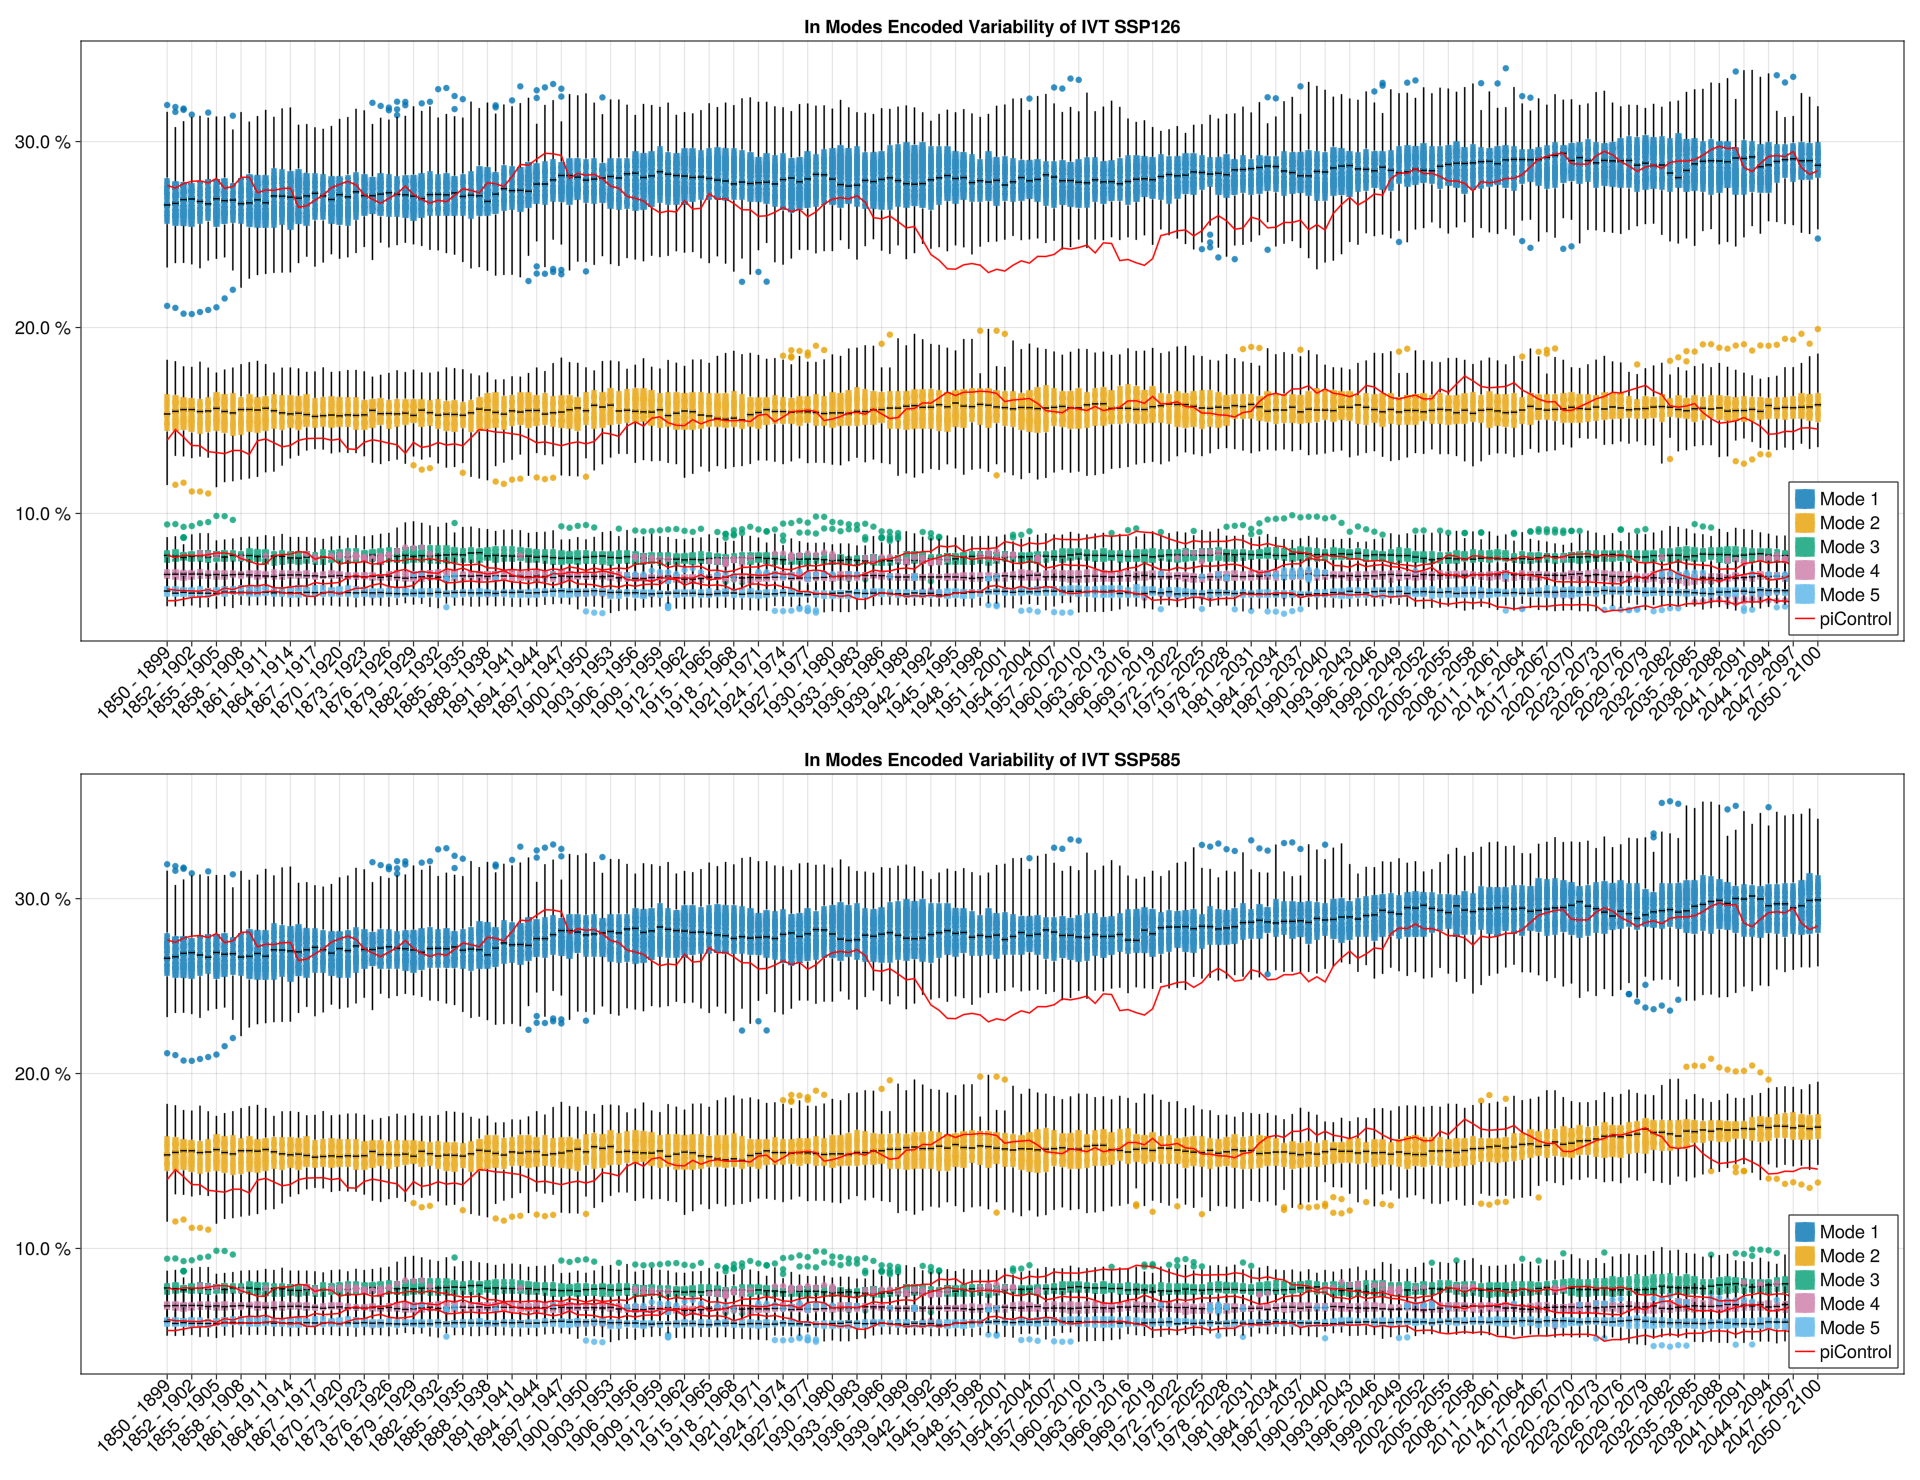
\includegraphics[width=0.85\textwidth]{figures/mode_variability_ivt_50seasons.png}
  \end{center}
  \caption{Same as Figure~\ref{fig:psl mode variability} but with IVT}\label{fig:ivt mode variability}
\end{figure}

The same analysis with the IVT patterns (Figure~\ref{fig:ivt mode variability}) reveal a general upwards trend in the primary mode of IVT, from median $26\%$ in the first window to around $28\%$ in the last. 
This trend is very similar in both SSP126 and SSP 585. 
Modes 3,4 and 5 also look very similar in both evaluated scenarios, with a median encoded variability of $8\%$, $6\%$, and $5\%$. 
Similar to Figure~\ref{fig:psl mode variability}, the secondary mode (representing around $15\%$ of variability) shows upward trend in scenario SSP585 to around $17\%$, which is not recognizable in the SSP126 scenario. 

\begin{figure}[htb]
  \begin{center}
    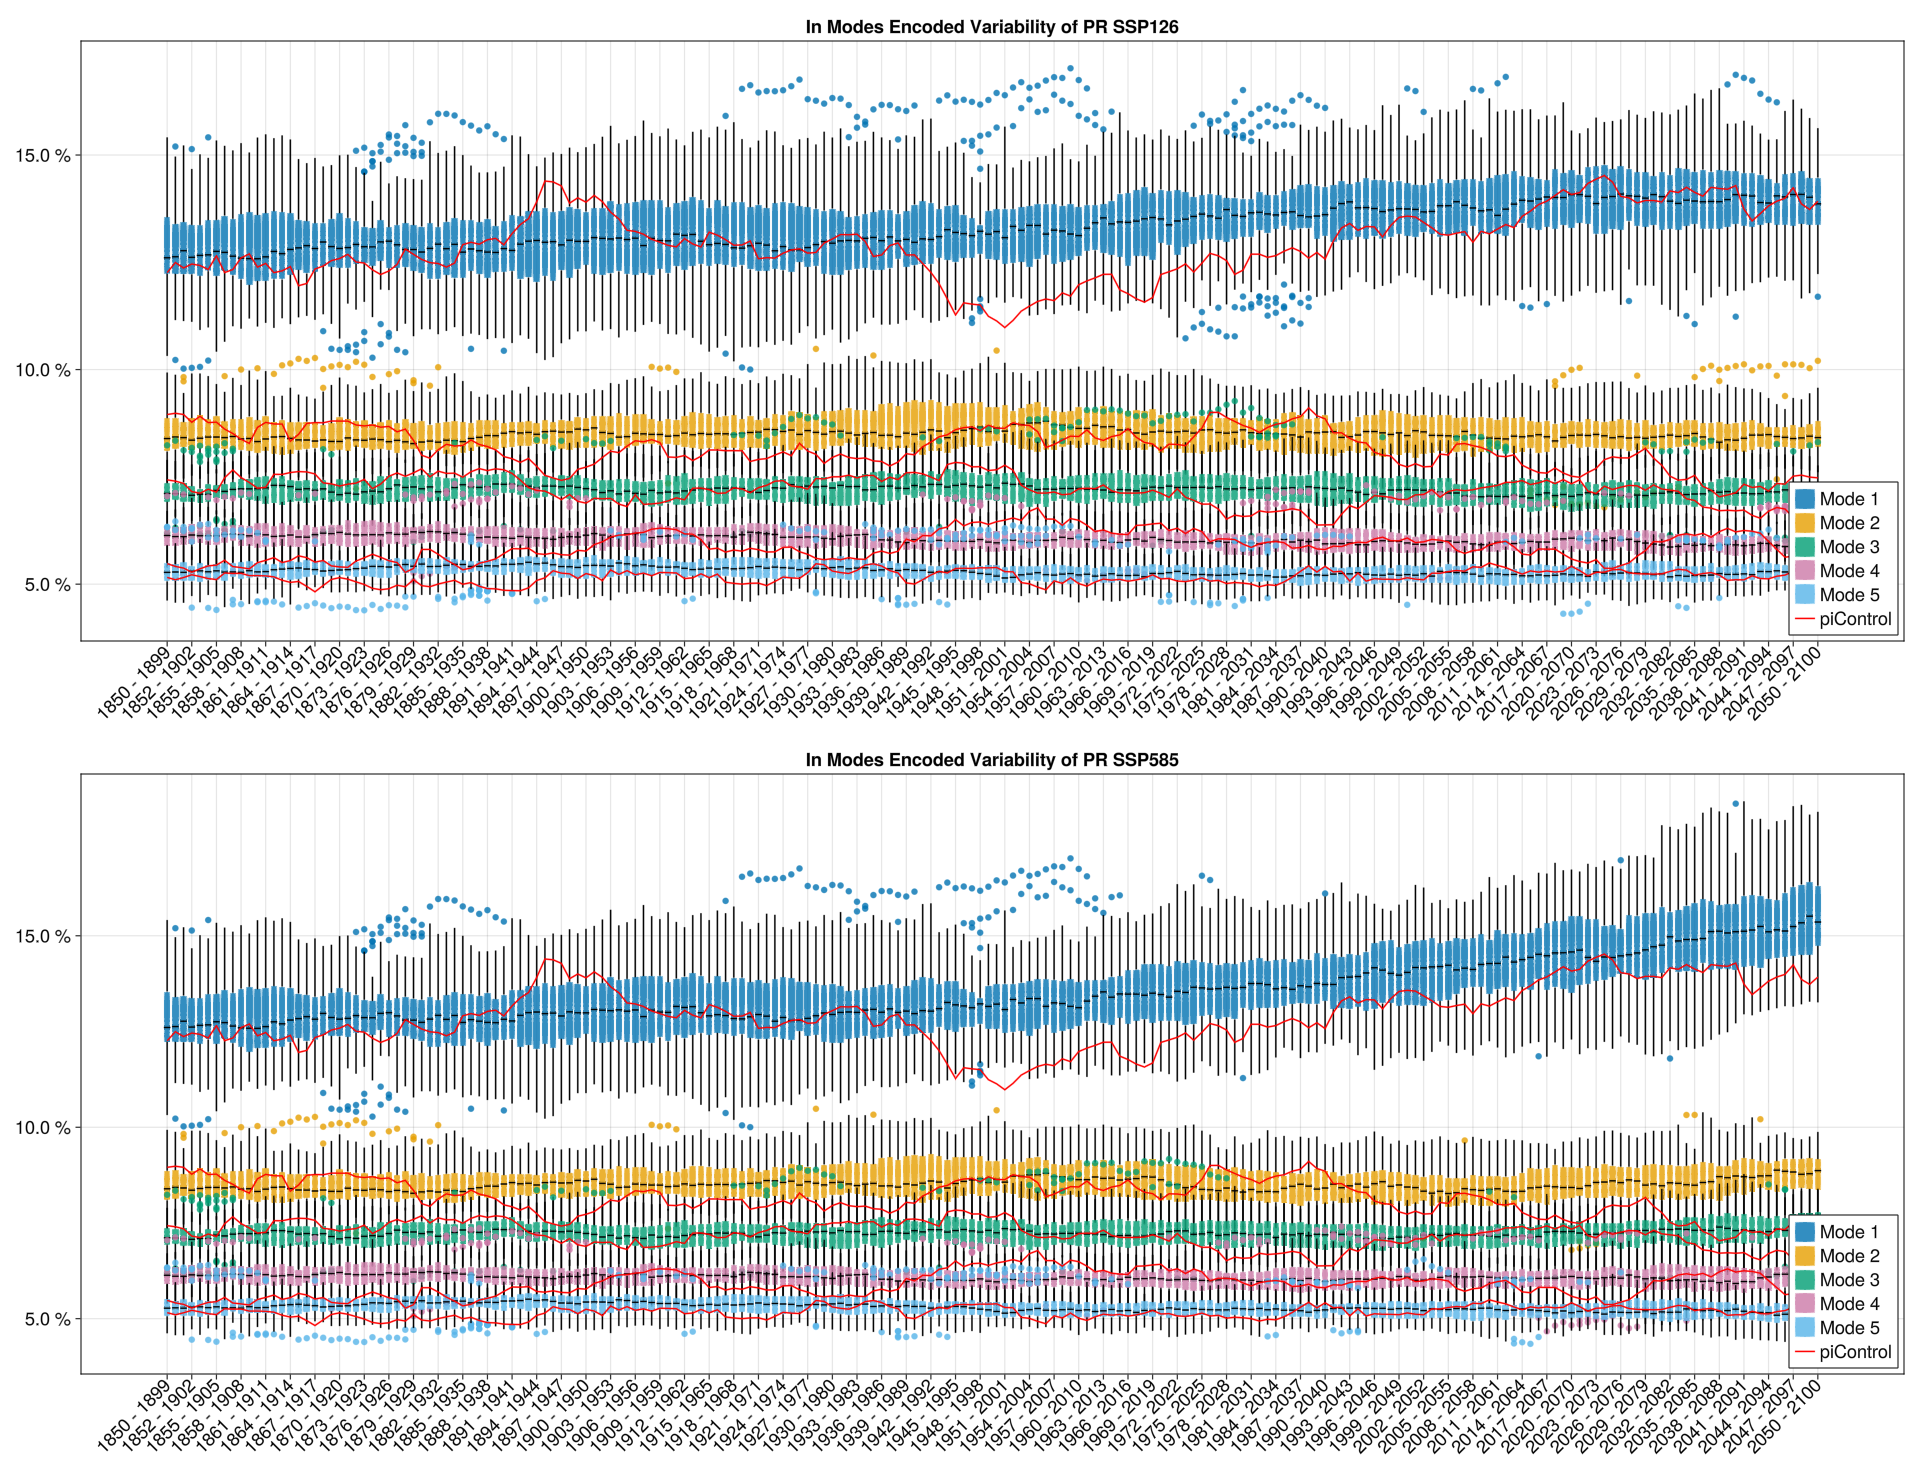
\includegraphics[width=0.85\textwidth]{figures/mode_variability_pr_50seasons.png}
  \end{center}
  \caption{Same as Figure~\ref{fig:psl mode variability} but with precipitation}\label{fig:pr mode variability}
\end{figure}

The dominant modes of precipitation EOF seem to account for far less of the total variance ($28.5 \%$ of the top three modes' mean total variance at the beginning of the historical simulation), compared to the other patterns ($50 \%$ and $68 \%$ for IVT and PSL, respectively).  
The comparison of mode variability evolution of precipitation EOFs (Figure~\ref{fig:pr mode variability}) shows no significant changes of modes 3,4, and 5 between both evaluated scenarios. 
Those encode on median $5\%$, $6\%$ and $6.5\%$ with small fluctuations introduced by the members. 
Mode 2 also looks very similar in both scenarios, with a median encoded variability of around $8.5\%$. 
The primary EOF on the other shows significant differences across scenarios: While it has a far greater variability across members then the other modes and follows a general upwards trend in both SSP126 and SSP585, it is more pronounced in the latter. 
It evolves from around $12.5\%$ in the 1850-1900 window to around $14\%$ in SSP126 and $15.5\%$ in SSP585.  


In general, the modes beyond the second seem to be not well separated from the others, which is why they won't be analyzed in detail in the following sections. 

\subsection{Evolution of Spatial Patterns}
\label{sec:spatial pattern evolution}

\begin{figure}[htb]
  \begin{center}
    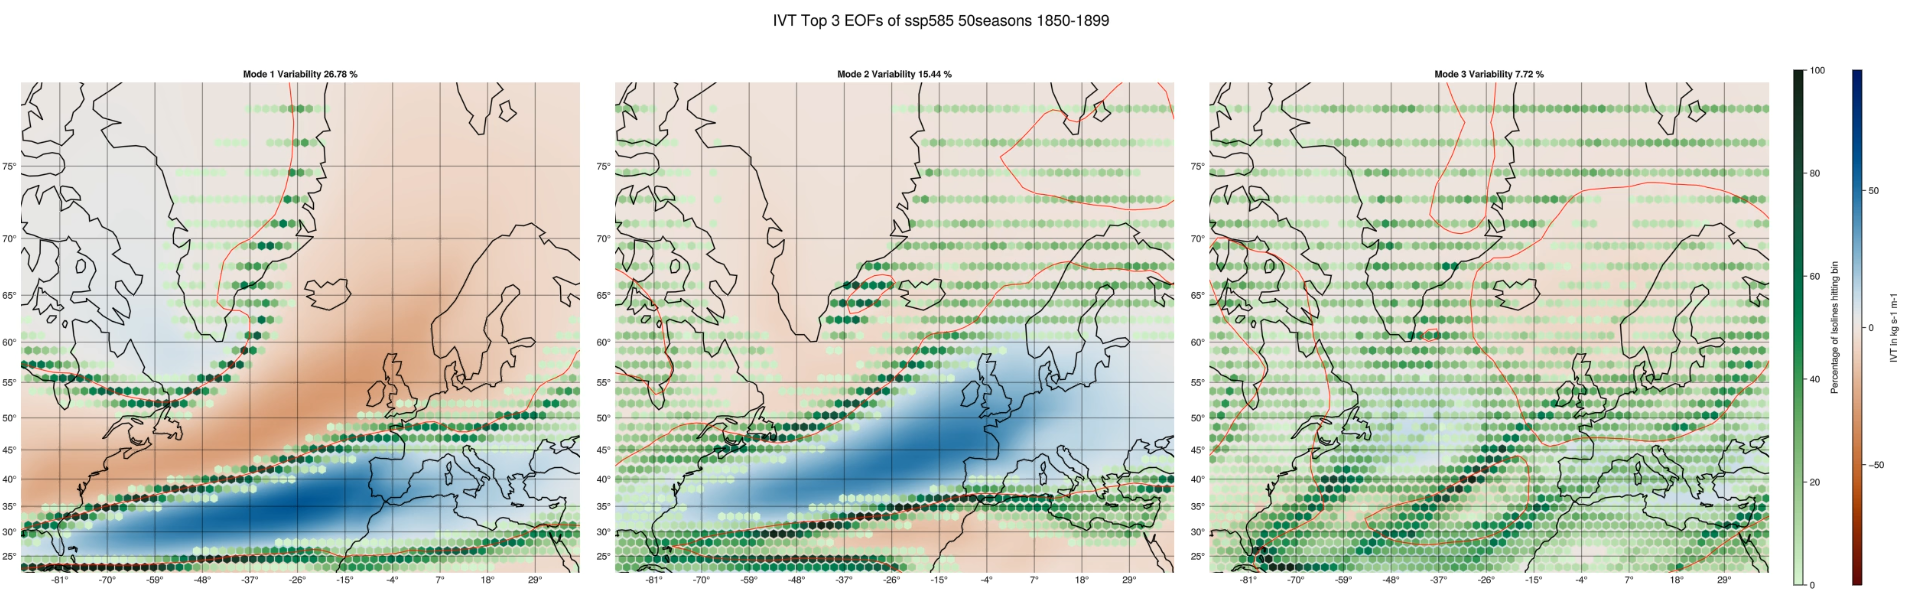
\includegraphics[width=0.85\textwidth]{figures/ivt_spat_patterns_hexbin_18501899_ssp585_50seasons.png}
    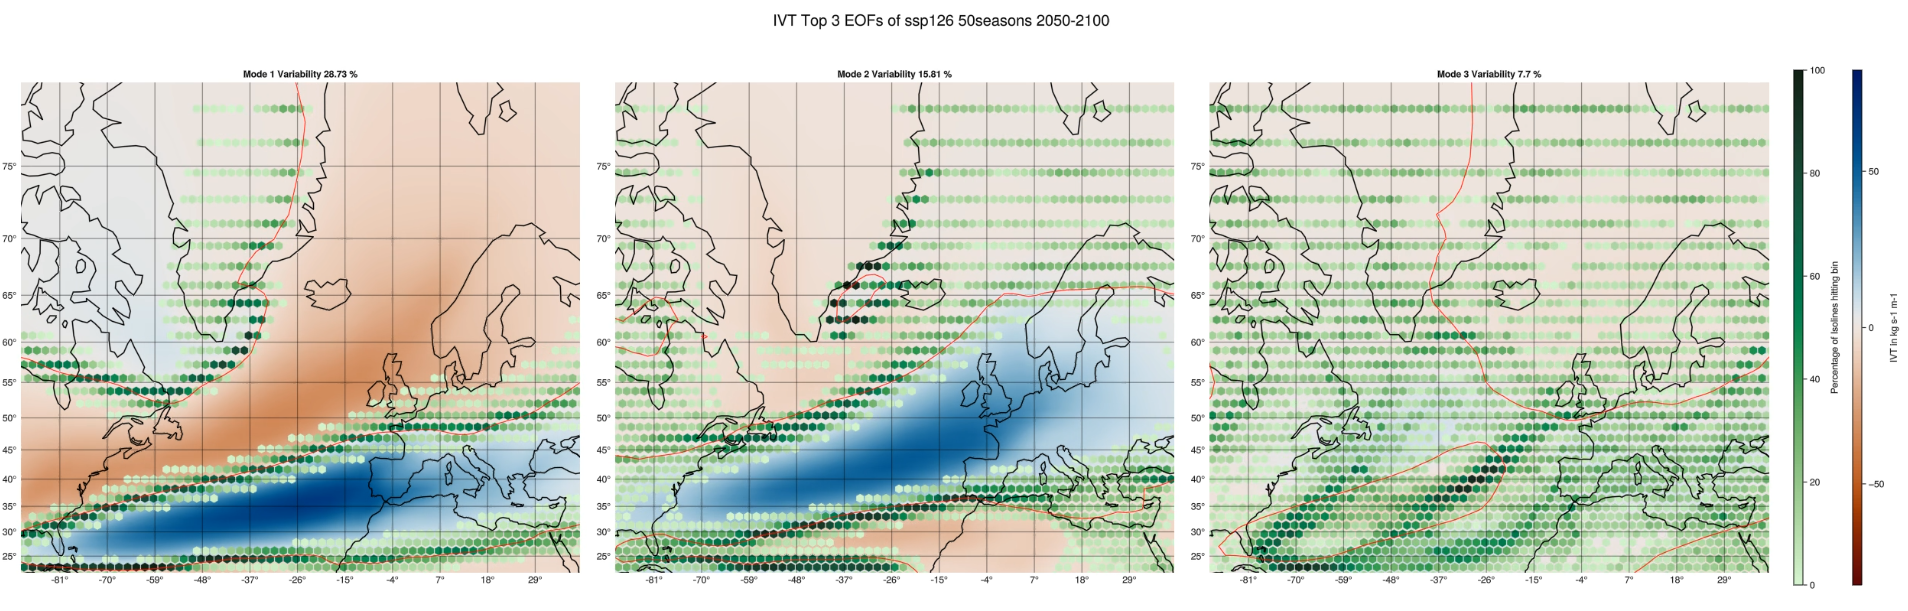
\includegraphics[width=0.85\textwidth]{figures/ivt_spat_patterns_hexbin_20502100_ssp126_50seasons.png}
    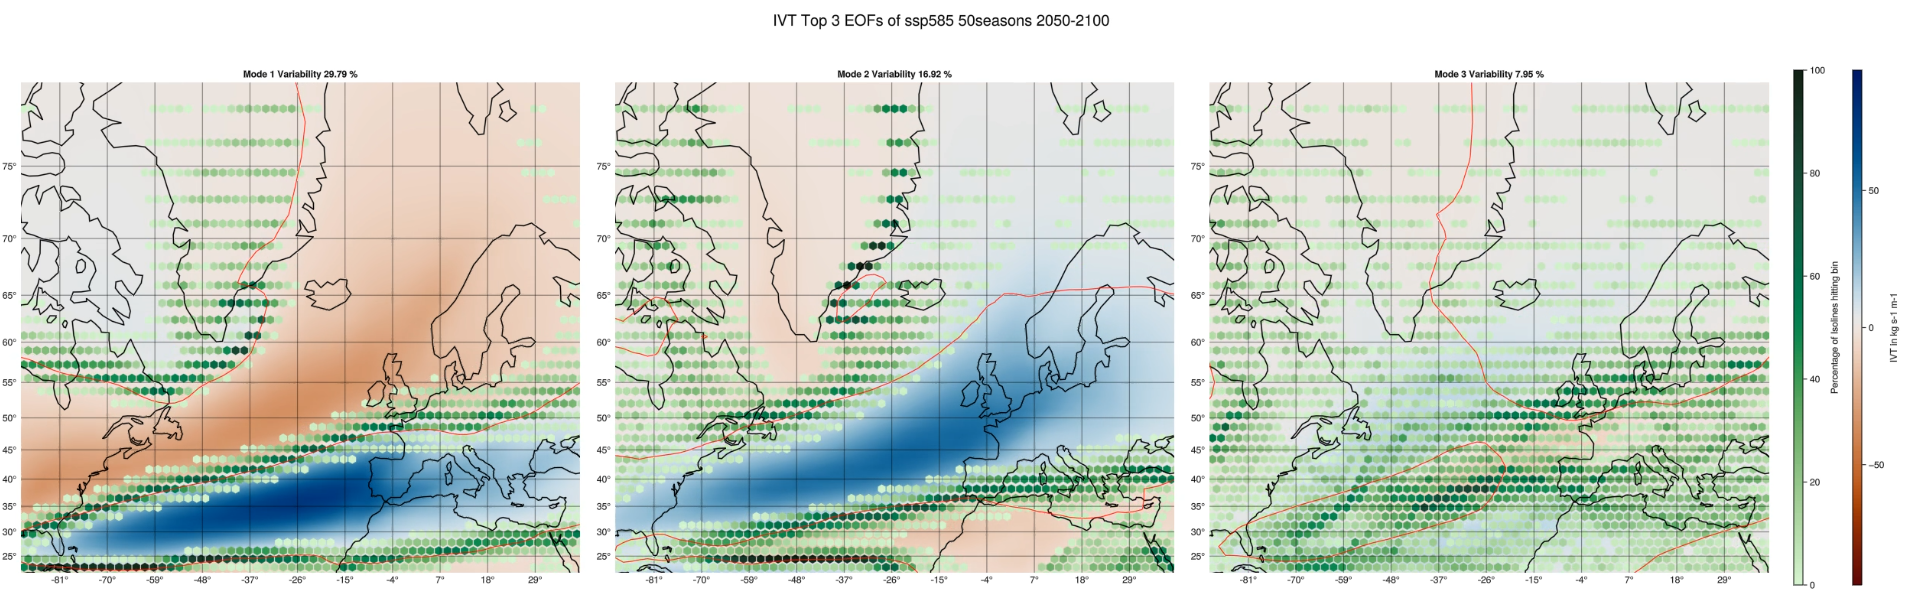
\includegraphics[width=0.85\textwidth]{figures/ivt_spat_patterns_hexbin_20502100_ssp585_50seasons.png}
  \end{center}
  \caption{The top three EOFs of IVT data, with a 50 winter scope and hexbins visualizing the variability introduced by simulation members. The top row displays the state in the historical simulation (second half of 19th century), while middle (SSP126) and bottom (SSP585) display the state in the second half of the 21st century. The red line shows the contour line of zero of the preindustrial control simulation. }\label{fig:ivt eof evolution}
\end{figure}


This Section shows the evolution of the spatial EOF patterns, shown in Figure~\ref{fig:5modes each variable}. 
Since the EOF modes four and five are generally quite low and similar in their eigenvalues (which directly correspond to the variance (see Equation~\ref{eq:eof variance calculation}) encoded shown in Figures~\ref{fig:ivt mode variability}, \ref{fig:psl mode variability}, and \ref{fig:pr mode variability}), they are left out of the analysis of this and the following sections, as modes' eigenvalues need to be well separated from each other \cite{hannachi_empirical_2007}. 
As already mentioned, mode three also seems to be not well separated, but is still shown in the following figures for an example how an inconsistent mode looks (at least for IVT and precipitation), which makes it hard (or even pointless) to evaluate it for an ensemble simulation.  
Usually, the rule of thumb introduced by \citeauthorwork{north_sampling_1982} is used, but since the eigenvalues of the first three modes (or two for precipitation, see Figure~\ref{fig:pr mode variability}), this is left out of this Thesis. 

The variability introduced through the 50 members of the MPI GE CMIP6 is displayed here with the hexbin approach explained in Section~\ref{sec:vis_analysis}, while a discussion of the hexbin visualization compared to the classical spaghetti is given in Section~\ref{sec:discussion}.
The images in this section are the first and last frame from the video displaying the evolution of the different scenarios.\todo{Reference the videos somehow}  

\begin{figure}[htb]
  \begin{center}
    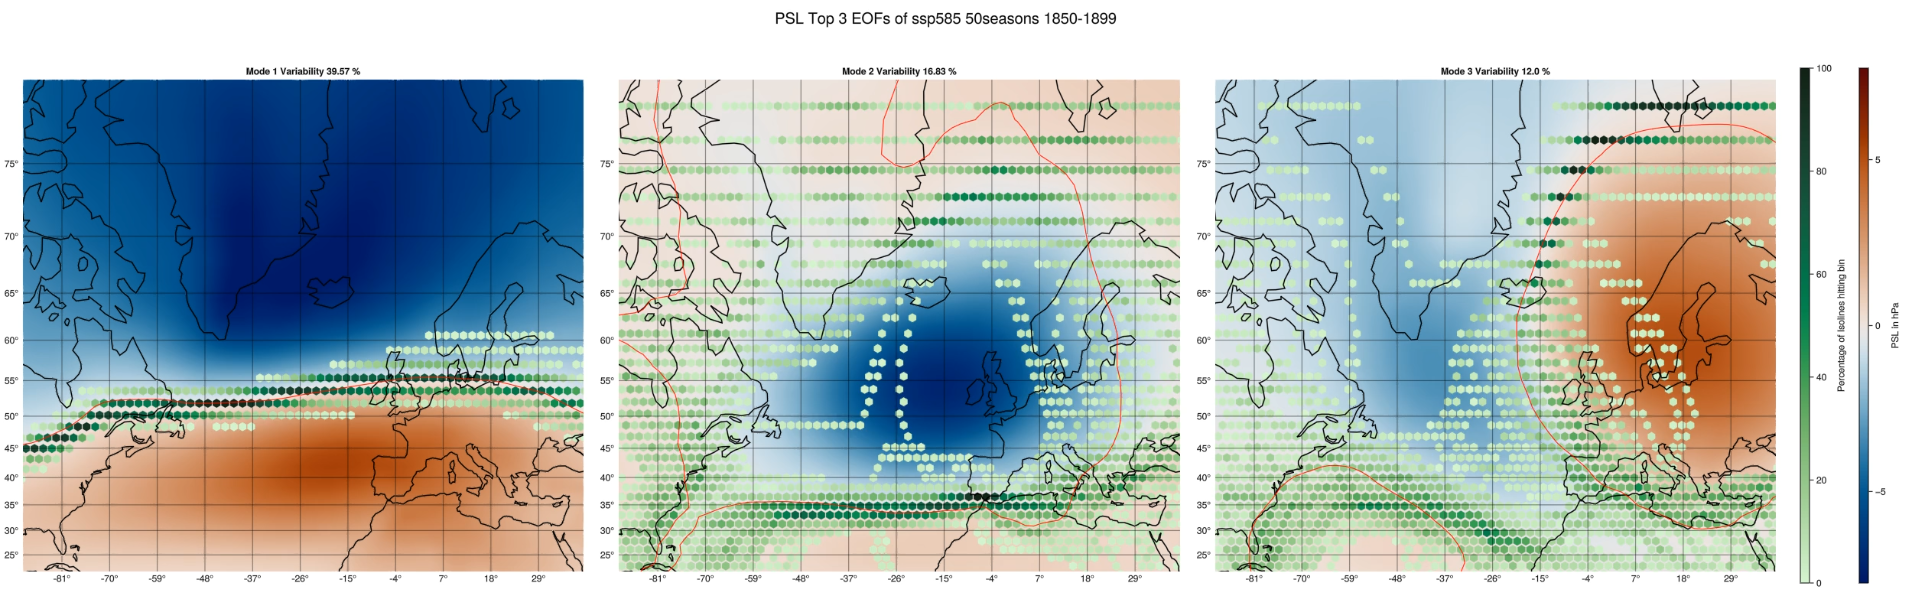
\includegraphics[width=0.85\textwidth]{figures/psl_spat_patterns_hexbin_18501899_ssp585_50seasons.png}
    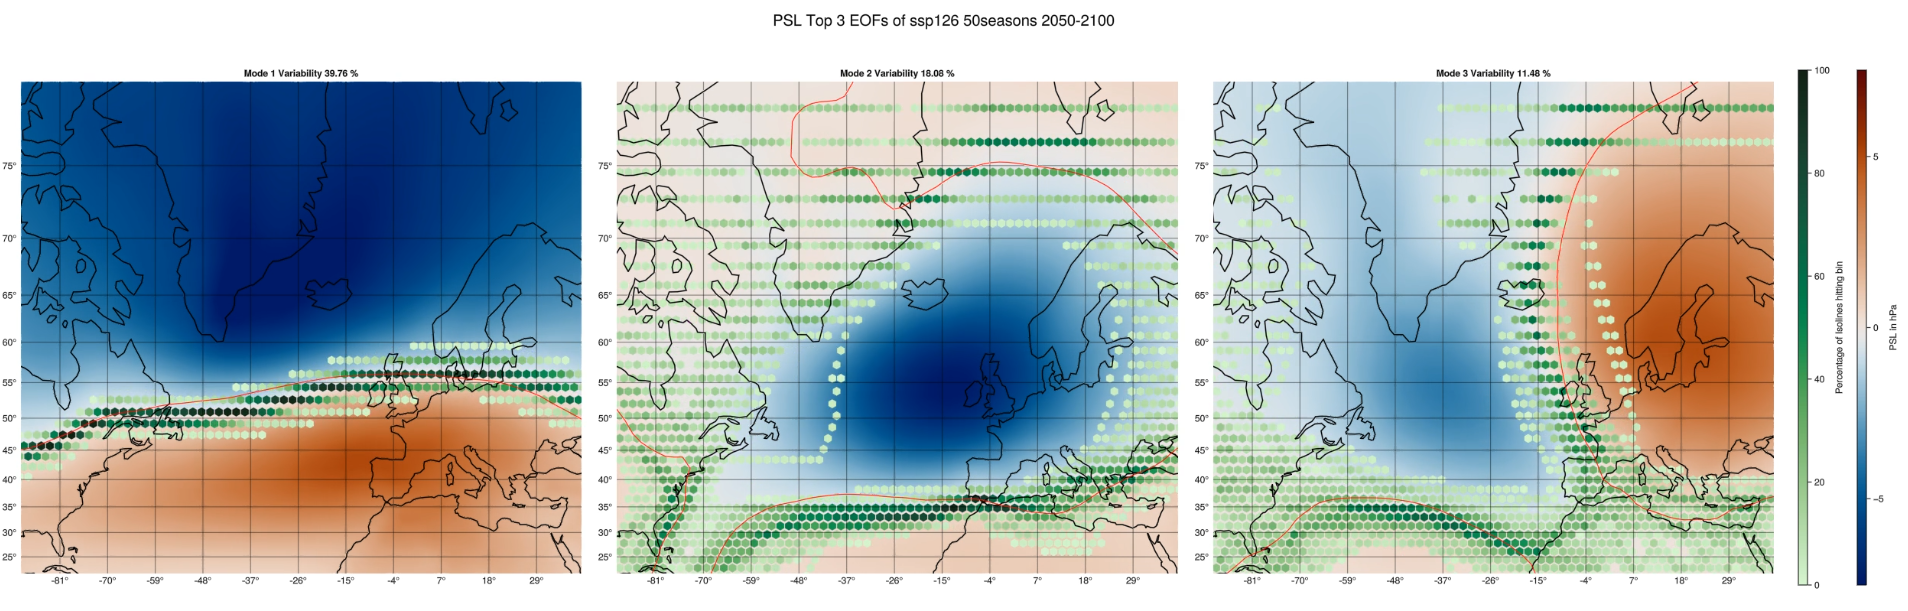
\includegraphics[width=0.85\textwidth]{figures/psl_spat_patterns_hexbin_20502100_ssp126_50seasons.png}
    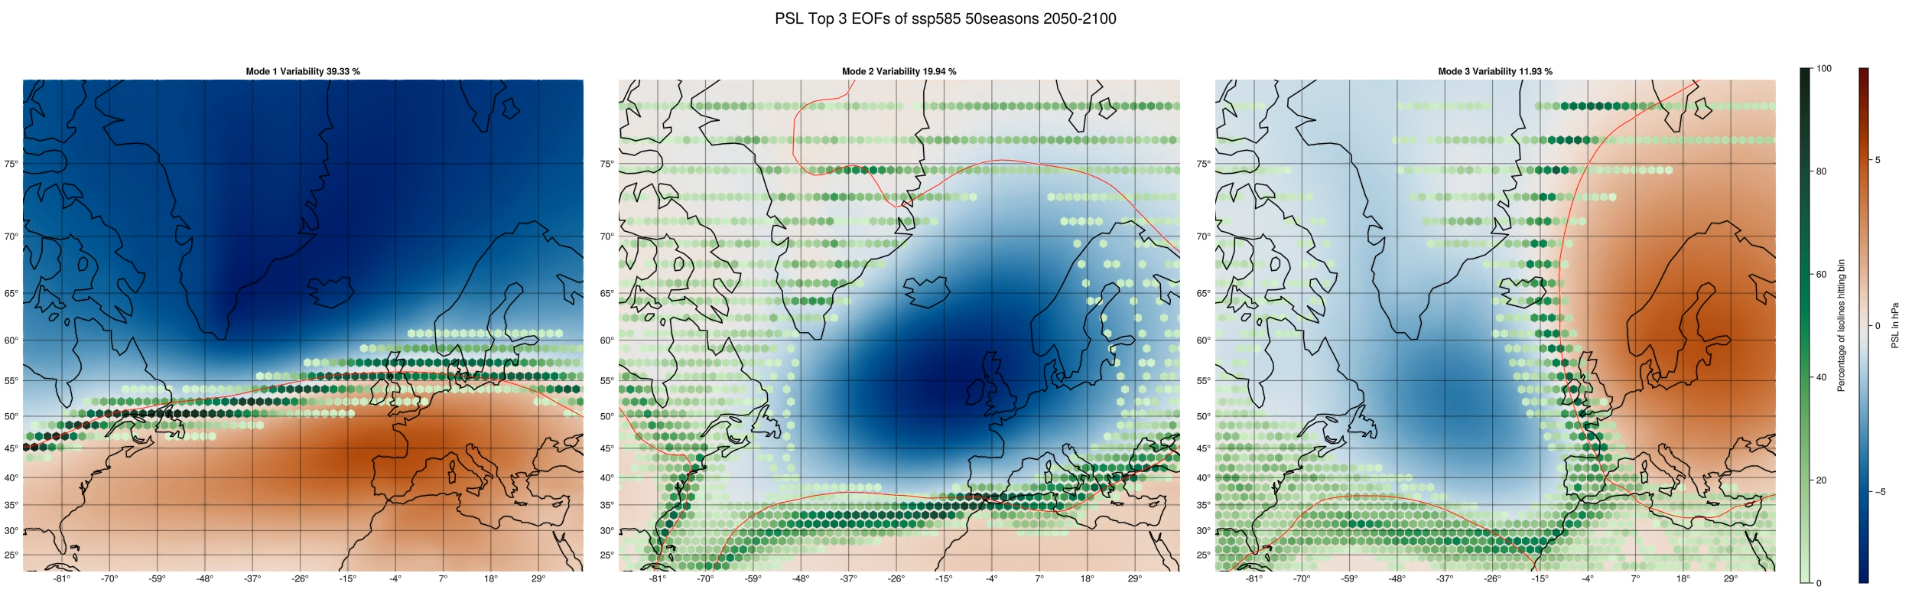
\includegraphics[width=0.85\textwidth]{figures/psl_spat_patterns_hexbin_20502100_ssp585_50seasons.png}
  \end{center}
  \caption{Same as Figure~\ref{fig:ivt eof evolution}, but with sea level pressure data.}\label{fig:psl eof evolution}
\end{figure}




Figure~\ref{fig:ivt eof evolution} shows the evolution of IVT EOF spatial patterns. 
In general, regardless of the future scenario, EOF1 and EOF2 stays structurally very stable across all the ensembles' members, which can be seen on the clear, dark green borders of the colored surfaces. 
EOF3 on the other hand seems pretty unstable, since most of the map is covered in light greed hexagons, which means that the contour lines of zero switch significantly between all the 50 members of the ensemble. 
This also has consequences for the alignment across members and time, which will obviously not work if the patterns differ greatly across time and members. 
Therefor, the analysis regarding such patterns will be kept short since the multi-member, sliding window analysis of such patterns used in this Thesis does not apply very well to such patterns. 

The dominant EOF1 pattern of IVT is characterized by a positive IVT values reaching from Florida to Spain and negative values from the USA east coast to Northern Europe and the Northern Atlantic. 
There are three, clearly visible borders of these positive and negative areas, associated with three groups of contour lines: The first going through Canada, quite coherently across members (many dark green hexagons in a row), and then following the east coast of Greenland, fading out over the mainland quite differently across the members (many light green hexagons in a larger area). 
The second border follows a similar pattern: Starting quite coherent across members at the beginning of the Florida peninsula, over the Atlantic to the east coast of France, and then fading out differently in Eastern Europe. 
The third border goes through the most southern part of the evaluated area, through North Africa and then to the Arabian Peninsula, staying pretty consistent across its path. 
Comparing the state of the patterns at the end of the different future scenario simulations, the change is quite subtle but visible in the area of France and the South of the British Islands:
While the dark green hexagons in the beginning of the historical simulation are on/below the red line of the preindustrial simulation, the majority of zero contour lines in SSP126 seem to be above the preindustrial control contour line. 
In SSP585, the dark green hexagons stretch even further north, indicating that the slight northward shift of IVT EOF1 at the end of the 21st century is even more pronounced. 

The IVT EOF2 is characterized by a strong IVT anomaly right were the seperation contour line of EOF1 is, and lesser, opposite anomalies in the north and south. 
Comparing the beginning of the historical simulation with SSP126, the changes seem only minimal, whereas the difference of SSP585 and the others are far more pronounced: 
While the southern, prominent separation contour line seems to be more variable across members (broader hexbin band), the northern isoline appears to move to the east, opening the pattern up to the north. 
Also, the big area of fading out contour lines in the north of Scandinavia, seems to now be (more or less) uniformly part of the positive anomaly.  
% While the border in Greenland looks very similar at the end of SSP126 and the begin of the historical simulation, 
% On this example a way of interpreting the hexbin visualization is given, which can be applied to the patterns in Figures \ref{fig:pr eof evolution} and \ref{fig:psl eof evolution}. 
While mode three of IVT EOF does expose changes between the different scenarios (again historical simulation and SSP126 look very similar, while SSP585 differs), the patterns seem to be pretty unstable compared to the other, indicated by the whole map being covered in light green hexbins. 
This implies that the contour lines of zero are all over the map, which means that the structures are quite different across the simulations' members. 

\begin{figure}[htb]
  \begin{center}
    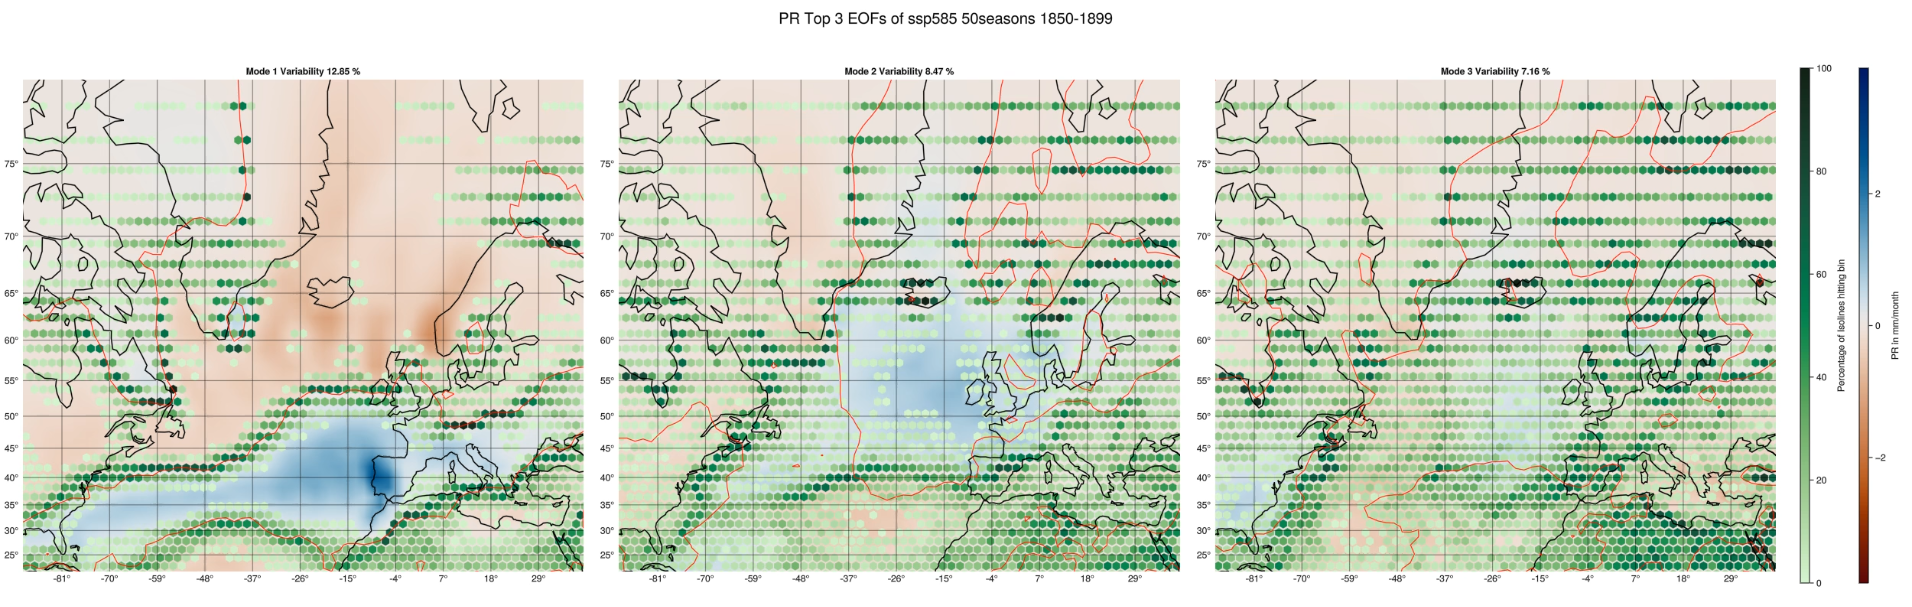
\includegraphics[width=0.85\textwidth]{figures/pr_spat_patterns_hexbin_18501899_ssp585_50seasons.png}
    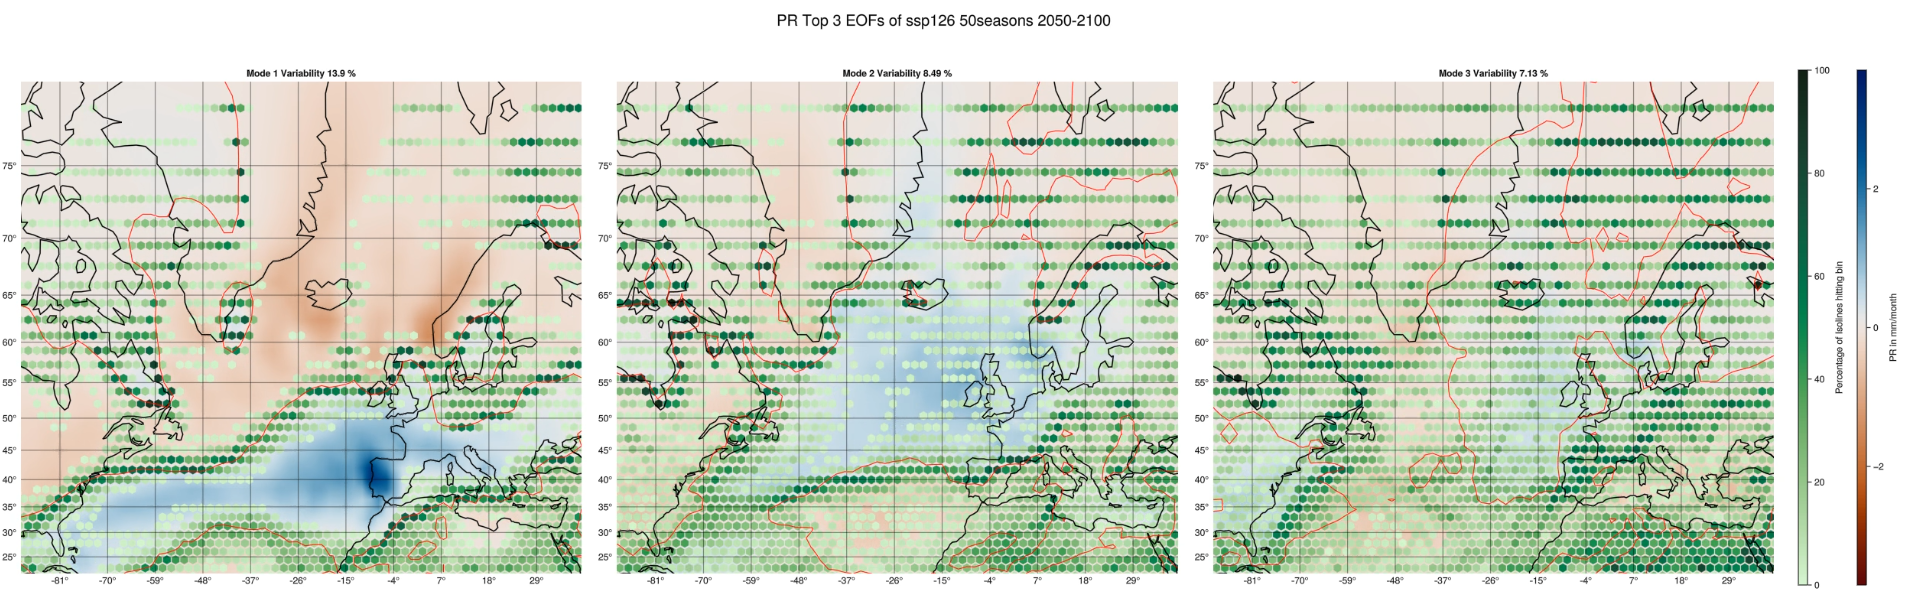
\includegraphics[width=0.85\textwidth]{figures/pr_spat_patterns_hexbin_20502100_ssp126_50seasons.png}
    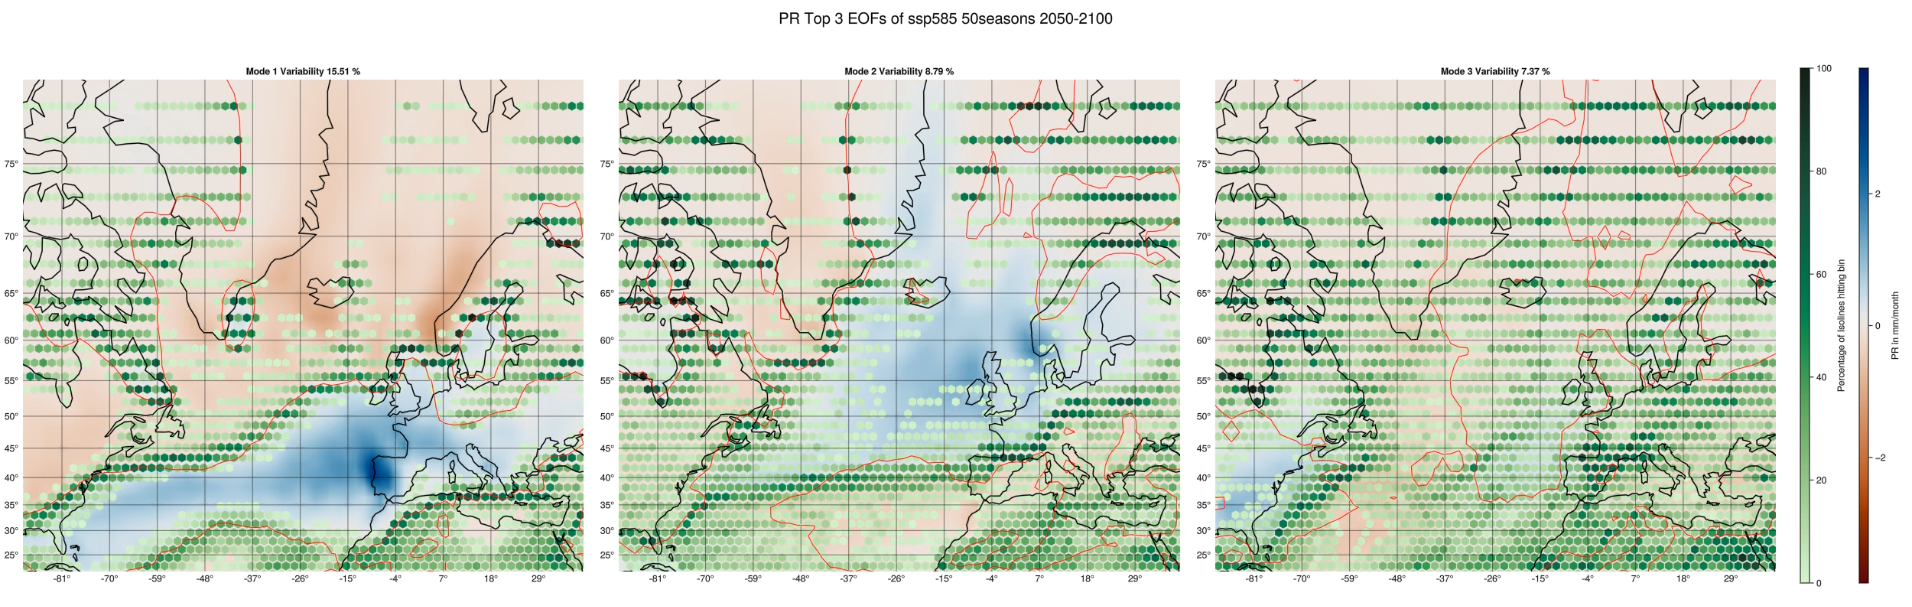
\includegraphics[width=0.85\textwidth]{figures/pr_spat_patterns_hexbin_20502100_ssp585_50seasons.png}
  \end{center}
  \caption{Same as Figure~\ref{fig:ivt eof evolution}, but with precipitation data.}\label{fig:pr eof evolution}
\end{figure}



The evolution of sea level pressure patterns is displayed in Figure~\ref{fig:psl eof evolution}, showing the North Atlantic Oscillation  and the East Atlantic Pattern (see Section~\ref{sec:nao}). 
While the first two EOFs are well known, real world phenomena, the third mode was never mentioned in the related literature. 
Although it seems to be stable across members and time scopes, it will therefor be left out of the analysis. 
The NAO in mode one, characterized by its north-south dipole of pressure, is very consistent across the 50 members of the simulation, indicated by the narrow band of hexbins showing the switching line between the positive/negative anomalies. 
Comparing the historical simulation with SSP585, there seems to be a slight northward shift of the hexbin band, best visible at the northern part of the British Islands. 
This shift seems to be less pronounced in SSP126. 
The NAO exhibits no outliers across all the sliding windows. In contrast, the EAP appears deformed in some members, as evidenced by a few very lightly colored hexbins in the blue center of the historical part. These deformations are also observable in other scopes throughout the simulations, unrelated to the historical part of the timeline.
The southern border of the prominent negative pattern remains indistinguishable between the scenarios and the historical simulation. However, the stable northern border, marked by dark green hexbins, seems to shift further north, particularly in SSP585.


Similar to the other Figures in this Section, Figure~\ref{fig:pr eof evolution} shows the evolution of dominant precipitation EOF patterns. 
While mode one looks very similar to the primary pattern of IVT EOF, the secondary mode looks quite comparable to the EAP. 
Quite noticeable in the primary pattern is the strong positive precipitation anomaly at the west coast of the Iberian Peninsula. 
Also, EOF1 is associated with negative anomalies along the southern east coast of Norway and a small positive pattern at the south-western coast of Greenland. 
The SSP126 EOF1 pattern extends considerably into mainland Europe and also extends further north. 
This effect is noticeable only in Europe and not in the Atlantic, with the anomaly along the coast of the Iberian Peninsula becoming more pronounced (indicated by a more intense blue). 
In the SSP585 EOF1 pattern, the effects observed in SSP126 are even more pronounced, with the piControl line comparable to the farthest outliers of SSP585.
% - negative anomalies at the southern east coast of norway
% - SSP126 EOF1 pattern: extends into mainland europe quite a bit, also entends to the north. Effect only noticeable in Europe, not the Atlantic. Also the Anomaly on the coast of Iberian Peninsula got larger (more intense blue)
% - SSP585 EOF1 pattern: effects of SSP126 are more pronounced, piControl line is compareable to outliers of SSP585 
EOF2 of precipitation appears to be quite unstable across the members of the simulations, as indicated by hexbins filling most of the map. The only somewhat stable area is a positive anomaly over Great Britain and slightly further north. A small but consistent negative anomaly is observed along the east coast of Iceland in many members. However, this stability collapses in some members and time steps, as shown by very light green hexbins moving through the center. In future scenarios, the central positive pattern opens up to the north, resembling the evolution of the EAP. This effect is more pronounced in SSP585 than in SSP126.

% - EOF2 of precipitation seems also not very stable across the simulations' members (indicated by hexbins filling most of the map)
% - only area somewhat stable: positive anomaly over great britain and a bit more north. 
% - small but consistent in many members: small negative anomaly at the east coast of iceland 
% - but this also collapses in some members and timesteps, indicated by very light green hexbins moving through the center 
% - Effect in future scenarios: Central positive pattern opens up to the north, similar to the evolution of the EAP 
% - this is more pronounced in SSP585 then in SSP126


\subsection{Evolution of Temporal Patterns}

\begin{figure}[htb]
  \begin{center}
    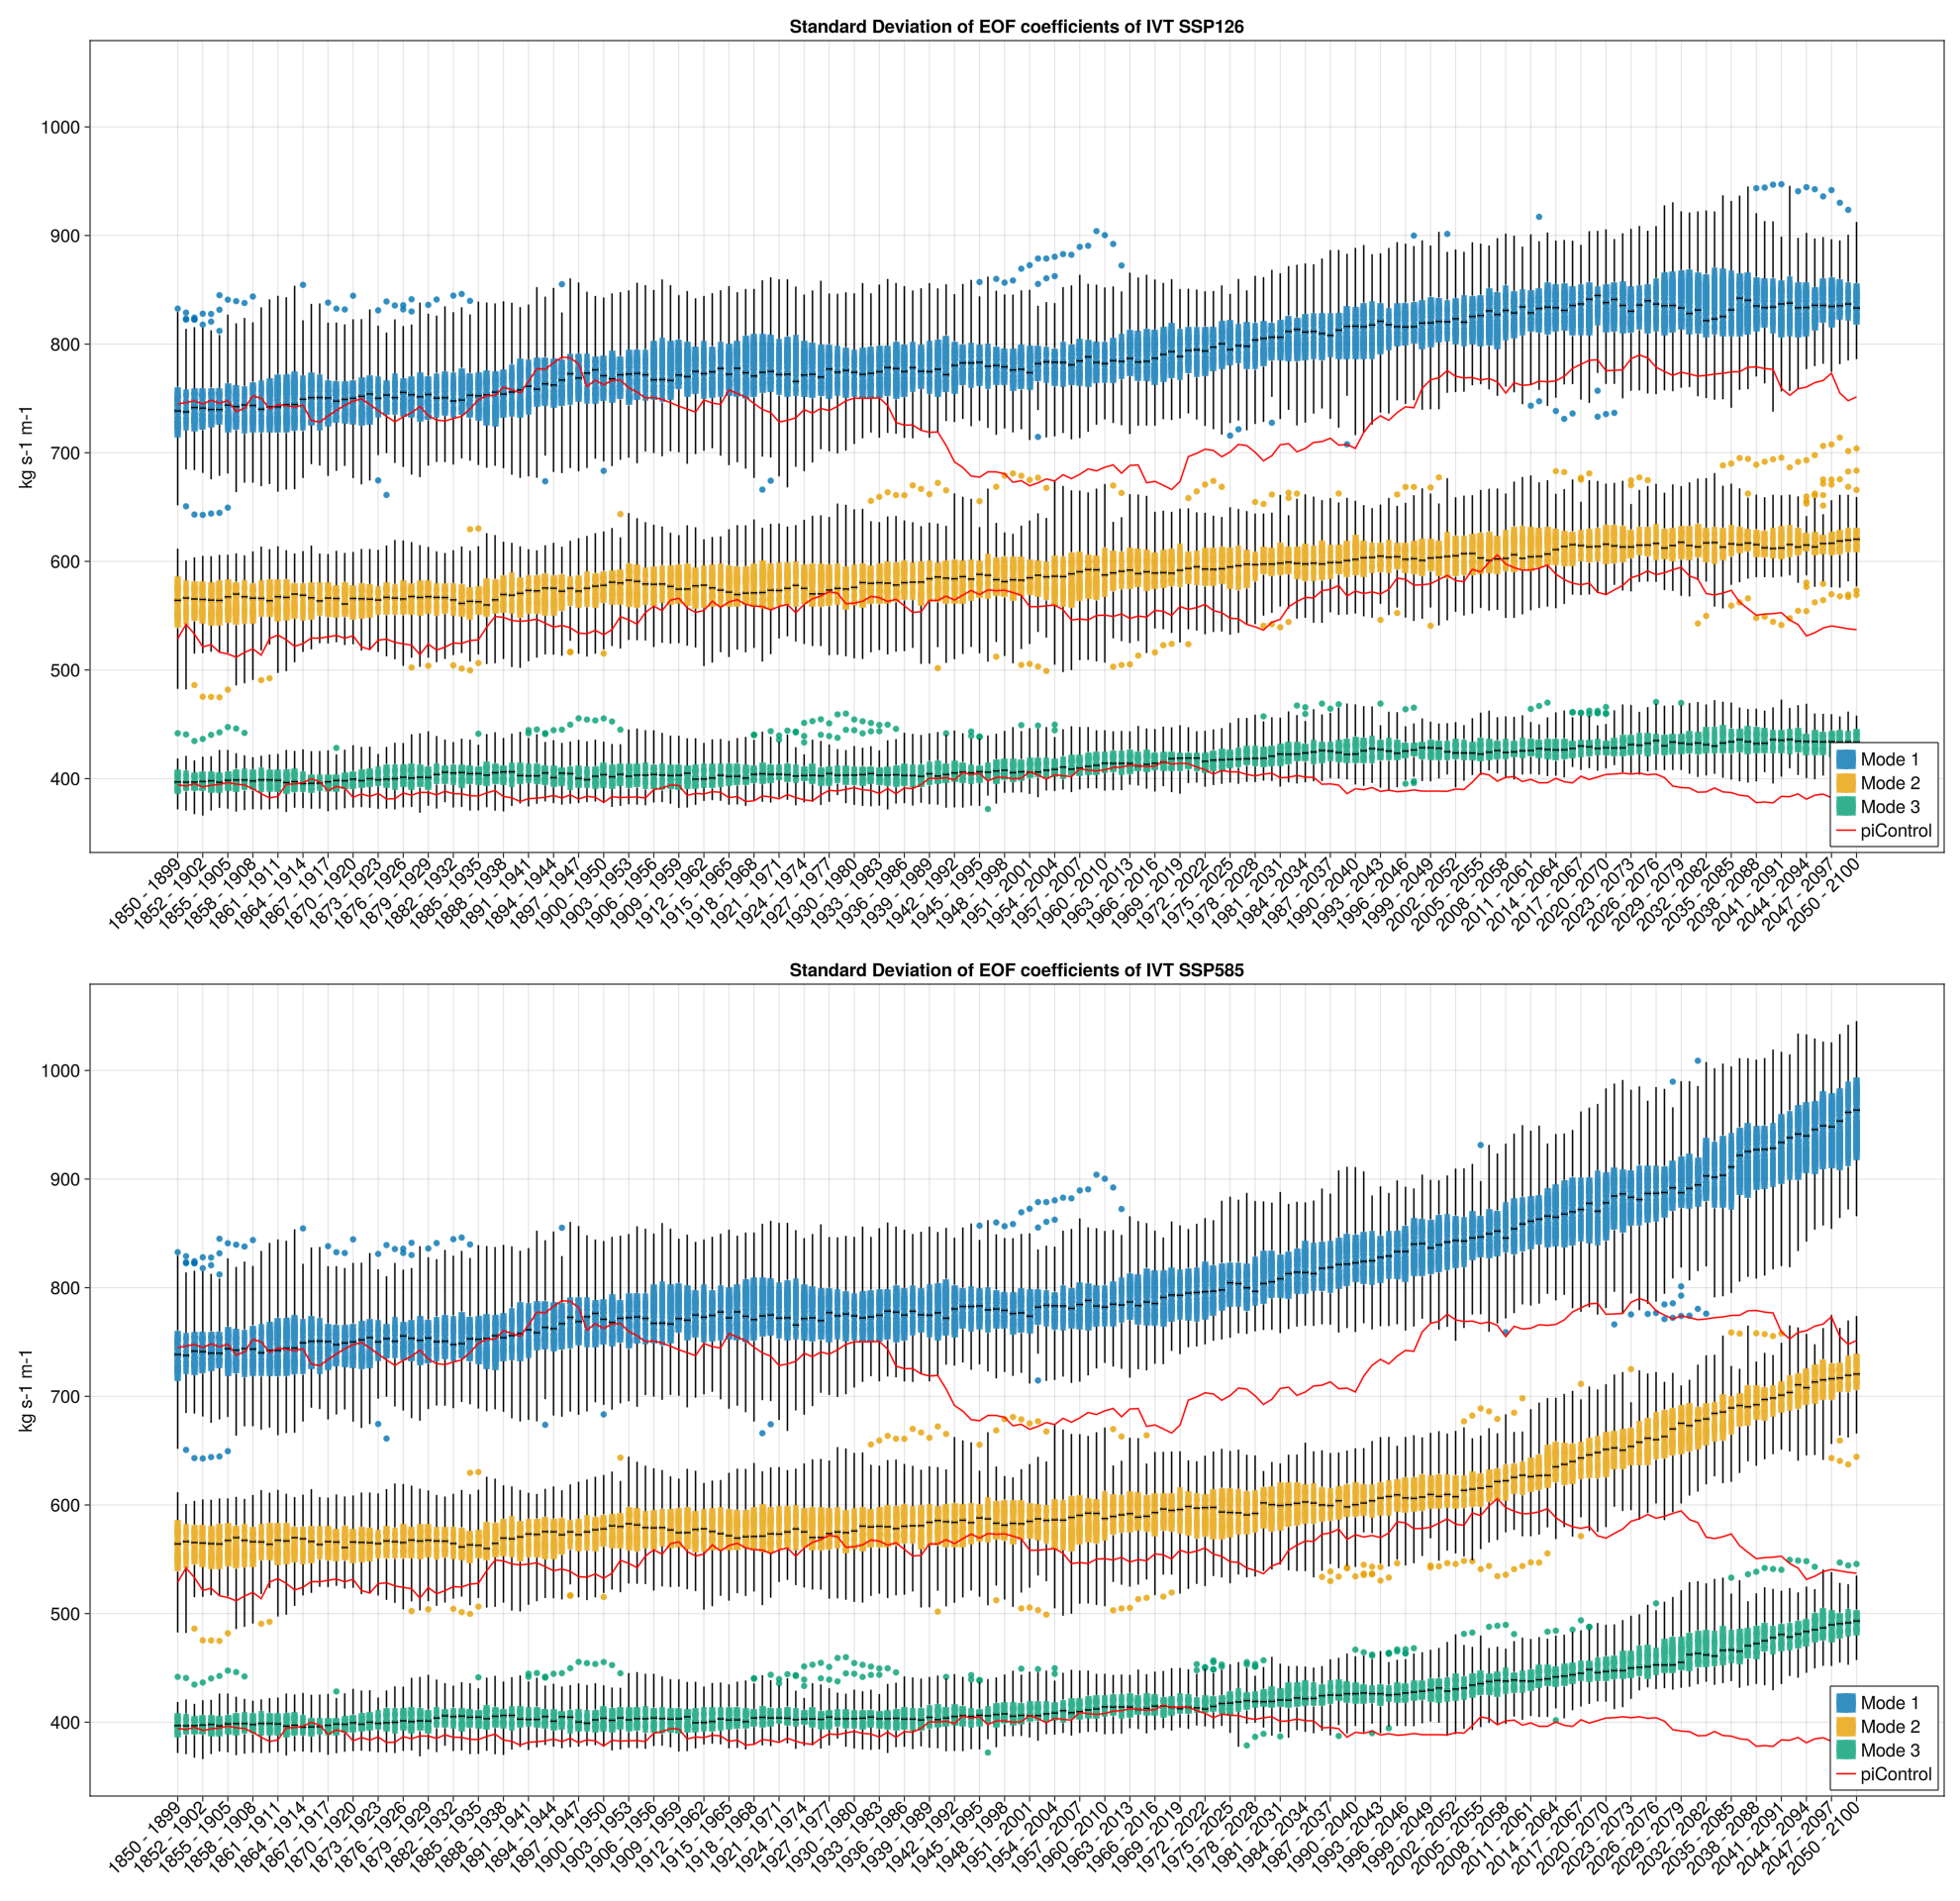
\includegraphics[width=0.65\textwidth]{figures/std_ivt_50seasons_tempmodescale_3modes.png}
  \end{center}
  \caption{Evolution of the standard deviation of IVT EOF coefficients for each scope and simulation member.}
  \label{fig:std ivt evolution}
\end{figure}

As already explained in Section~\ref{sec:vis_analysis}, there is no proper way to visualize the EOF coefficients of an ensemble in the same way related work did it. 
Therefor, the only way left is to analyze statistics of those signals and compare them in a boxplot to get a sense of variability across members. 
In the Figures~\ref{fig:std ivt evolution}, \ref{fig:std psl evolution}, and \ref{fig:std pr evolution} the evolution of the standard deviation (SD) of IVT, sea level pressure, and precipitation is displayed, respectively. 
Keep in mind that being scaled to the original unit means multiplying each EOF coefficient series with the associated singular value, which is very closely related to the encoded variance (see Equation~\ref{eq:eof variance calculation}). 


\begin{figure}[htb]
  \begin{center}
    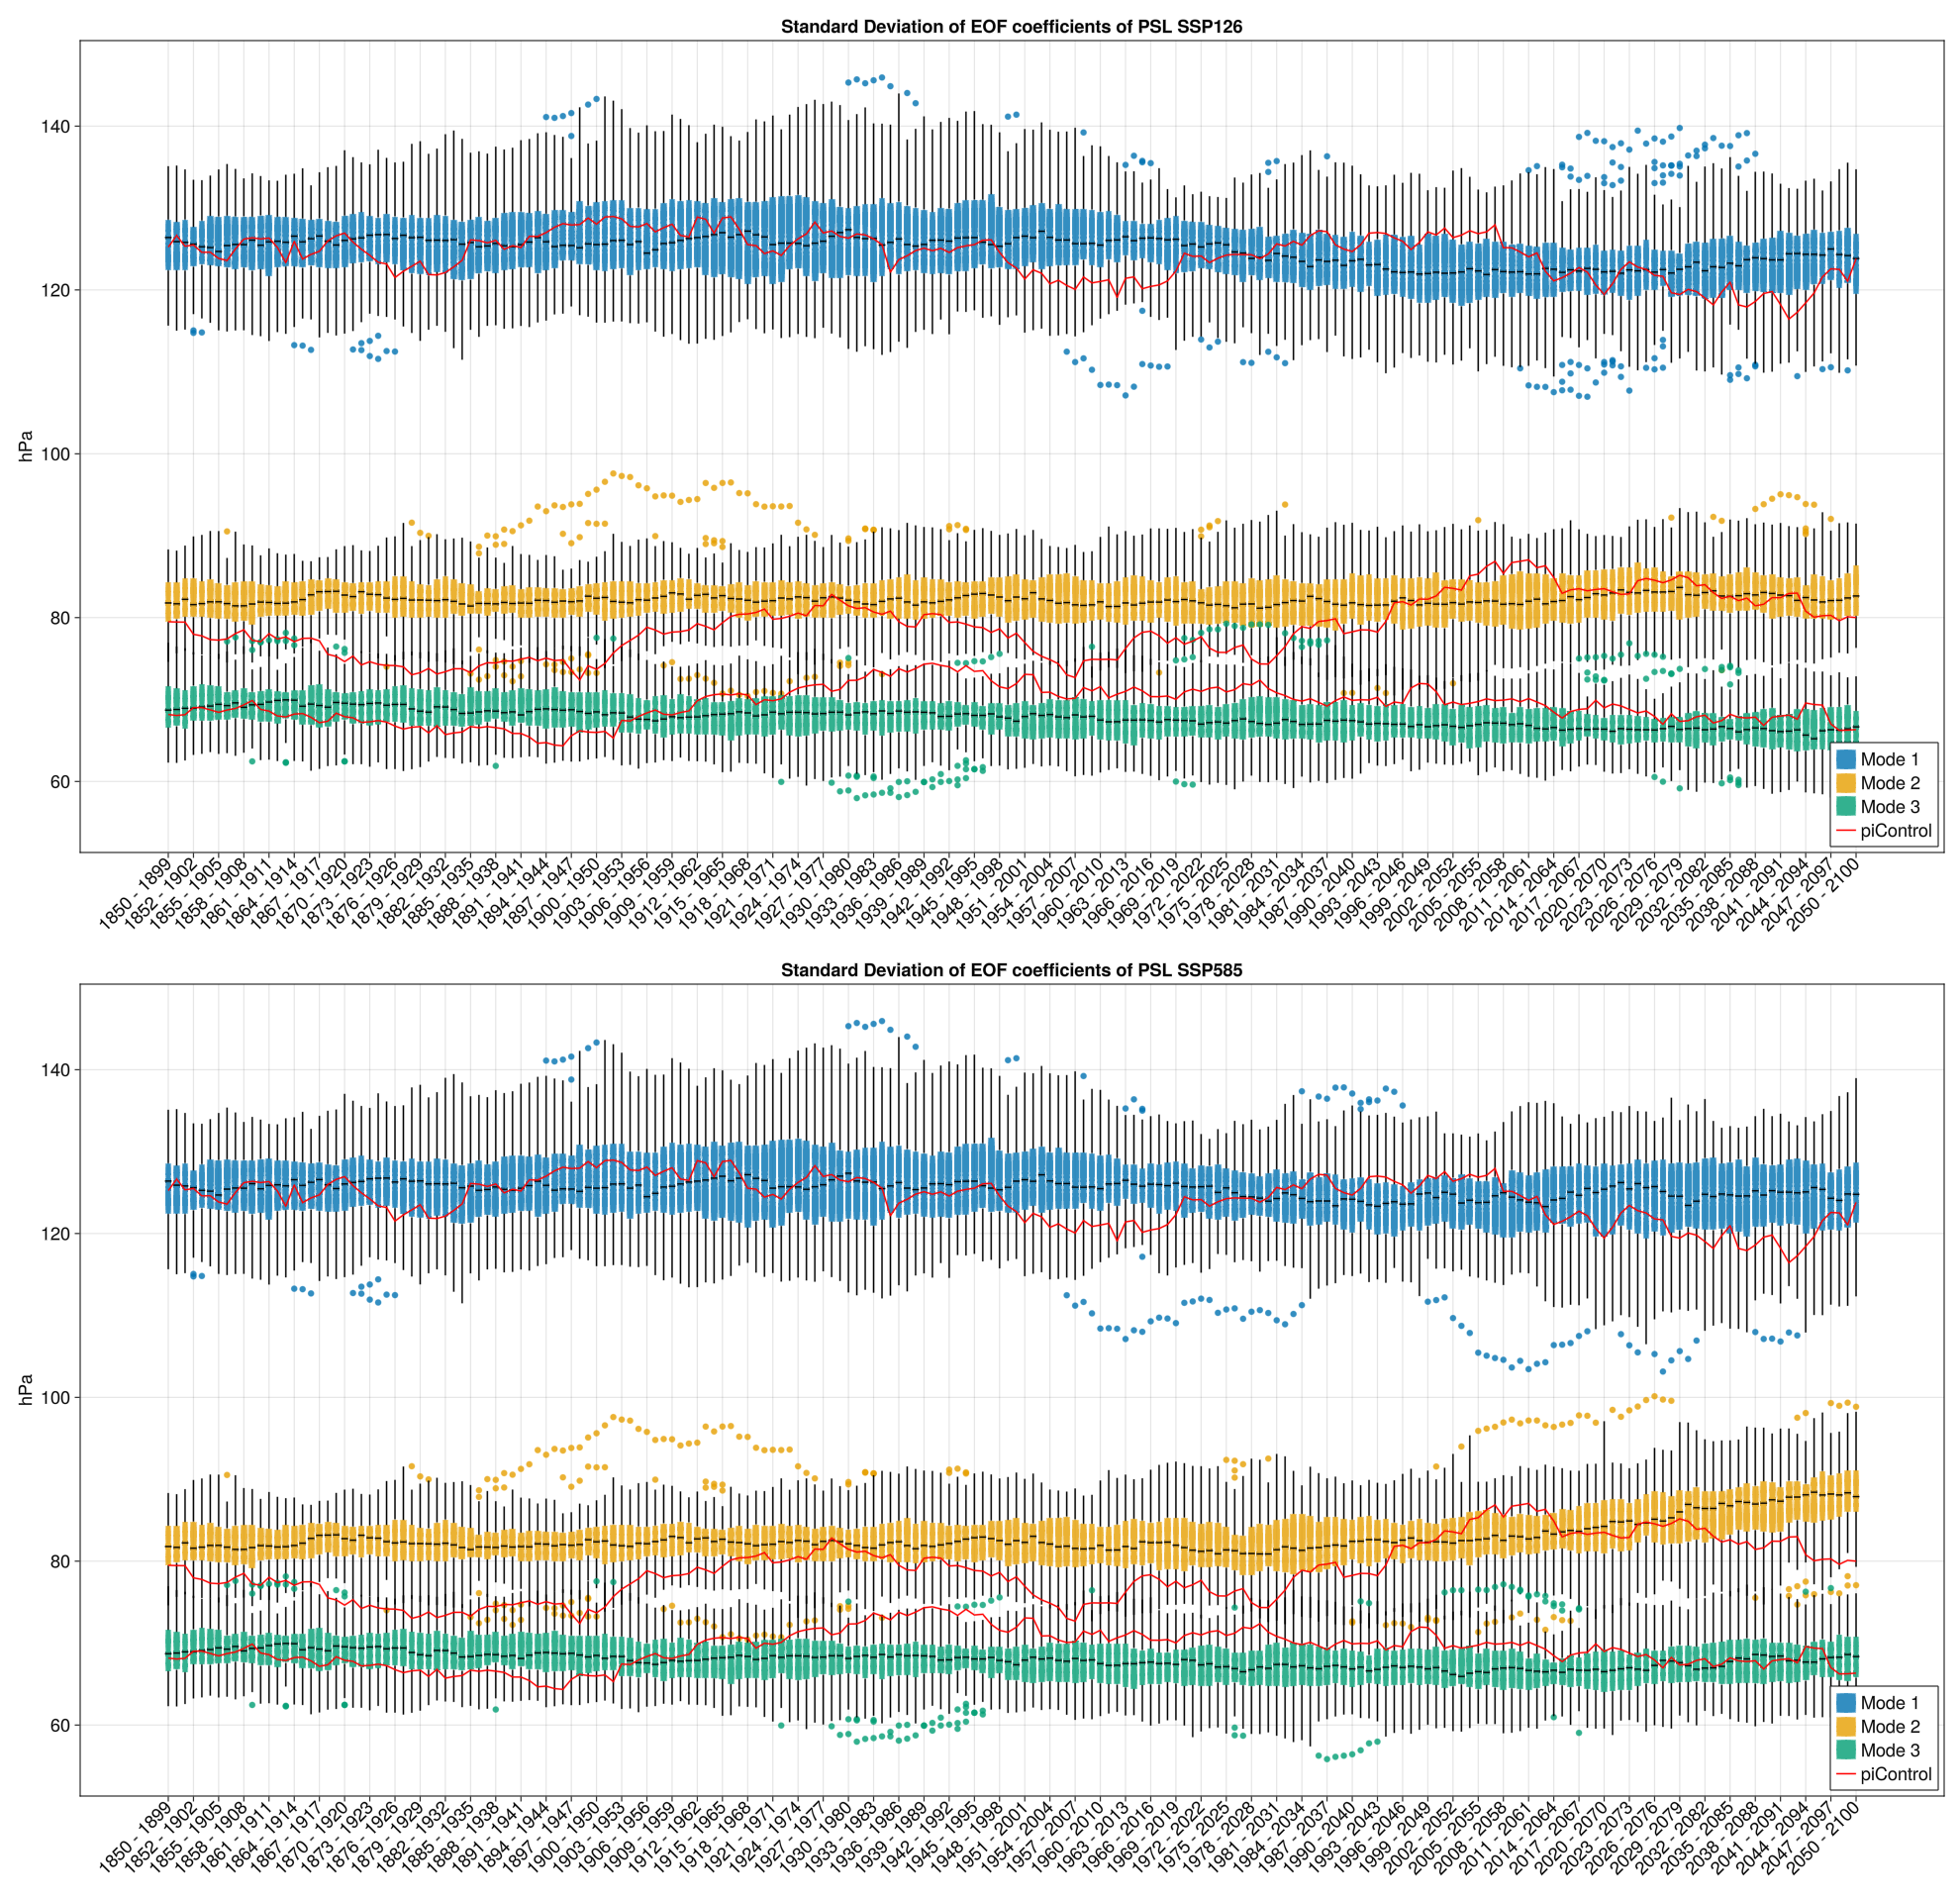
\includegraphics[width=0.65\textwidth]{figures/std_psl_50seasons_tempmodescale_3modes.png}
  \end{center}
  \caption{Same as Figure~\ref{fig:std ivt evolution}, but with sea level pressure data.}
  \label{fig:std psl evolution}
\end{figure}

Analyzing the evolution of the standard deviation of the IVT EOF coefficients, that compared to the quasi-stationary preindustrial control simulation the SD increases significantly, regardless of scenario. 
While Mode one experiences a drop in SD in the scopes from $\approx$ 1933 to 1999 (start of the scope), the SD of the members keep steadily increasing. 
This increase is far more pronounced in the SSP585 scenario than in SSP126, culminating in a median SD of $\approx 970~kg~s^{-1} m^{-1}$ (compared to $\approx 820~kg~s^{-1}m^{-1}$ in SSP126). 
This change is far more extreme than the sole change of proportionate encoded variability shown in Figure~\ref{fig:ivt mode variability}. 
The variance across the members seems pretty similar in both scenarios. 
All of this applies to modes two and three as well: Slow but steady increase in SD, which stays consistent in SSP126 but experiences a sharp increase in the later scopes of SSP585.  



\begin{figure}[htb]
  \begin{center}
    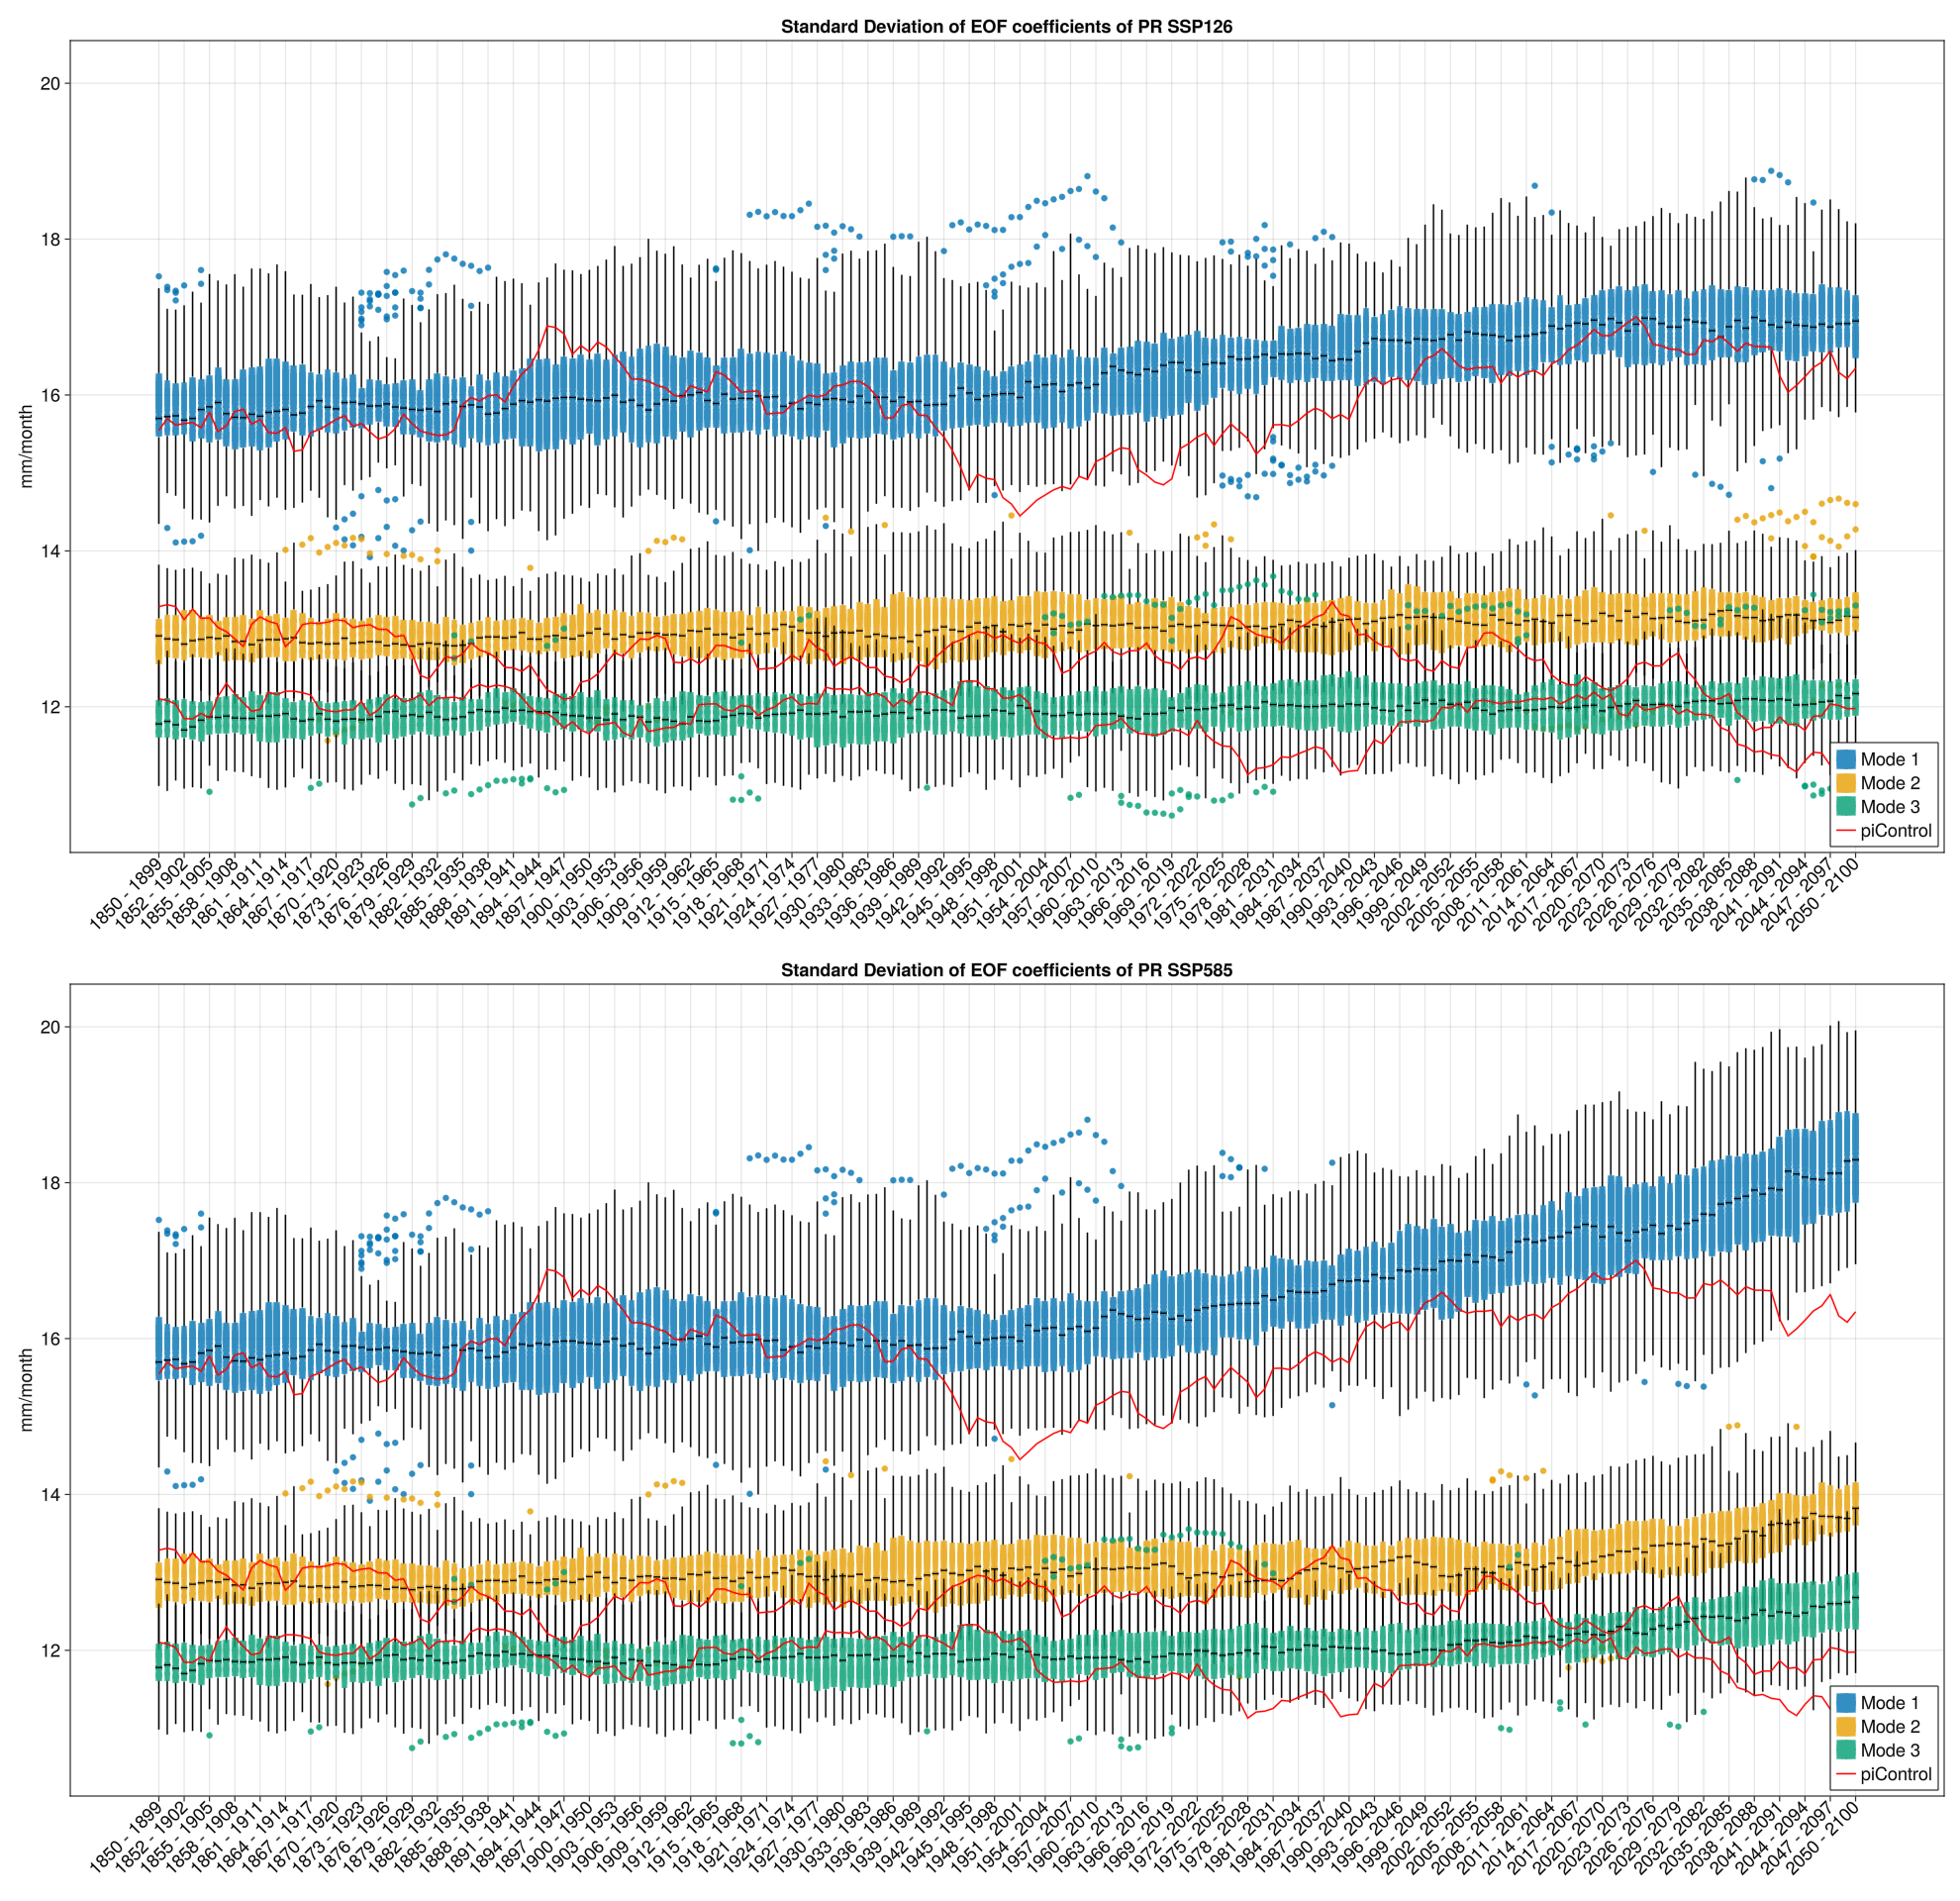
\includegraphics[width=0.65\textwidth]{figures/std_pr_50seasons_tempmodescale_3modes.png}
  \end{center}
  \caption{Same as Figure~\ref{fig:std ivt evolution}, but with precipitation data.}
  \label{fig:std pr evolution}
\end{figure}

Regarding the evolution of SD of sea level pressure EOF, it is obvious that the levels are more consistent over all the scopes, regardless of the scenario. 
Also, the piControl simulation is completely in line with the corresponding boxplots and could not be distinguished from the historical/scenario simulation. 
Comparing the scenarios, SD of Mode 1 coefficients (NAO indices) seem to be very similar to each other, with SSP585 having maybe a bit more variability across members. 
While it's also hard to distinguish the results of the different scenarios for Mode 3, SD evolution of Mode 2 (EAP indices) seem to experience a more pronounced increase in the later scopes in SSP585 than SSP126.  
This could be explained with the increase in proportional variability of that mode shown in Figure~\ref{fig:psl mode variability}.


The standard deviation of precipitation EOF coefficients seems to expose the largest differences in comparison to piControl simulation and the scenarios. 
Similarly to the IVT piControl EOF coefficients SD, the precipitation piControl has a dump in EOF coefficient SD in roughly the same timespan of scopes, which may be connected. 
The SSP126 scenario only shows a moderate increase in mode one, and no significant change in other modes. 
On the other hand, SSP585 shows a significant increase in all modes, which is different to the encoded variability shown in Figure~\ref{fig:pr mode variability}, where only the first mode exposes a steep increase. 



\section{Relationships with other Variables}

This section explores the correlation relationships between the dominant EOFs and other variables an their EOFs. 

\subsection{Relationships of EOFs}

The different EOFs of the variables can easily be compared by measuring the relationship between their temporal EOF coefficients. 
Although cross-correlation was used to find correlation patterns shifted in time (as explained in Section~\ref{sec:vis_analysis}), the analysis revealed that all somewhat correlated patterns had the highest correlation with lag zero ($\equiv$ same month). 
Therefore, finding the maximal cross-correlation distorts the actual correlation, which is expected to occur in the same month. 
That's why this section displays the not shifted correlation, while the analysis using cross correlation can be found in the appendix. \todo{Create Appendix!}
Following the argumentation in the previous section, only relationships between the first two modes of the variables were explored. 
Also, only the figures with significant correlations (Pearson Correlation $> 0.4$) are evaluated. 
Since the sample size is 200 ($50 \cdot 4$ months) for each scope, every result $> 0.5$ is significant at $p < 0.01$.


%
% \begin{figure}[htb]
%   \begin{center}
%     \subfloat[Caption for image 1]{
%         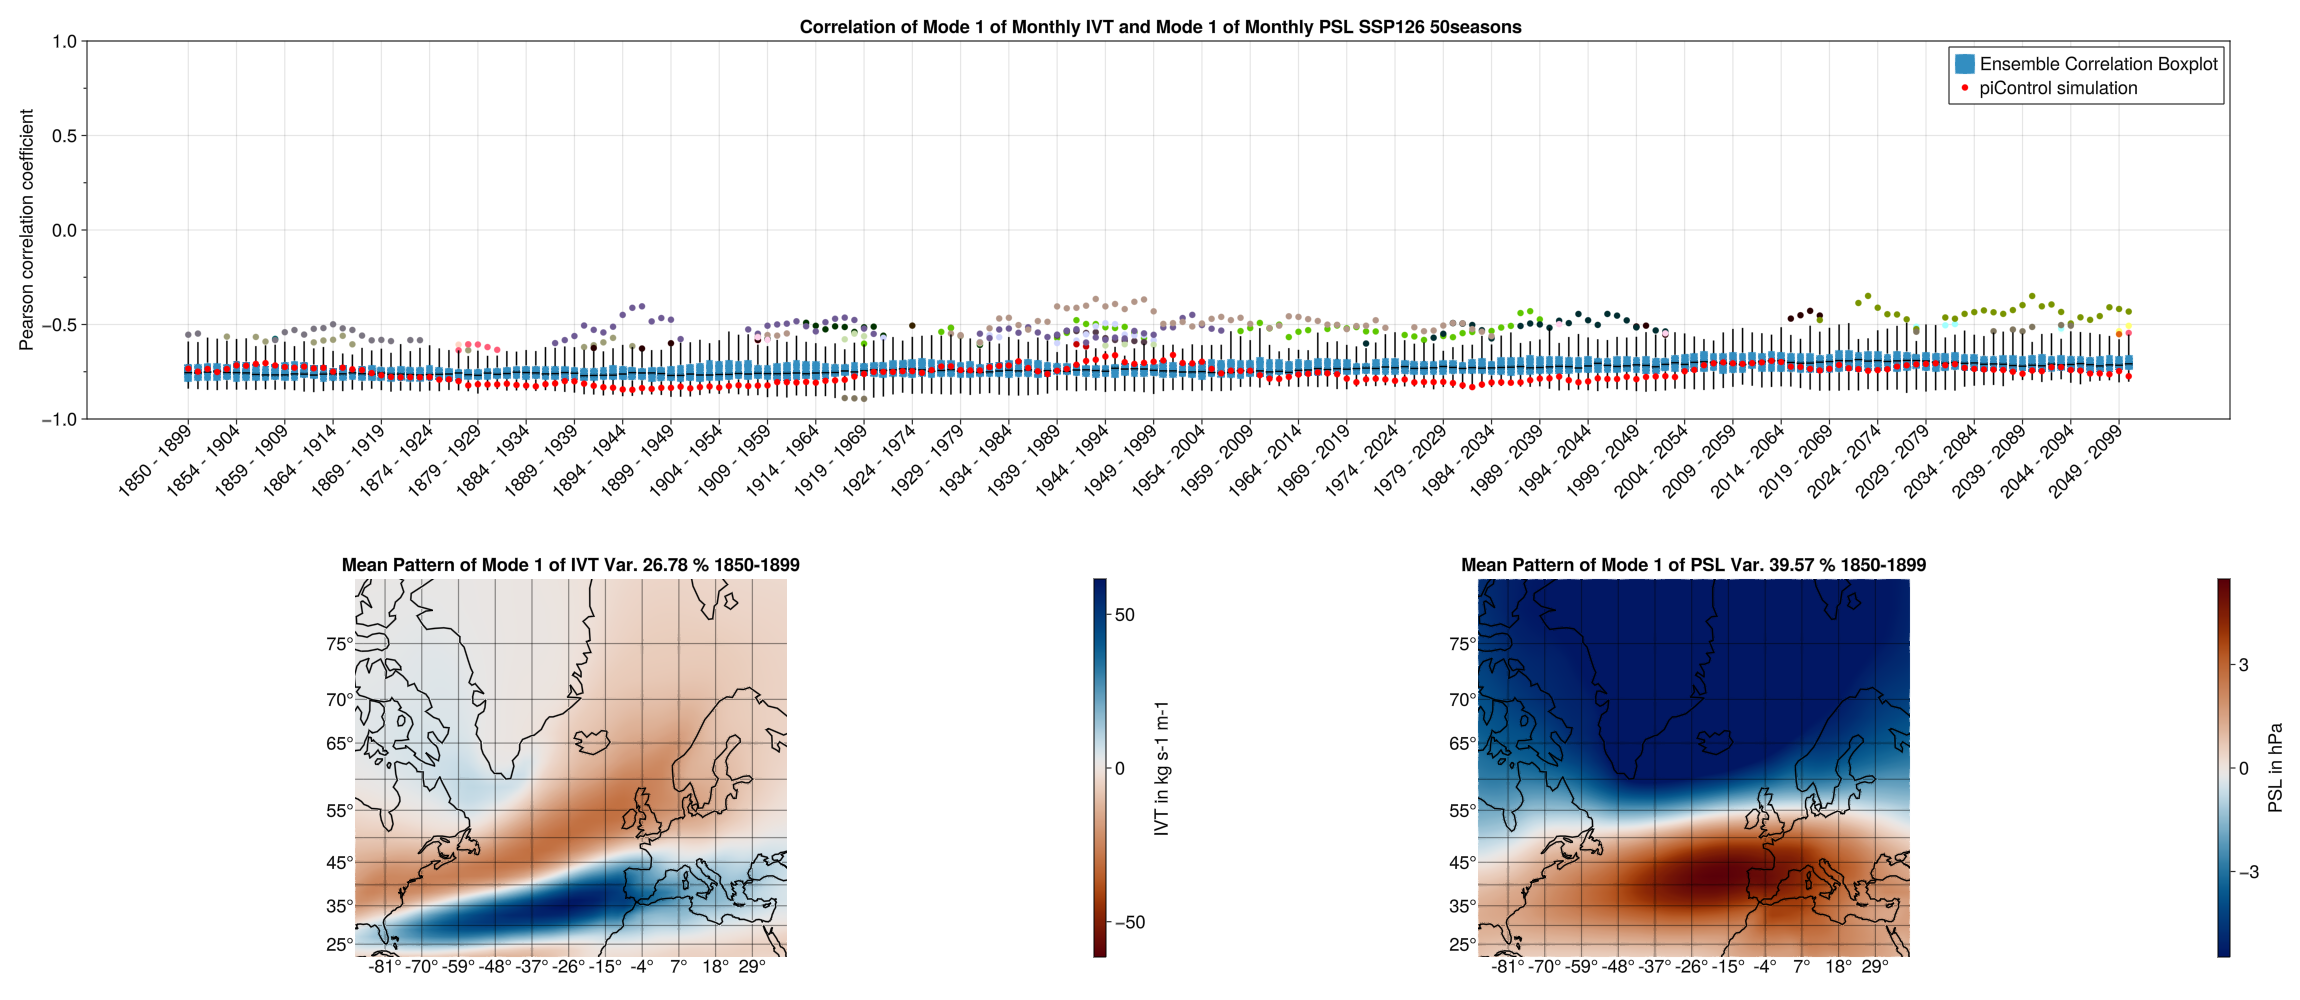
\includegraphics[width=0.49\textwidth]{figures/correlation_boxplot_ivt_psl_modes11_ssp126_50seasons.png}
%         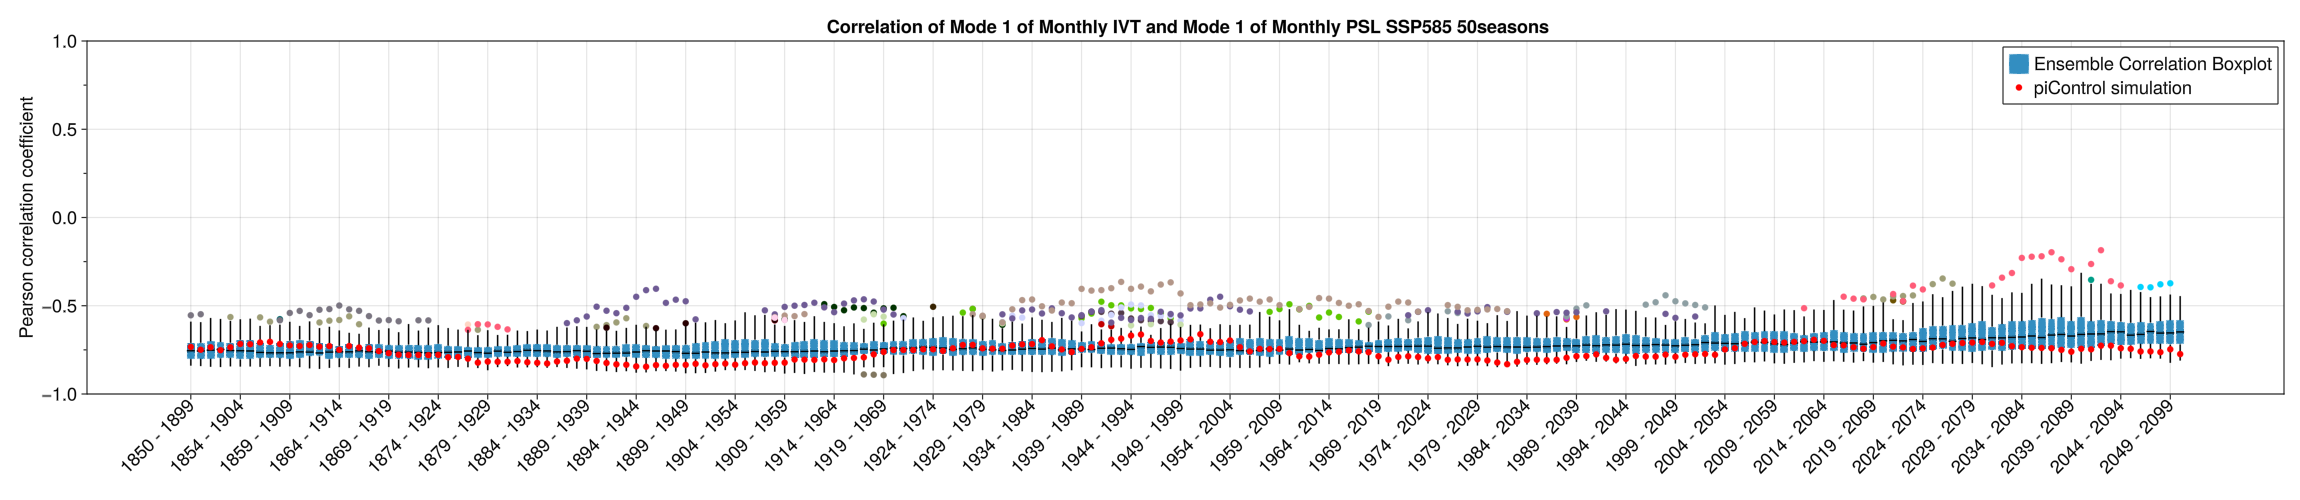
\includegraphics[width=0.49\textwidth]{figures/correlation_boxplot_ivt_psl_modes11_ssp585_50seasons.png}
%         \label{fig:image1}
%     }
%     \hfill
%     \subfloat[Caption for image 2]{
%         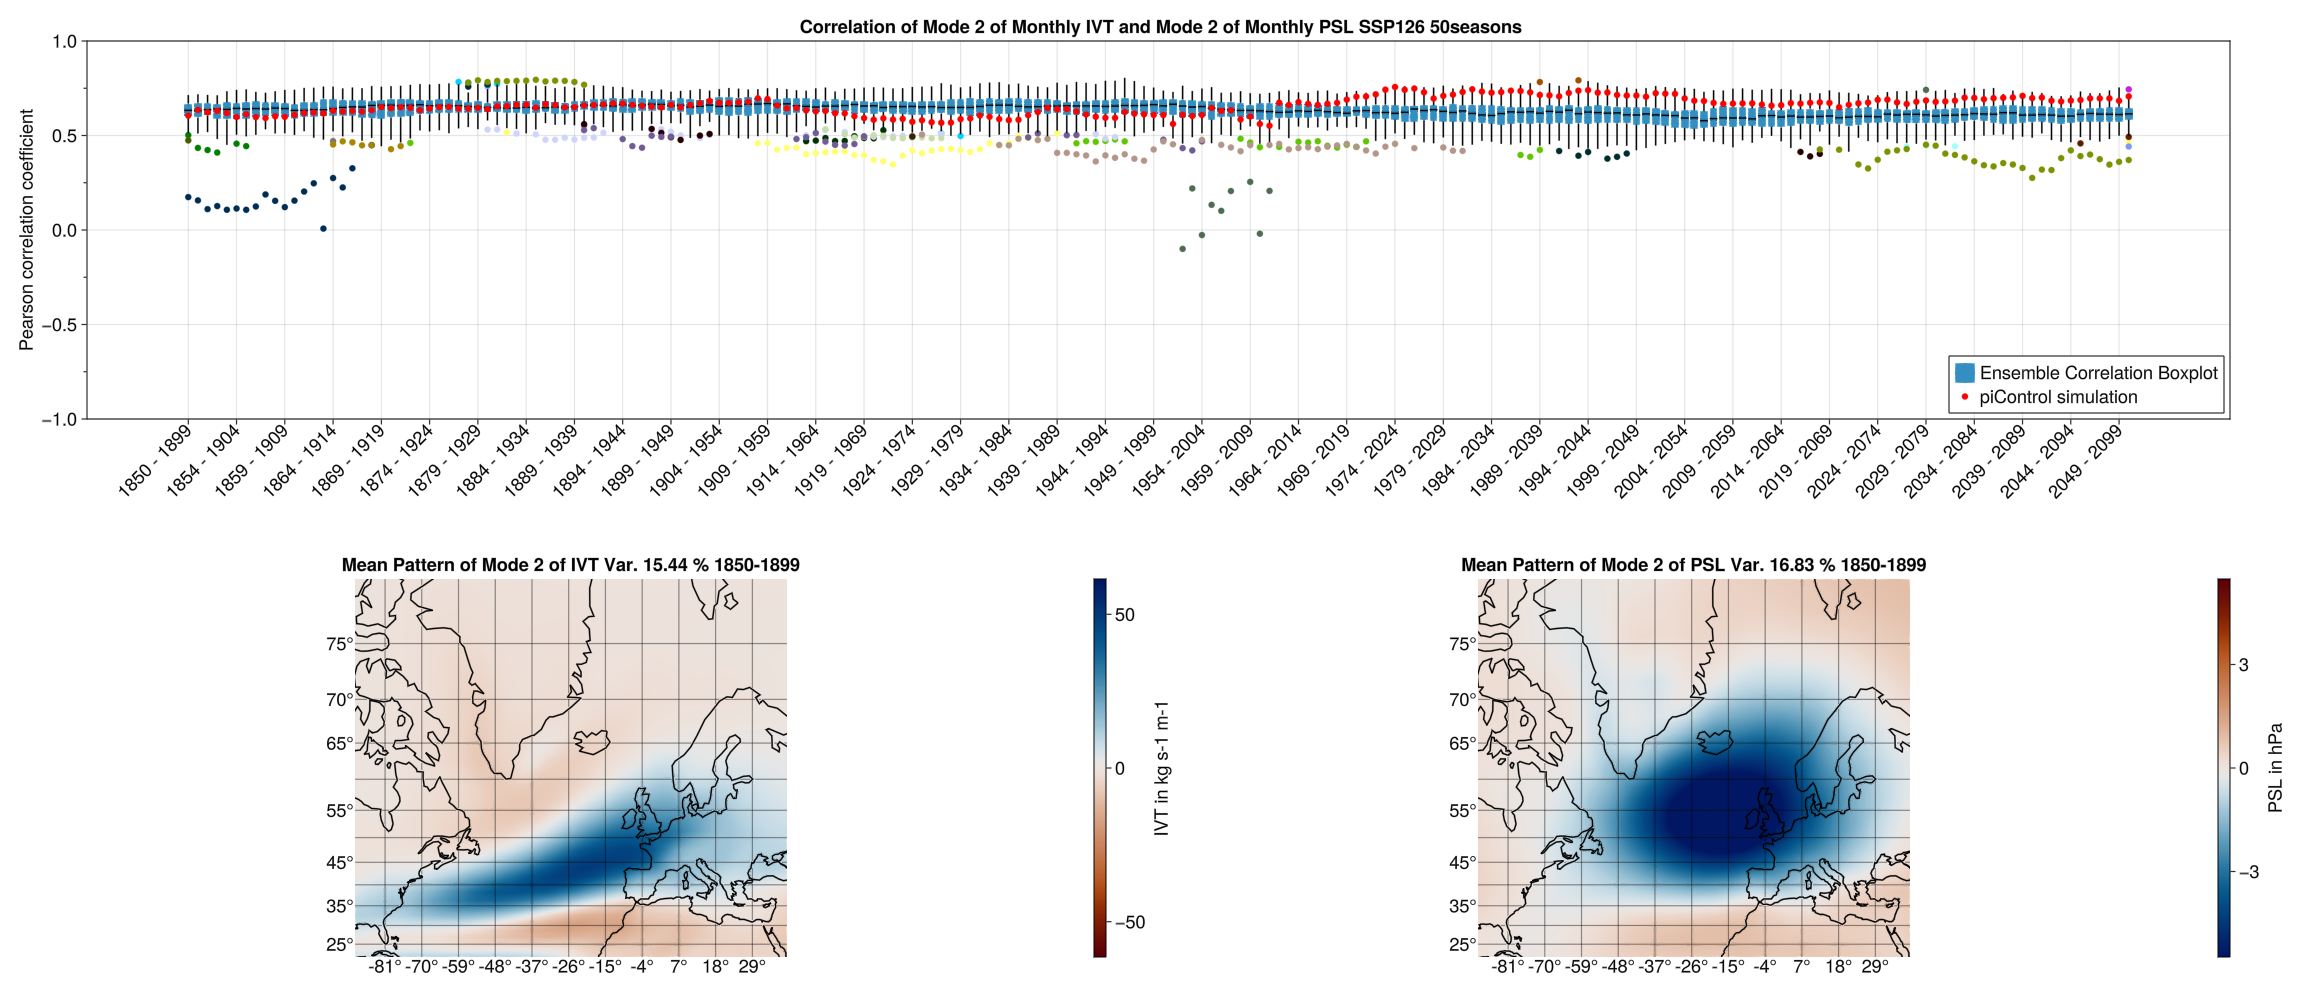
\includegraphics[width=0.49\textwidth]{figures/correlation_boxplot_ivt_psl_modes22_ssp126_50seasons.png}
%         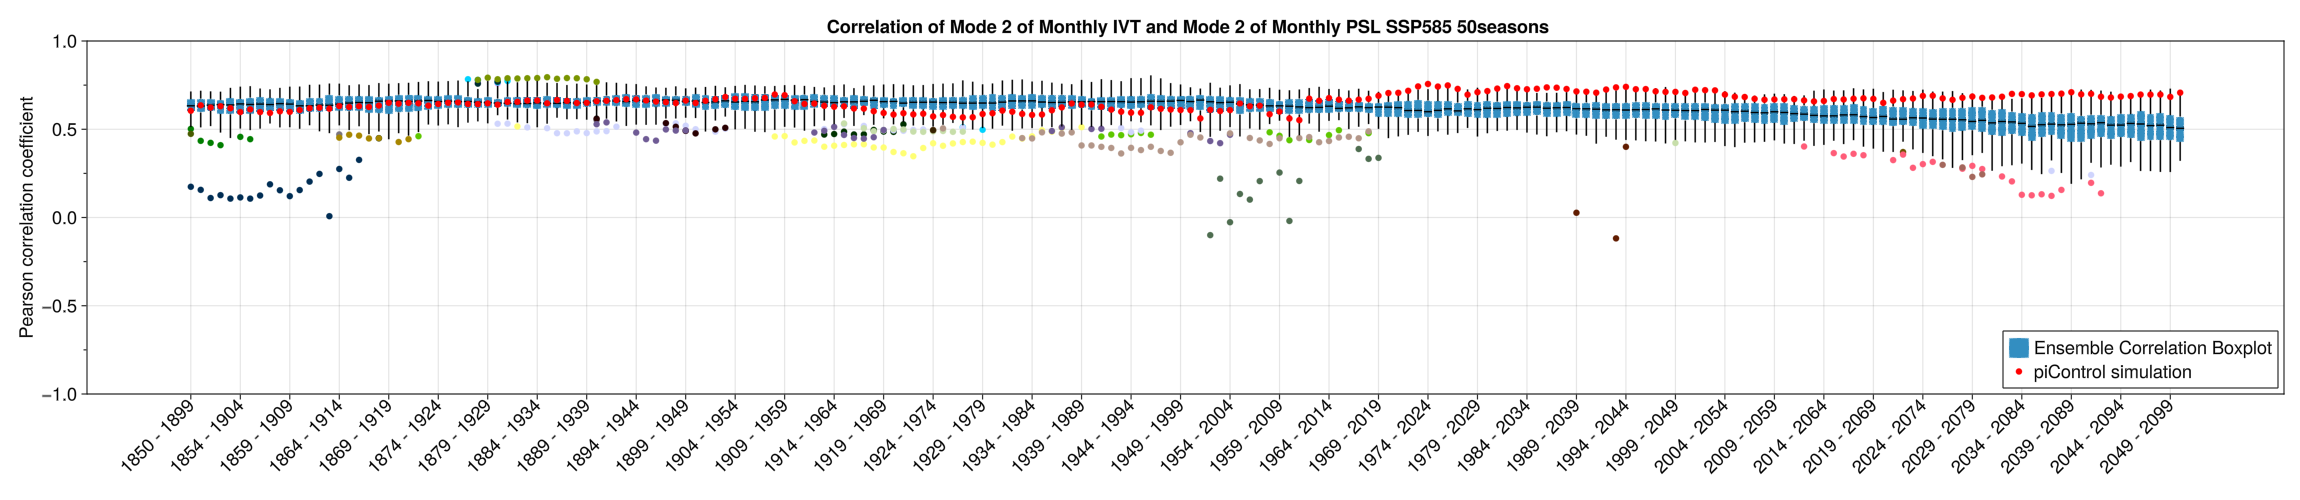
\includegraphics[width=0.49\textwidth]{figures/correlation_boxplot_ivt_psl_modes22_ssp585_50seasons.png}
%         \label{fig:image2}
%     }
%     
%   \end{center}
%   \caption{Correlation of Sea Level Pressure and IVT. Top row shows SSP126, bottom row SSP585. In the middle are images of the corresponding spatial patterns. The colors of the outliers refer to one specific member associated with that color.}
%   \label{fig:cor ivt psl modes11}
% \end{figure}
%

\begin{figure}[!tbp]
  \begin{subfigure}[b]{0.49\textwidth}
        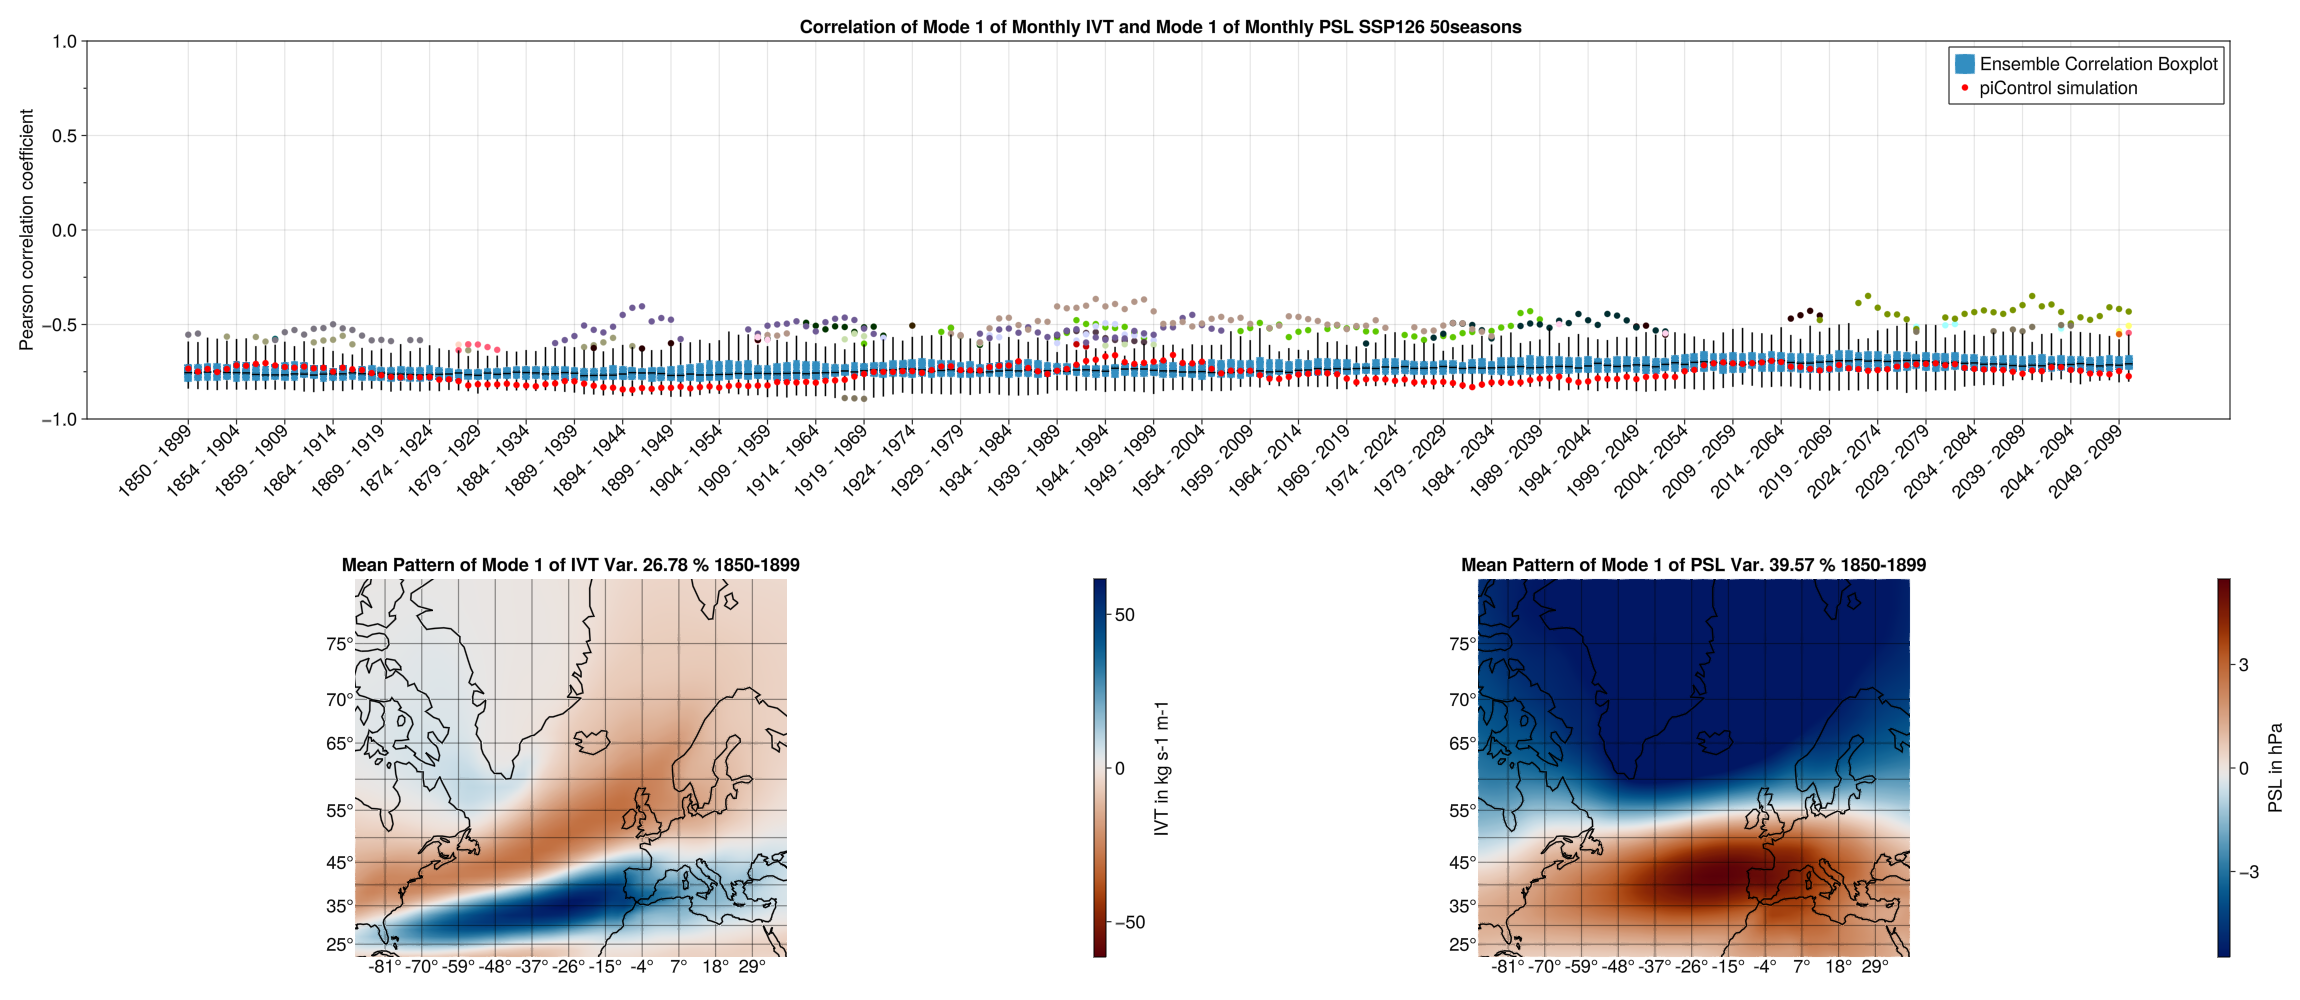
\includegraphics[width=\textwidth]{figures/correlation_boxplot_ivt_psl_modes11_ssp126_50seasons.png}
        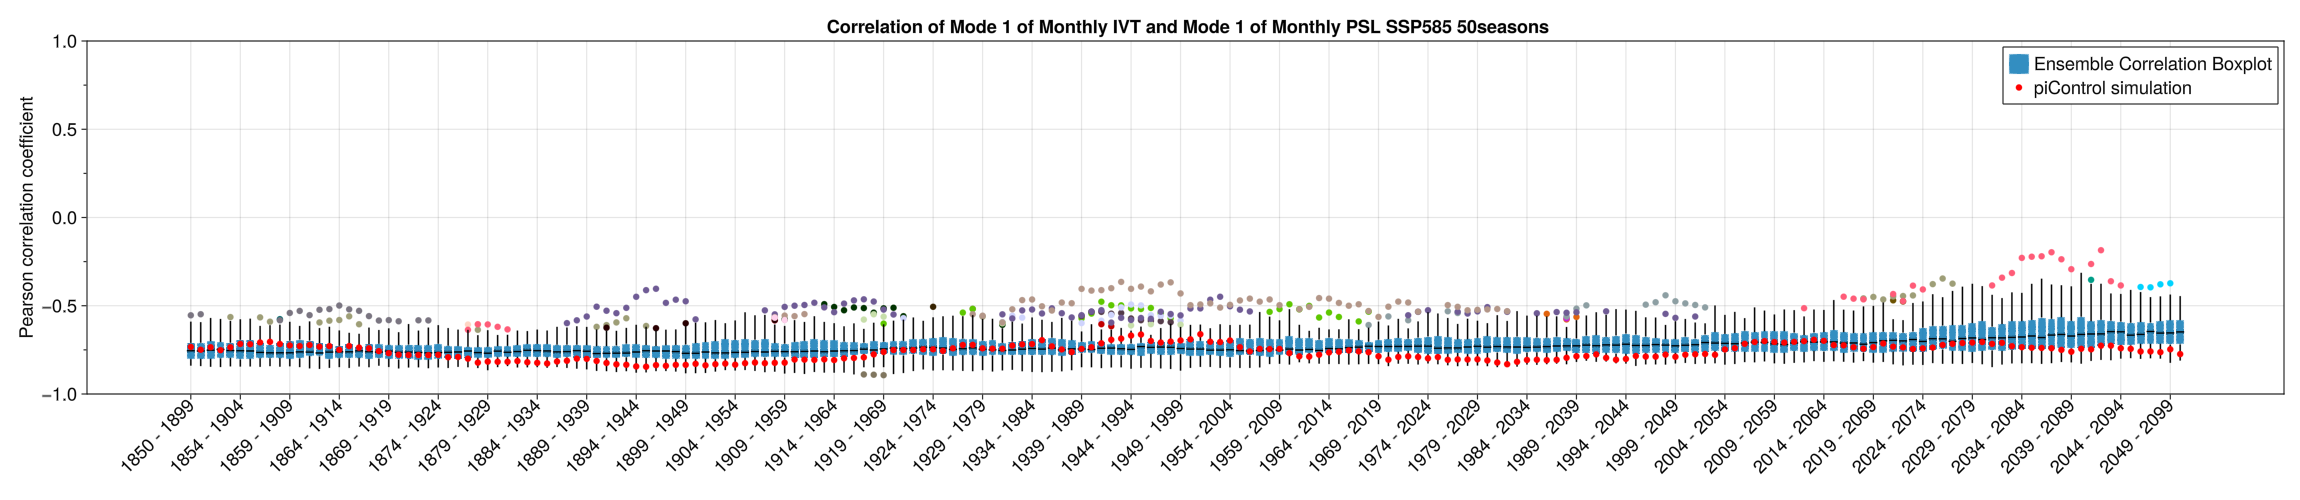
\includegraphics[width=\textwidth]{figures/correlation_boxplot_ivt_psl_modes11_ssp585_50seasons.png}
    \caption{Mode 1 of IVT and Mode 1 of PSL (NAO index)}
    \label{fig:cor ivt psl modes11}
  \end{subfigure}
  \hfill
  \begin{subfigure}[b]{0.49\textwidth}
        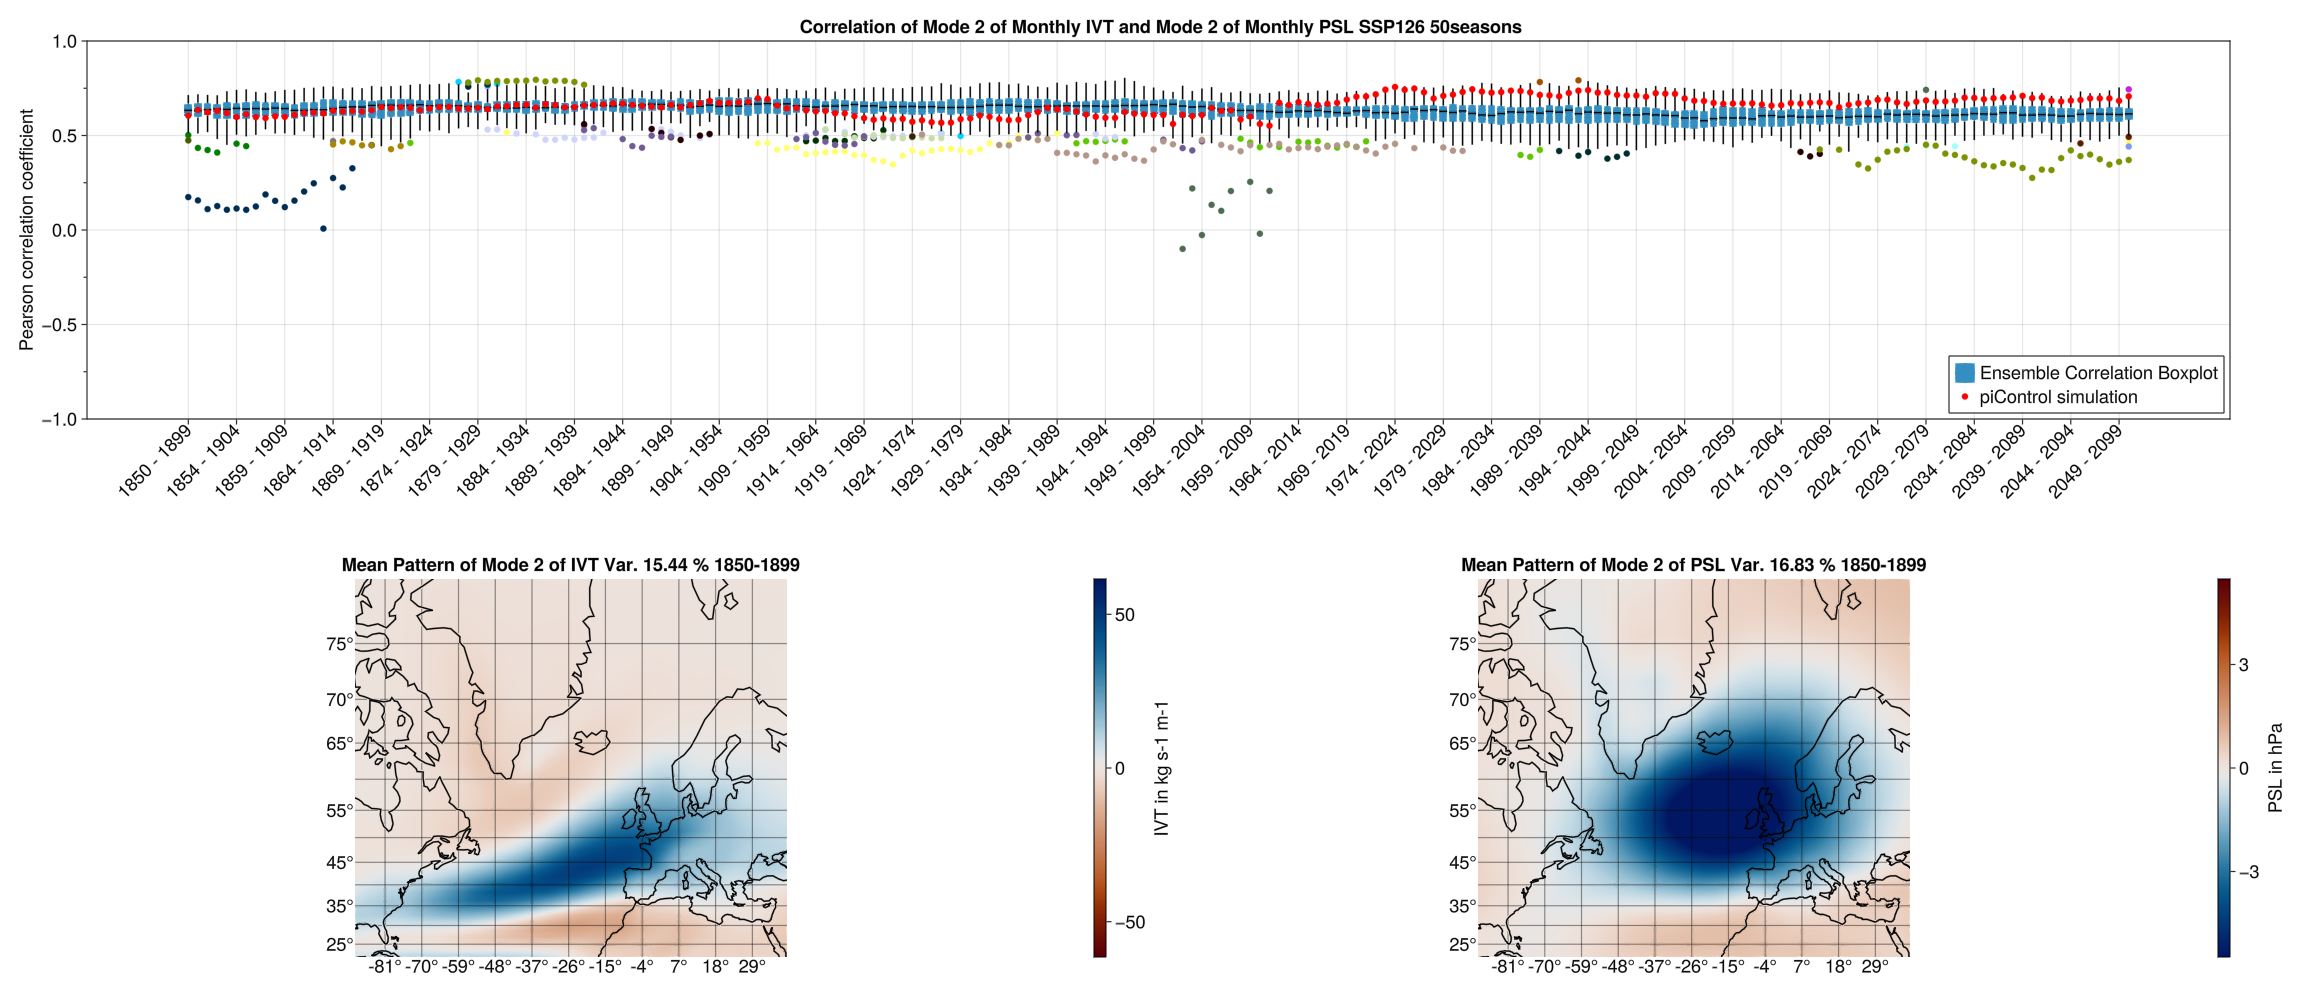
\includegraphics[width=\textwidth]{figures/correlation_boxplot_ivt_psl_modes22_ssp126_50seasons.png}
        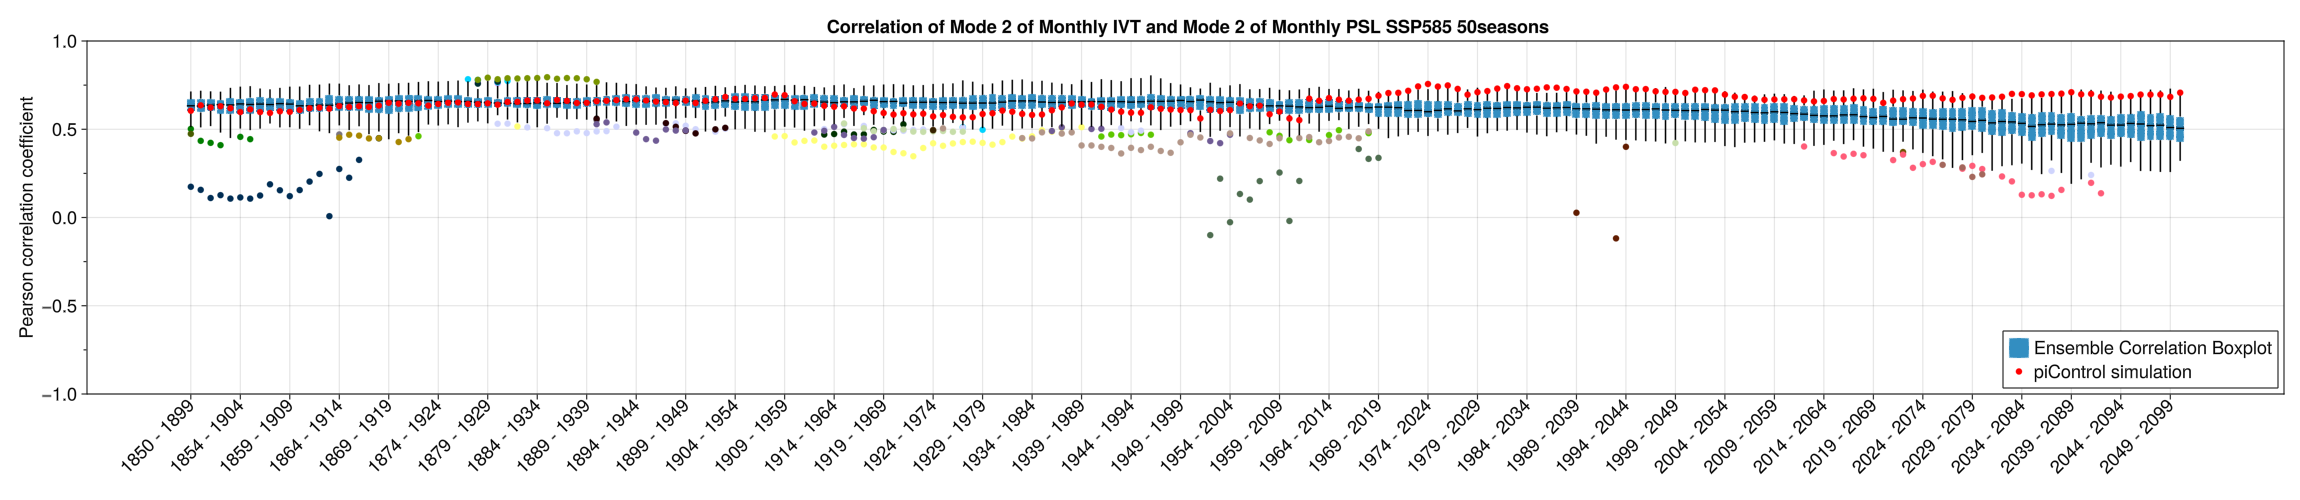
\includegraphics[width=\textwidth]{figures/correlation_boxplot_ivt_psl_modes22_ssp585_50seasons.png}
    \caption{Mode 2 of IVT and Mode 2 of PSL (EAP index)}
    \label{fig:cor ivt psl modes22}
  \end{subfigure}
  \caption{Correlation of Sea Level Pressure and IVT. Top row shows SSP126, bottom row SSP585. In the middle are images of the corresponding spatial patterns. The colors of the outliers refer to one specific member associated with that color.}
\end{figure}

The first relationships to explore are the ones between the indices of the dominant oscillations of the Atlantic and the IVT modes. 
In general, it is expected that high values of IVT are associated with low pressure areas.
Figure~\ref{fig:cor ivt psl modes11} shows the correlation of the NAO index with the activity of the primary IVT mode. 
As expected it shows a strong negative Pearson correlation coefficient (PCC) at about $-0.75$, with quite little variability across the different members. 
Comparing the different scenarios, it seems that SSP126 stays very similar to the historical simulation. 
SSP585 on the other hand seems to be more variable across the members and slightly less correlated in the later years. The first could be the reason for the latter. 

% \begin{figure}[htb]
%   \begin{center}
%     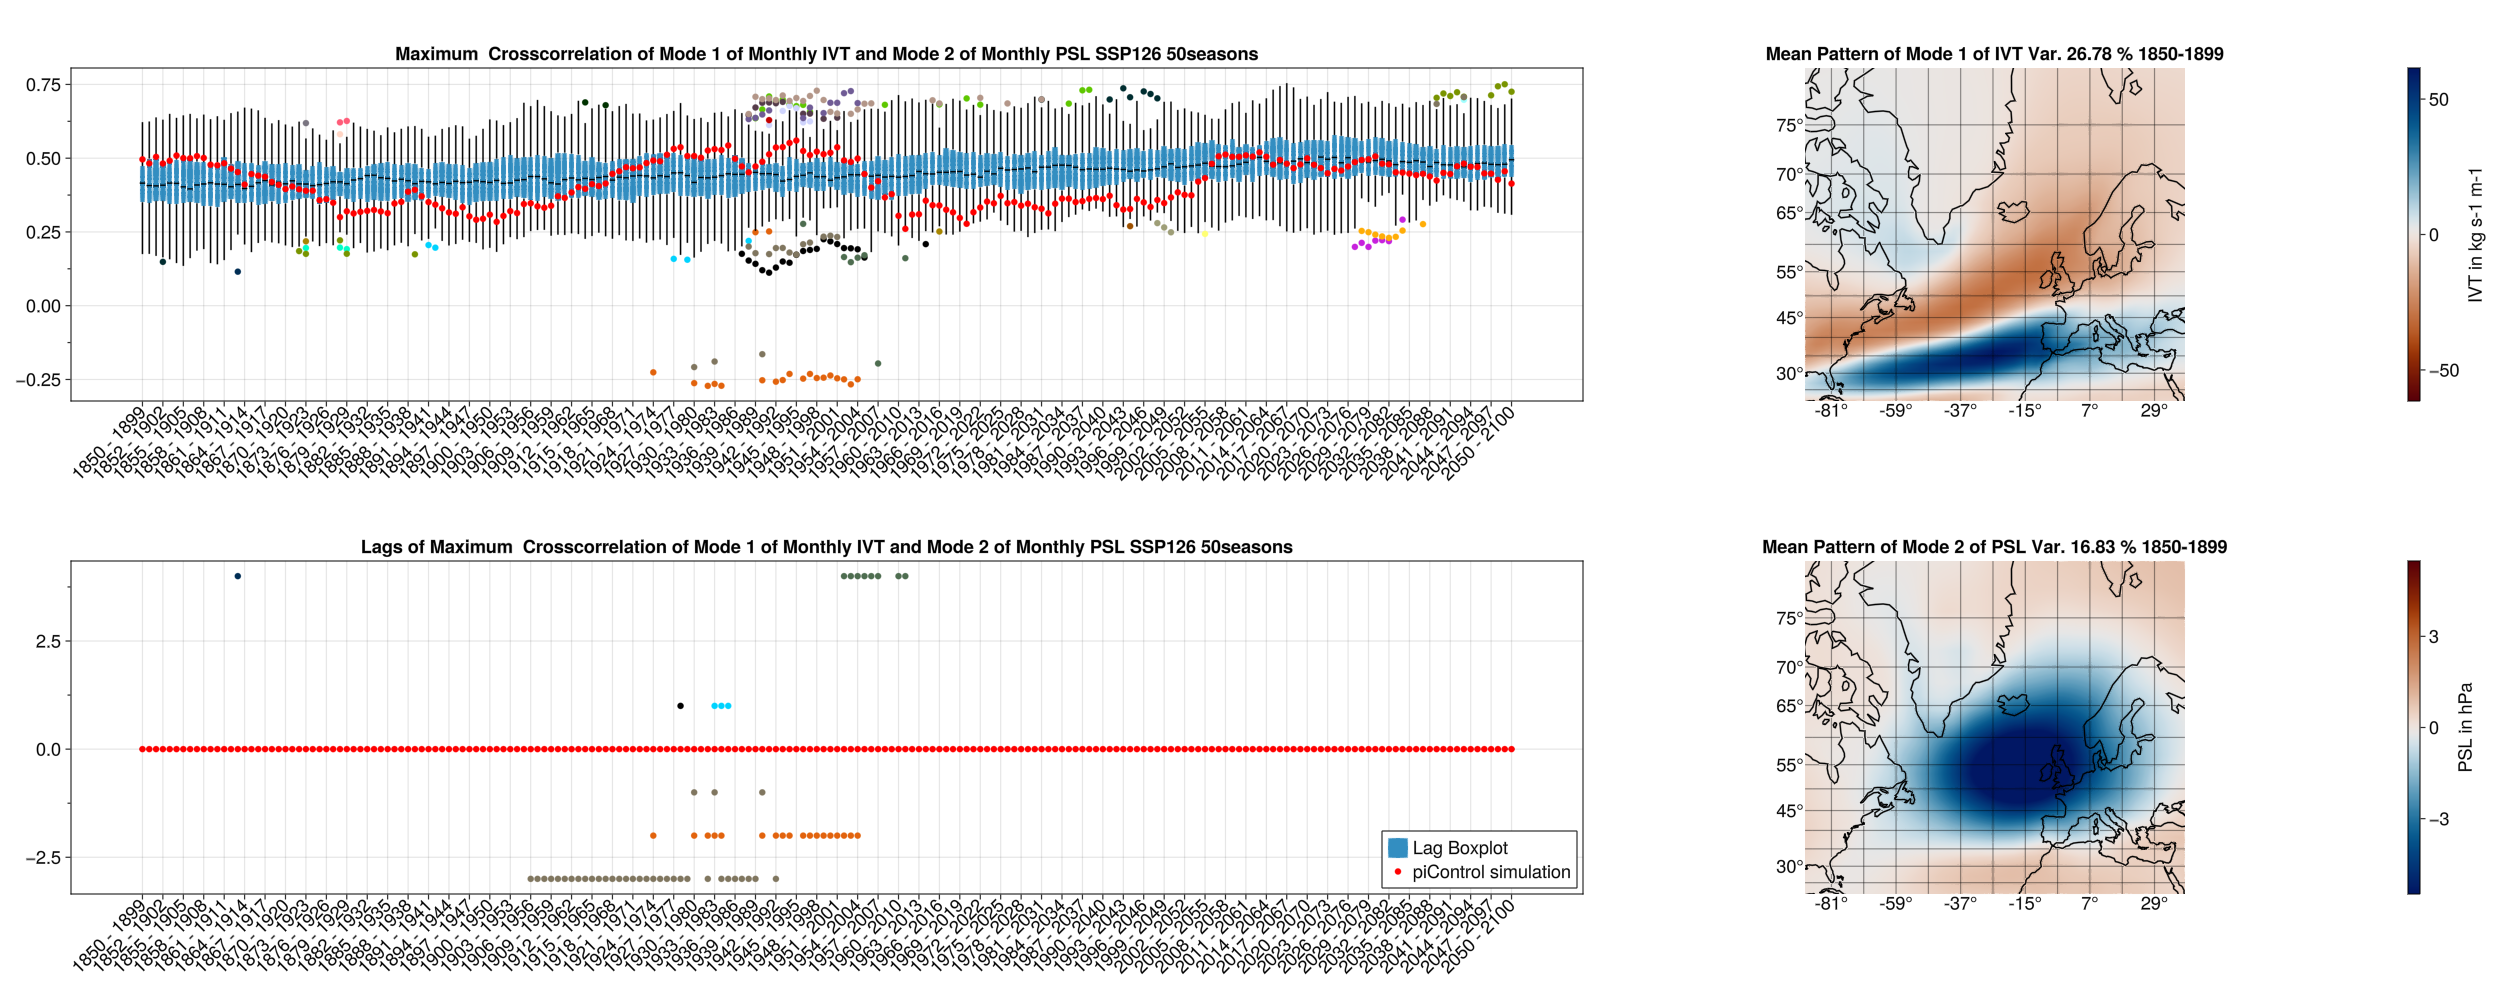
\includegraphics[width=0.95\textwidth]{figures/crosscorrelation_boxplot_ivt_psl_modes12_ssp126_50seasons.png}
%     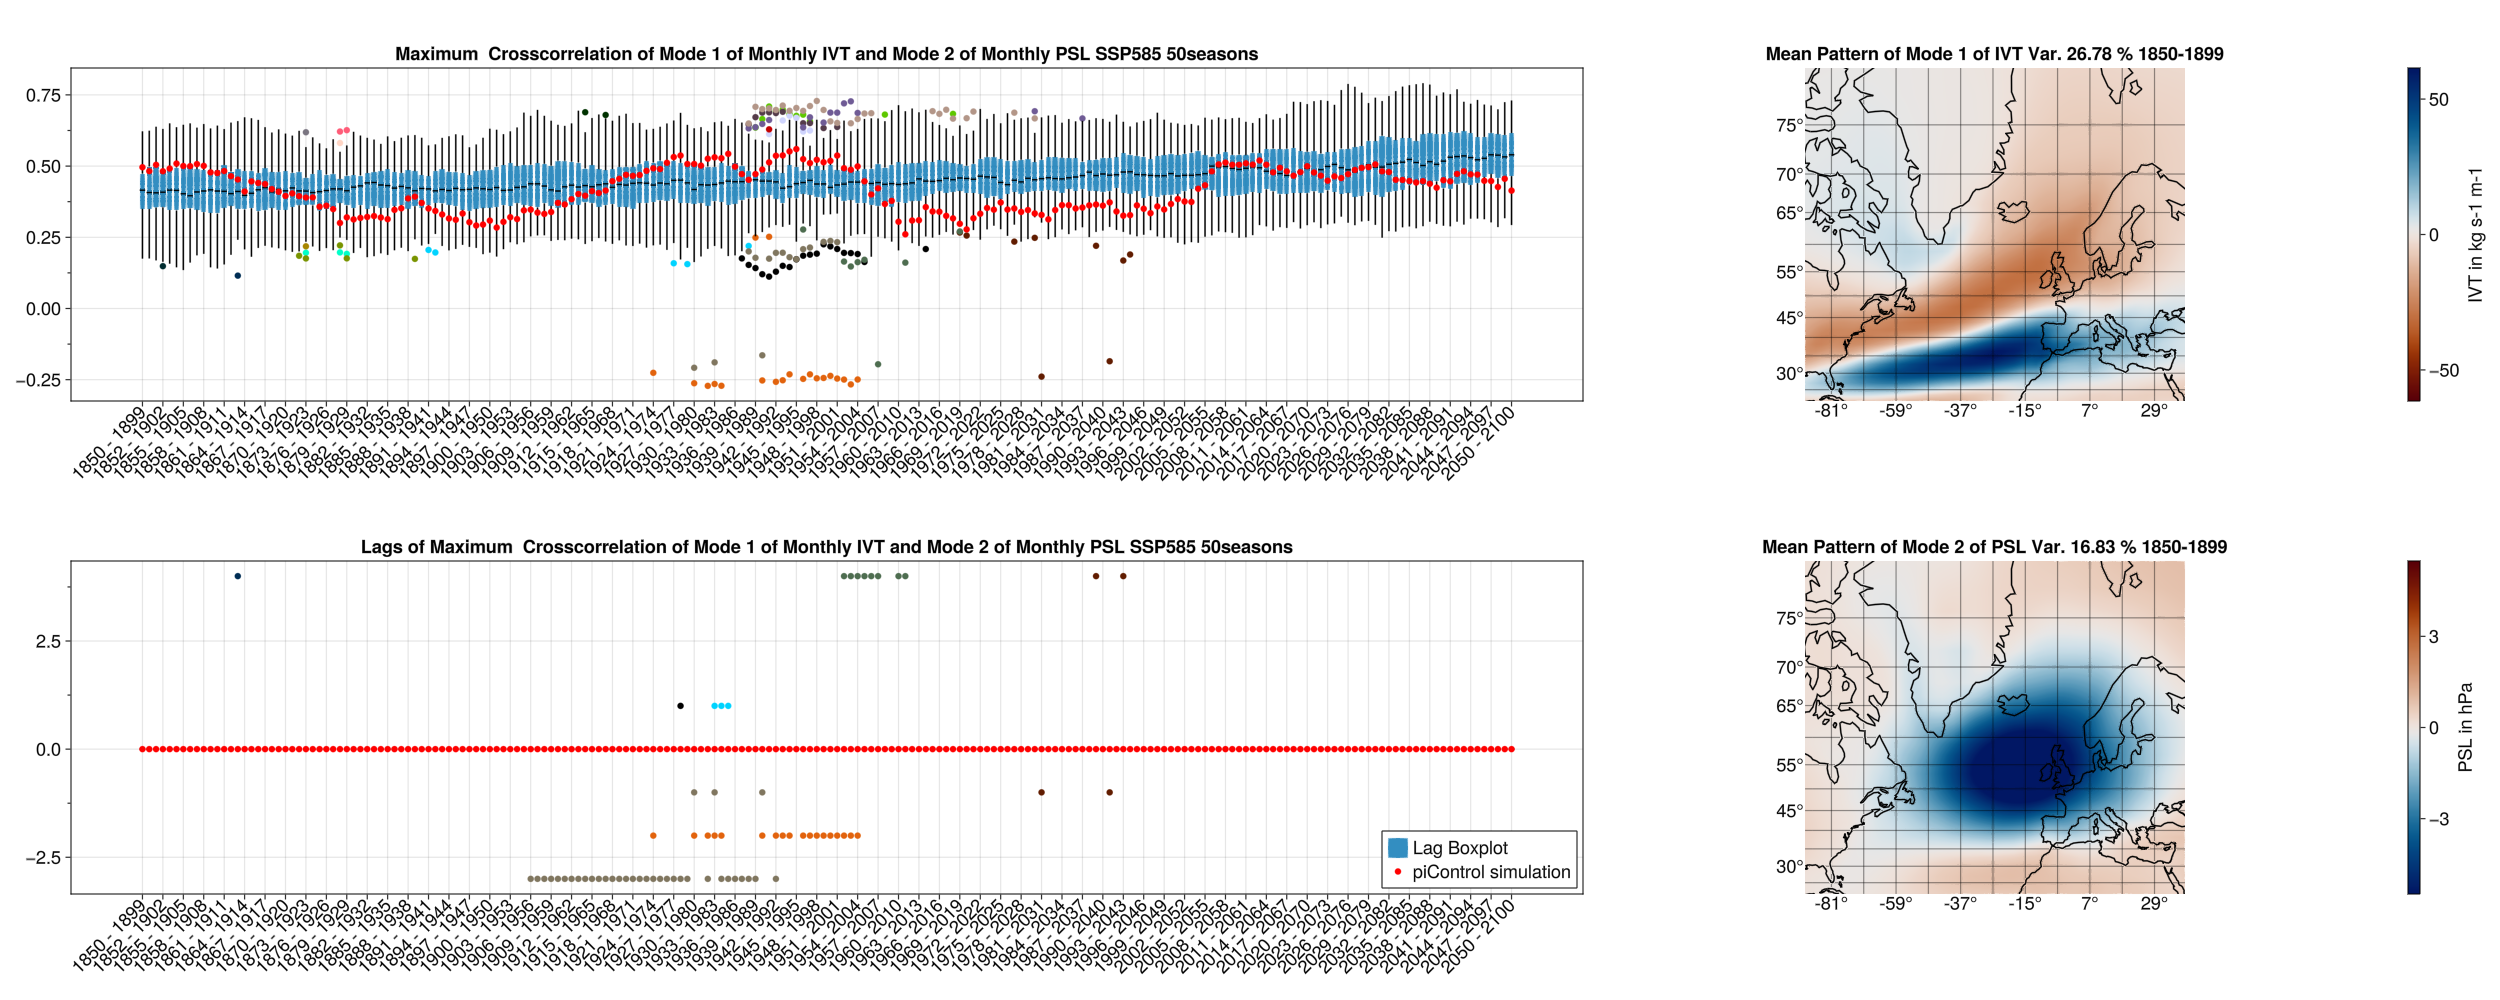
\includegraphics[width=0.95\textwidth]{figures/crosscorrelation_boxplot_ivt_psl_modes12_ssp585_50seasons.png}
%   \end{center}
%   \caption{Same as Figure~\ref{fig:cor ivt psl modes11}, but with mode 2 of Sea Level Pressure (EAP).}
%   \label{fig:crosscor ivt psl modes12}
% \end{figure}
%

The relationships between mode 1 and mode 2 of IVT and PSL and vice versa are pretty similar (Figure in the Appendix\todo{Figure in the Appendix}): 
Both have the media PCC around $0.5$, with the boxplots whiskers reaching around $0.25$. 
Also, both seem to experience a slight increase in median correlation in the late years of SSP585, while SSP126 stays pretty consistent. 




%
% \begin{figure}[htb]
%   \begin{center}
%   \end{center}
%   \caption{Same as Figure~\ref{fig:cor ivt psl modes11}, but with mode 2 of Sea Level Pressure (EAP) and IVT.}
%   \label{fig:cor ivt psl modes22}
% \end{figure}
%

Figure~\ref{fig:cor ivt psl modes22} shows the evolution of correlation of the index of the EAP with the secondary IVT mode. 
It shows a slightly weaker relationship than Figure~\ref{fig:cor ivt psl modes11} with a median PCC around $0.6$. 
Again, SSP126 stays similar to the historical simulation and the piControl simulation. 
But in SSP585, the correlation with the EAP index drops to a median of $0.5$, while the variability across members increases. 




\begin{figure}[!tbp]
  \begin{subfigure}[b]{0.49\textwidth}
    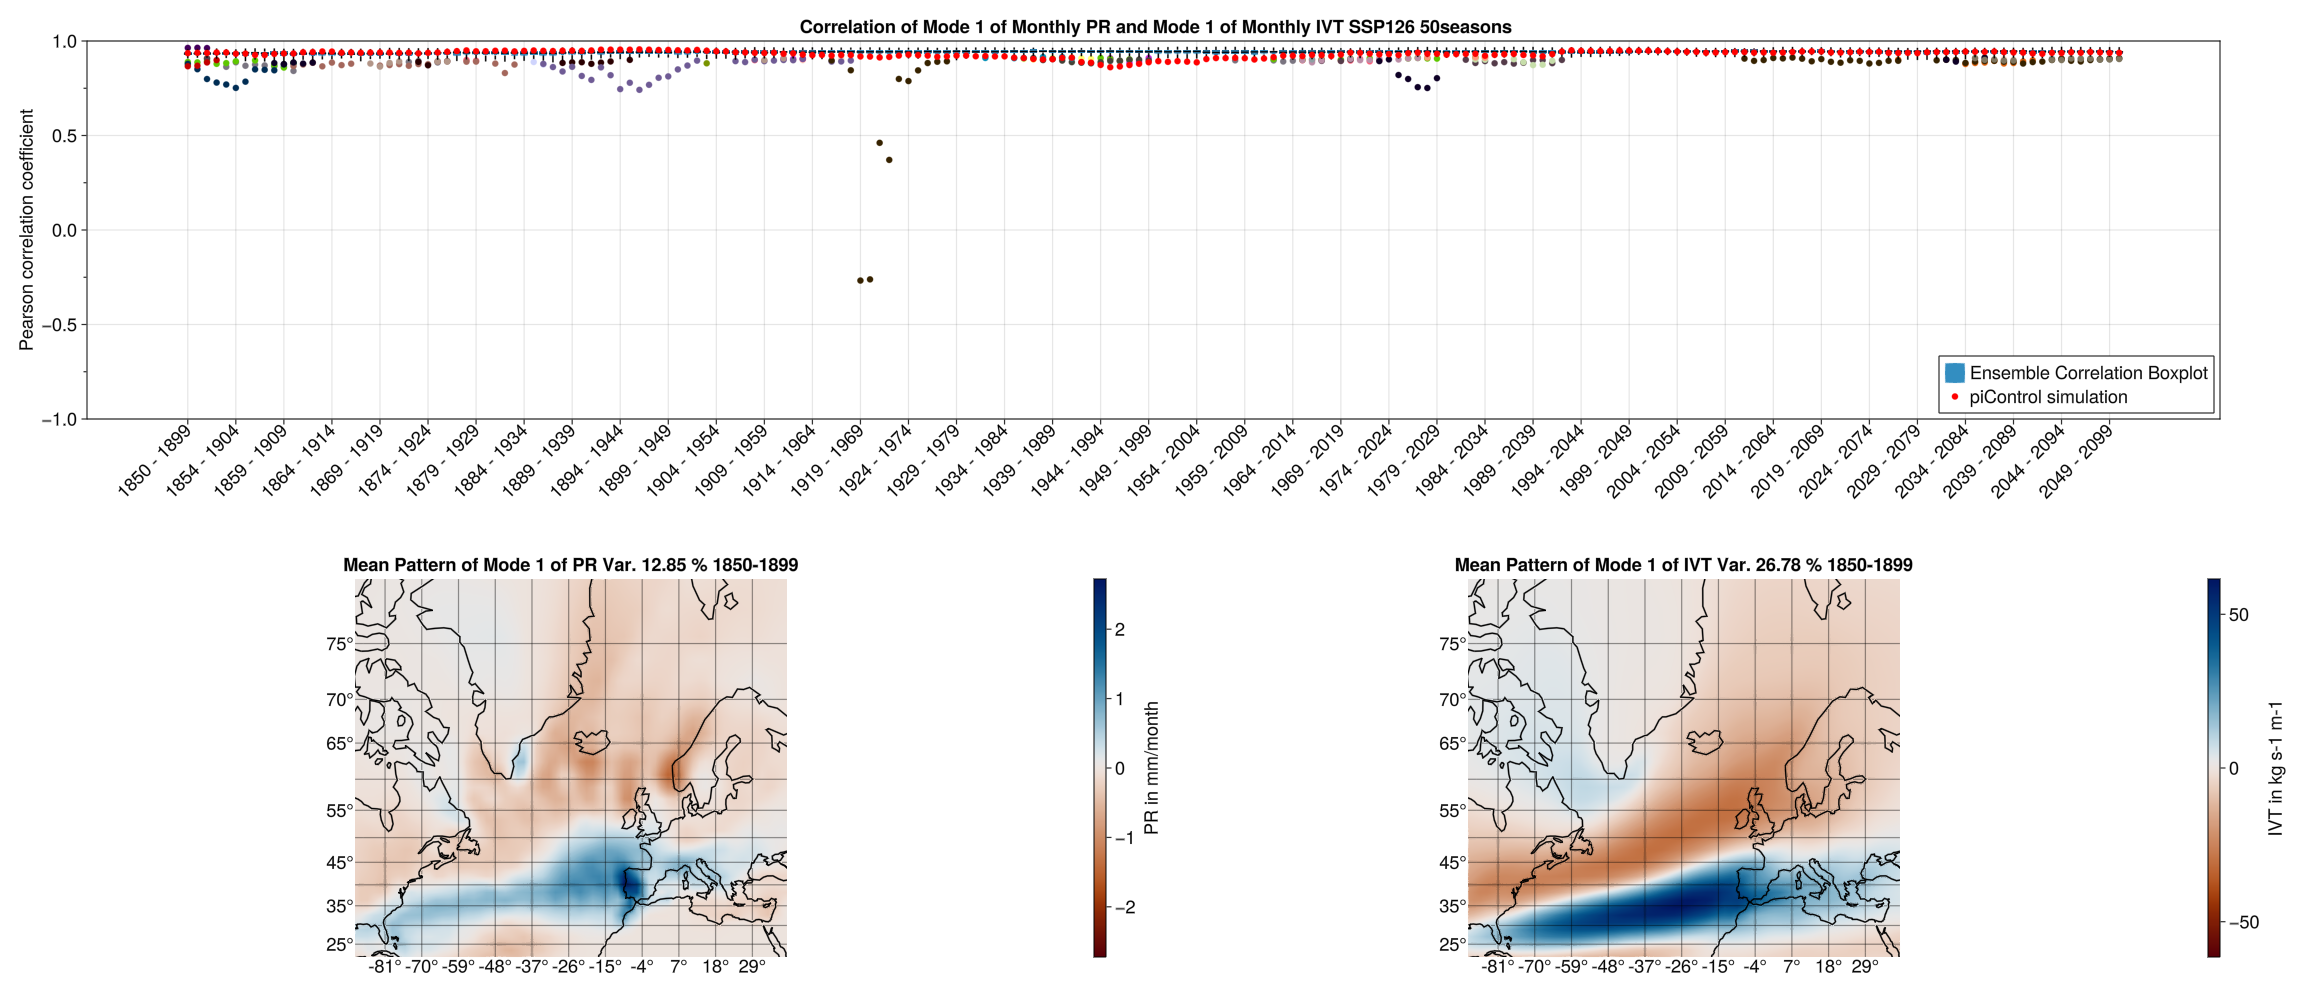
\includegraphics[width=\textwidth]{figures/correlation_boxplot_pr_ivt_modes11_ssp126_50seasons.png}
    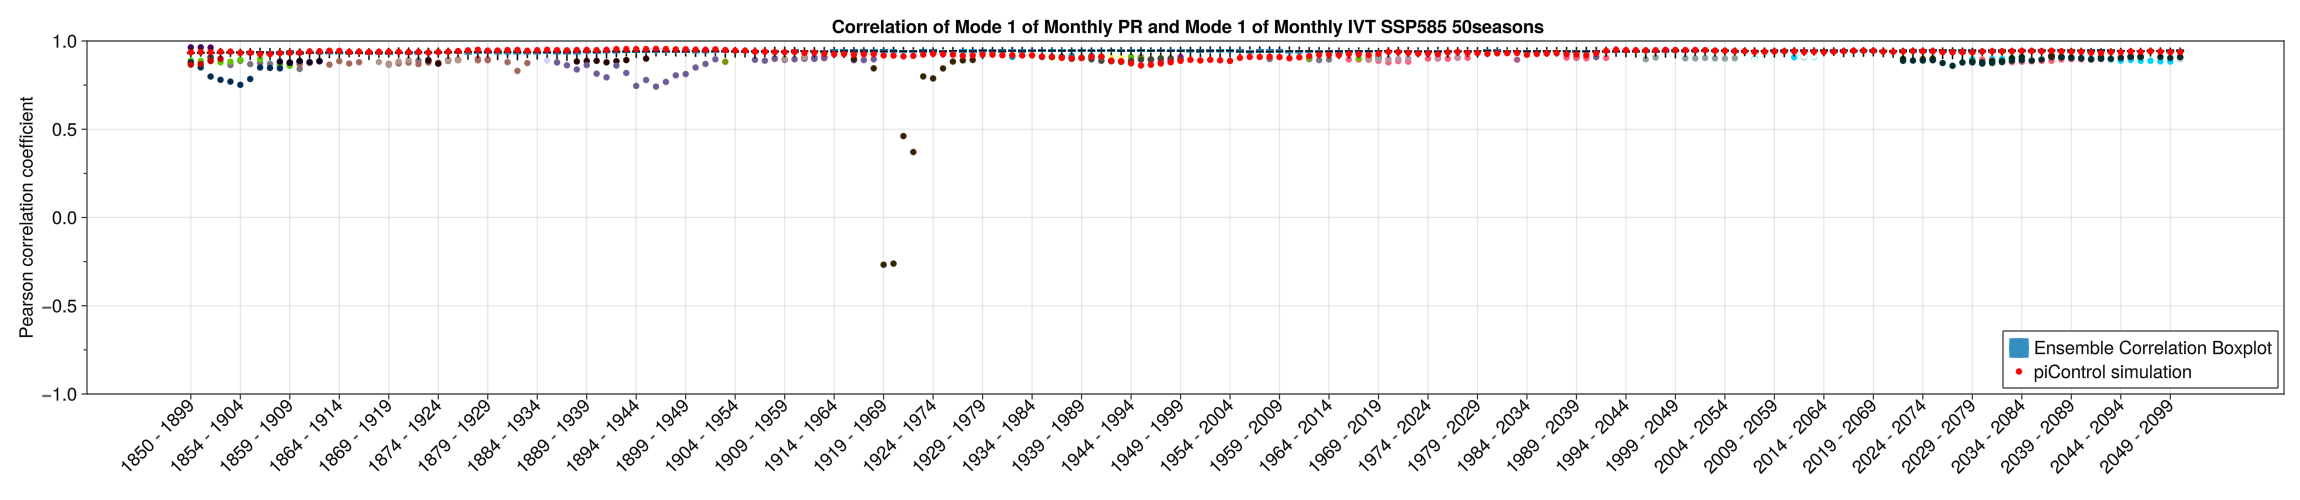
\includegraphics[width=\textwidth]{figures/correlation_boxplot_pr_ivt_modes11_ssp585_50seasons.png}
    \caption{Mode 1 of IVT and Mode 1 of precipitation}
    \label{fig:cor pr ivt modes11}
  \end{subfigure}
  \hfill
  \begin{subfigure}[b]{0.49\textwidth}
    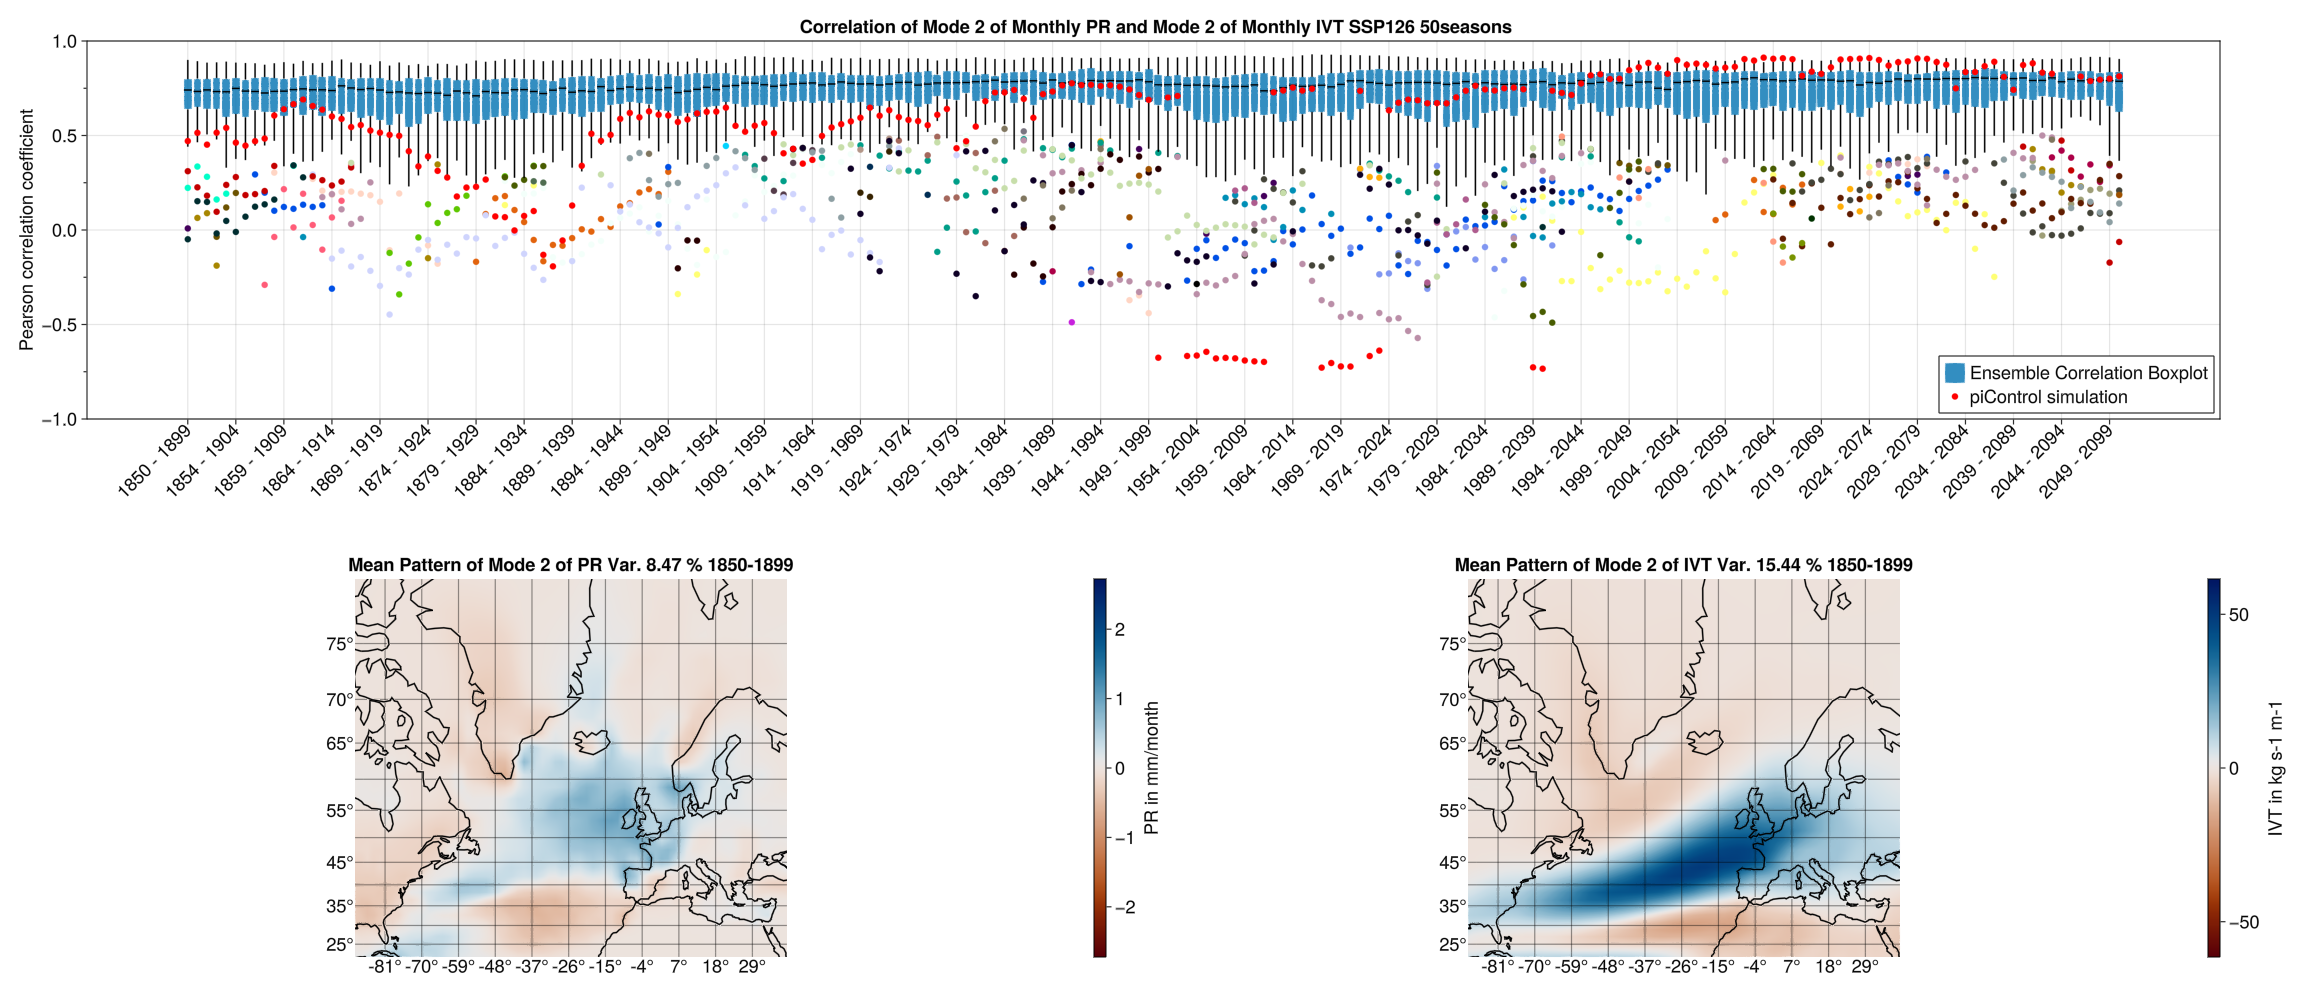
\includegraphics[width=\textwidth]{figures/correlation_boxplot_pr_ivt_modes22_ssp126_50seasons.png}
    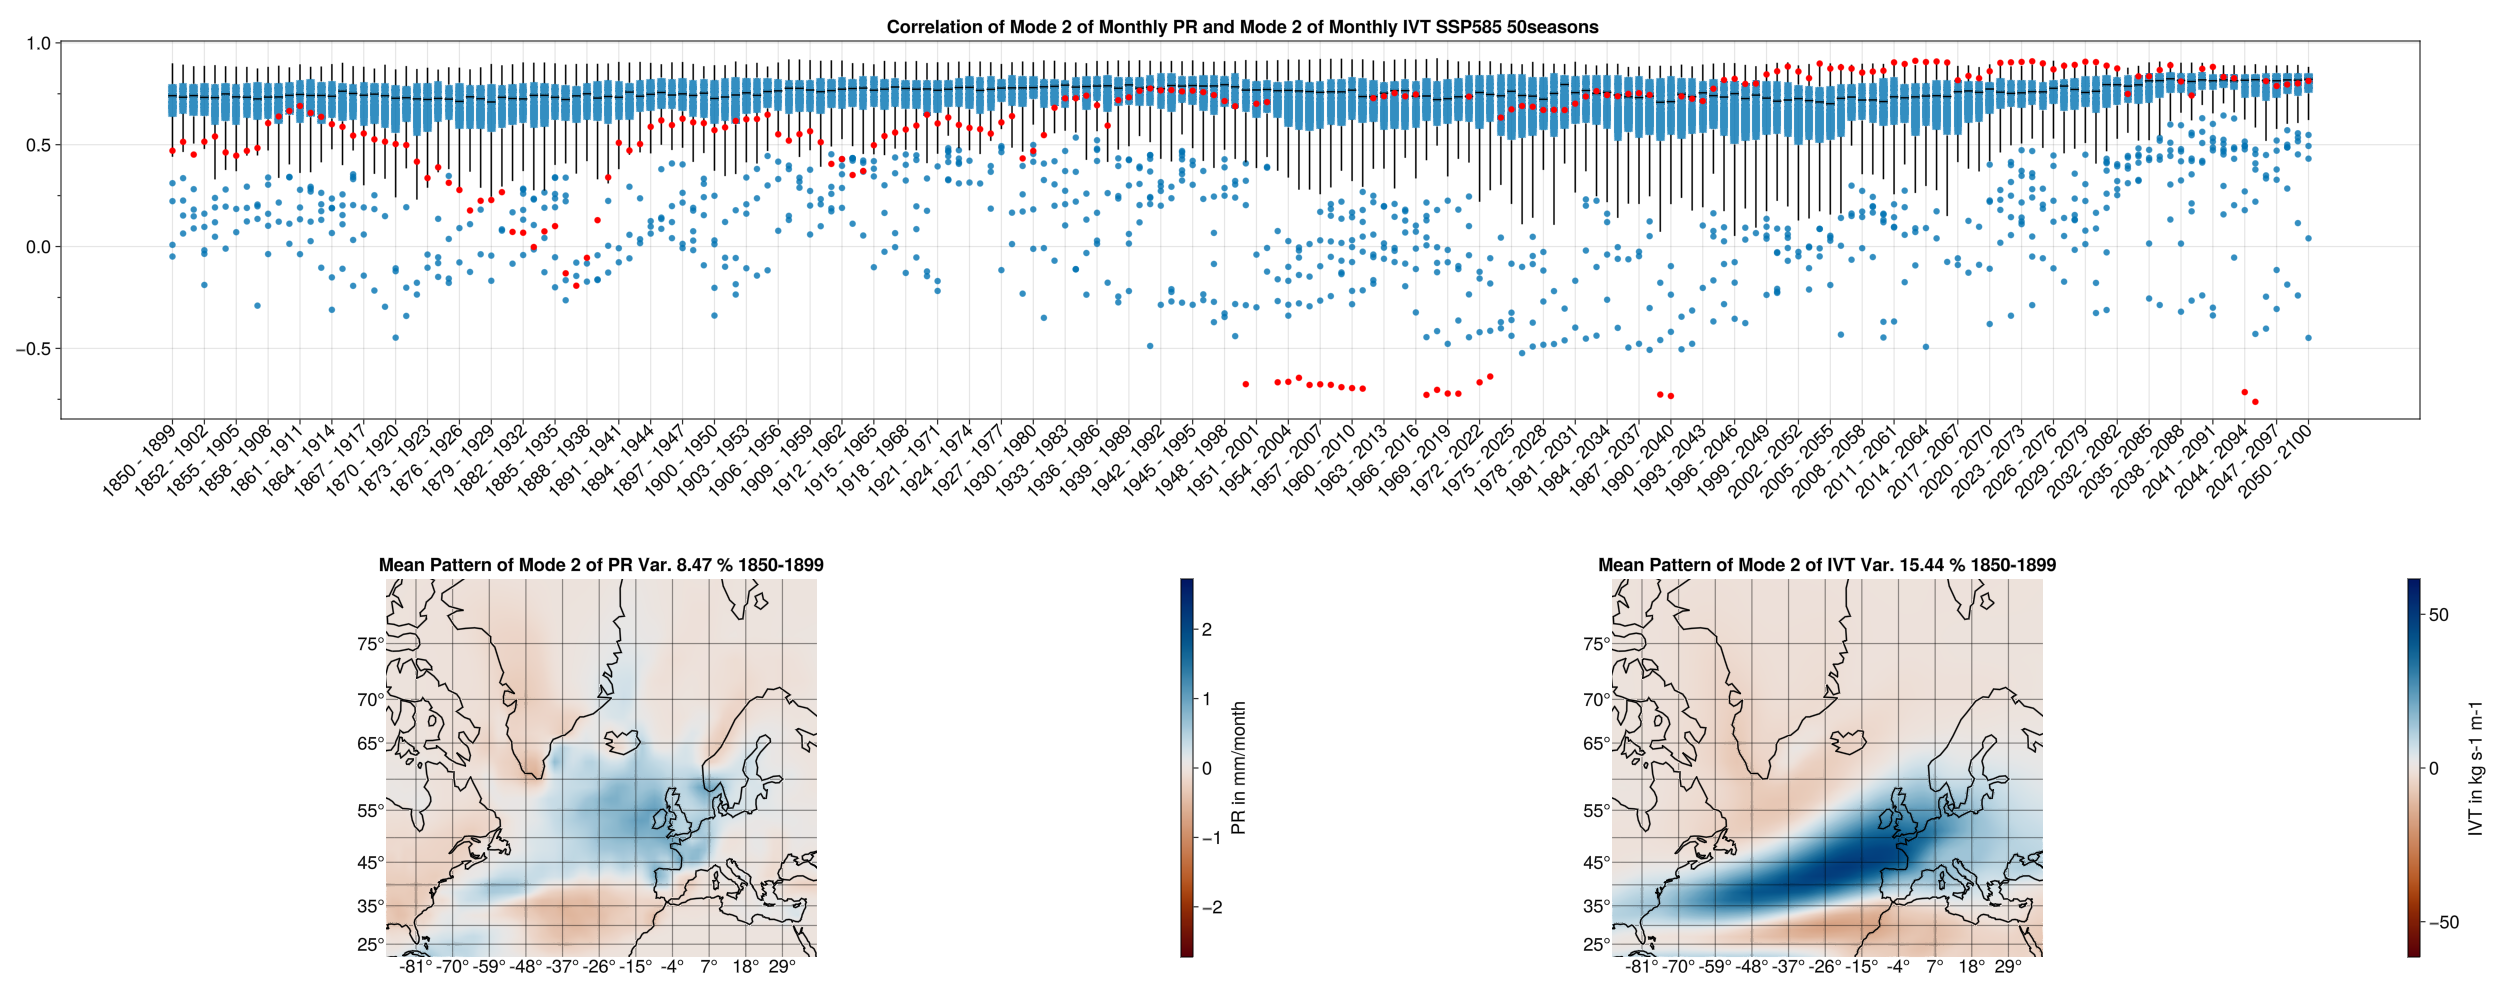
\includegraphics[width=\textwidth]{figures/correlation_boxplot_pr_ivt_modes22_ssp585_50seasons.png}
    \caption{Mode 2 of IVT and Mode 2 of precipitation}
    \label{fig:cor pr ivt modes22}
  \end{subfigure}
  \caption{Same as Figures~\ref{fig:cor pr ivt modes11} and \ref{fig:cor ivt psl modes22}, but with precipitation instead of sea level pressure.}
\end{figure}


From Figure~\ref{fig:cor pr ivt modes11} it is obvious that the primary modes of IVT and precipitation are very closely related. 
It shows a PCC of about $0.9$, with very little variance ocross the members. 
Also, there is barely a difference between SSP126 and SSP585. 
The secondary modes of IVT and precipitation look quite different: 
Although Figure~\ref{fig:cor pr ivt modes22} shows a quite high median PCC of about $0.75$, there are a lot of outliers, reaching down to the same extent in the negative spectrum. 
Also the preindustrial control simulation shows this kind of beviour in the scopes beginning at 1949 to 1974 (with interruptions). 
The explaination for this is pretty simple: Since this mode is pretty unstable across different members (see previous section), the alignment to the pattern shown in Figure~\ref{fig:cor pr ivt modes22} did not work very well, which causes the pattern (and following this also the EOF coefficients) to flip, resulting in result on the other side of the correlation spectrum. 



\begin{figure}[!tbp]
  \begin{subfigure}[b]{0.49\textwidth}
    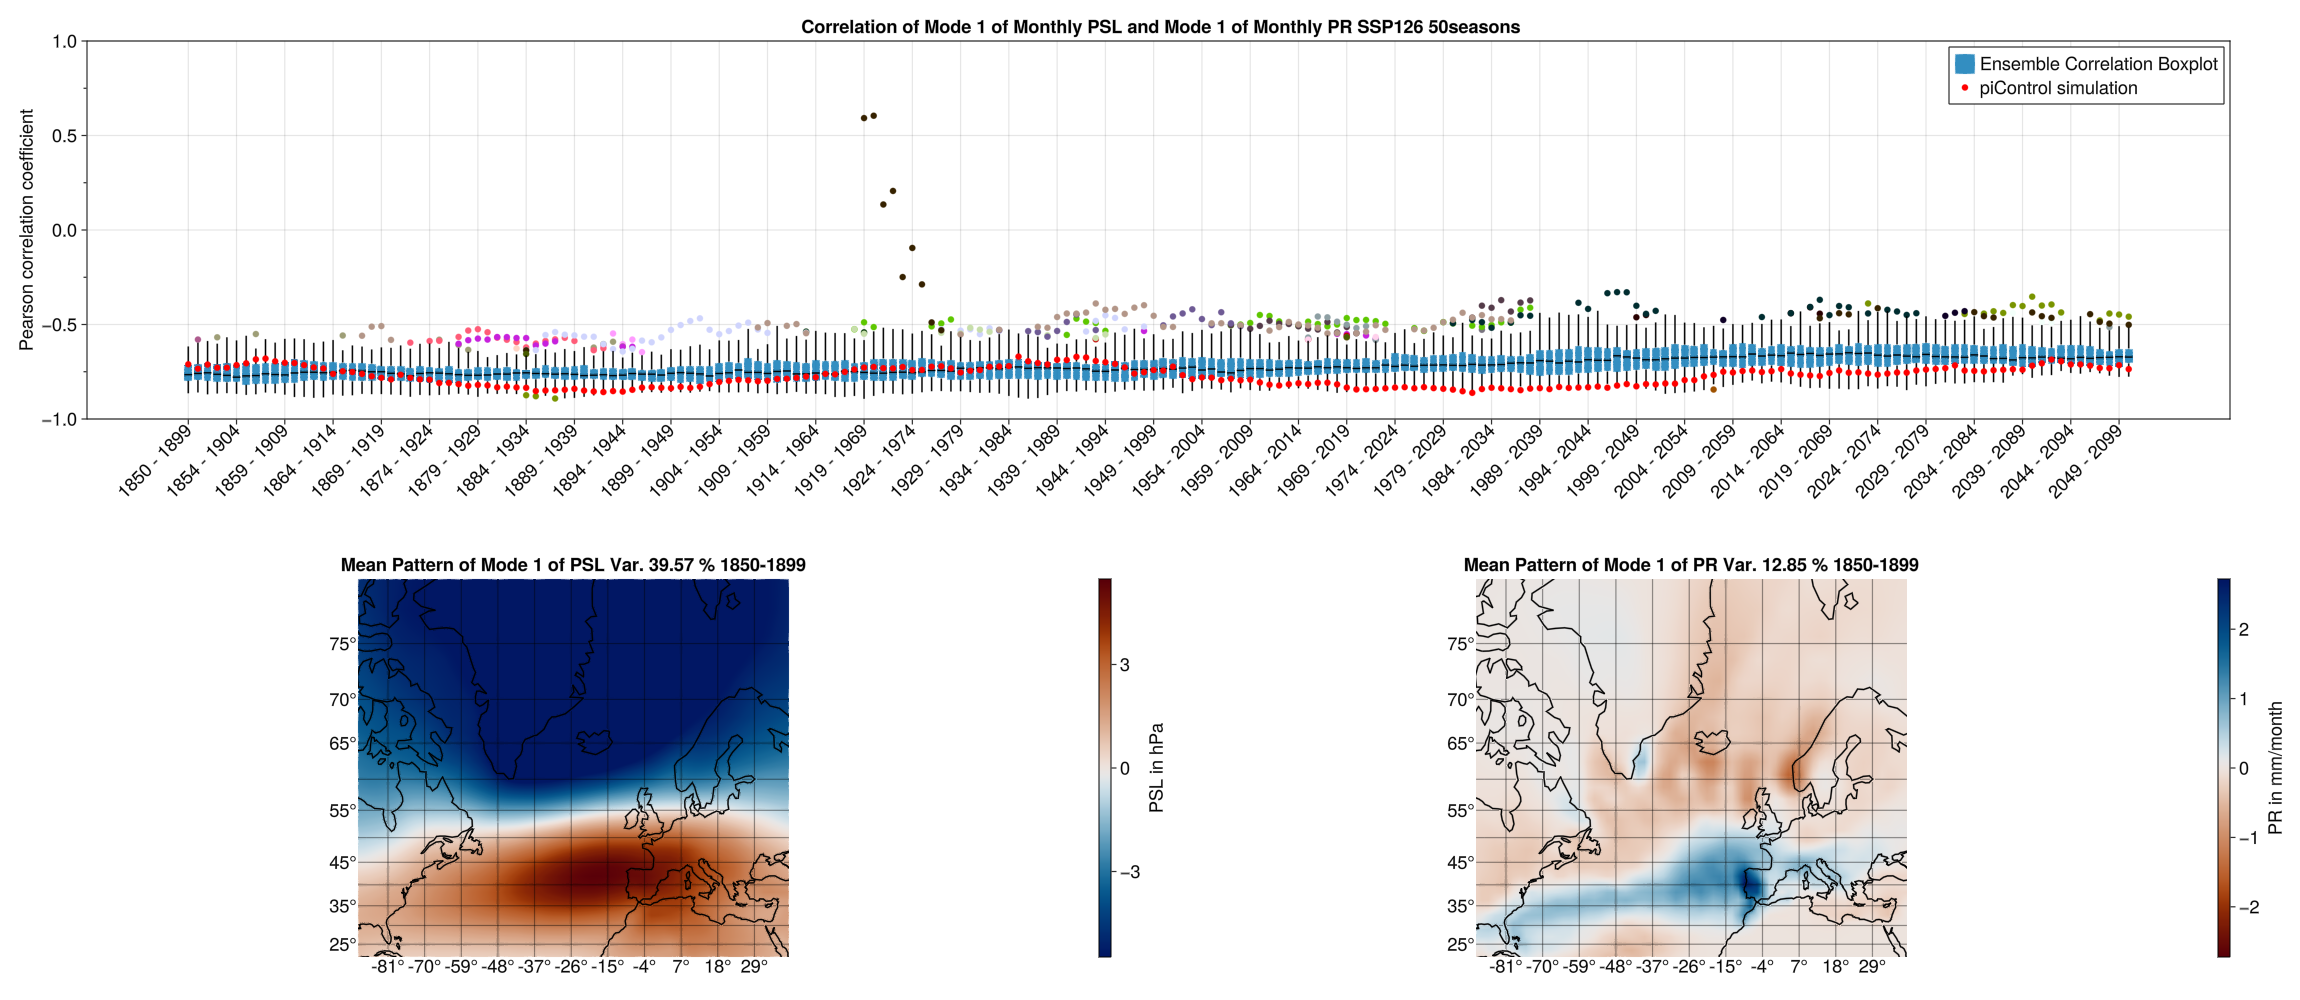
\includegraphics[width=\textwidth]{figures/correlation_boxplot_psl_pr_modes11_ssp126_50seasons.png}
    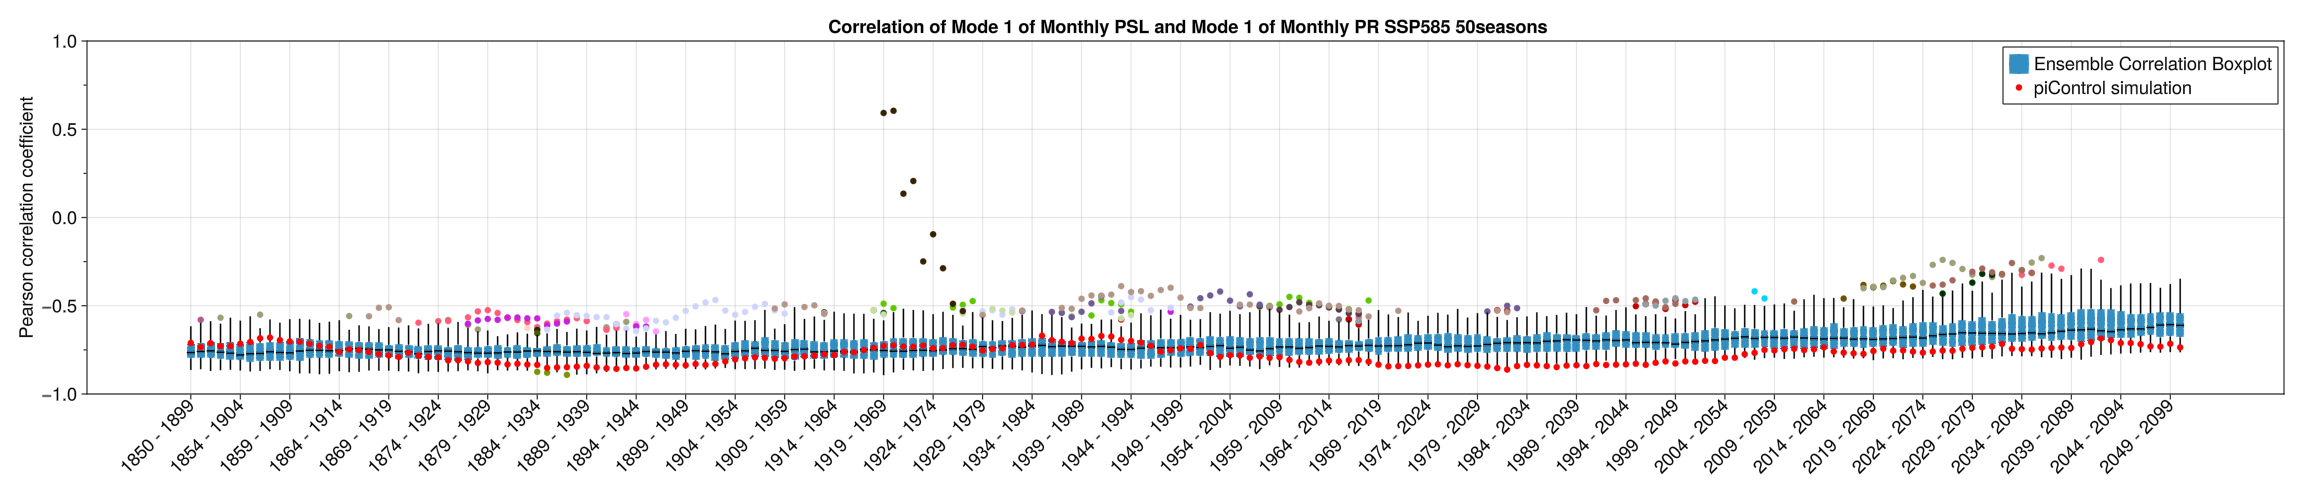
\includegraphics[width=\textwidth]{figures/correlation_boxplot_psl_pr_modes11_ssp585_50seasons.png}
    \caption{Mode 1 of IVT and Mode 1 of precipitation}
    \label{fig:cor psl pr modes11}
  \end{subfigure}
  \hfill
  \begin{subfigure}[b]{0.49\textwidth}
    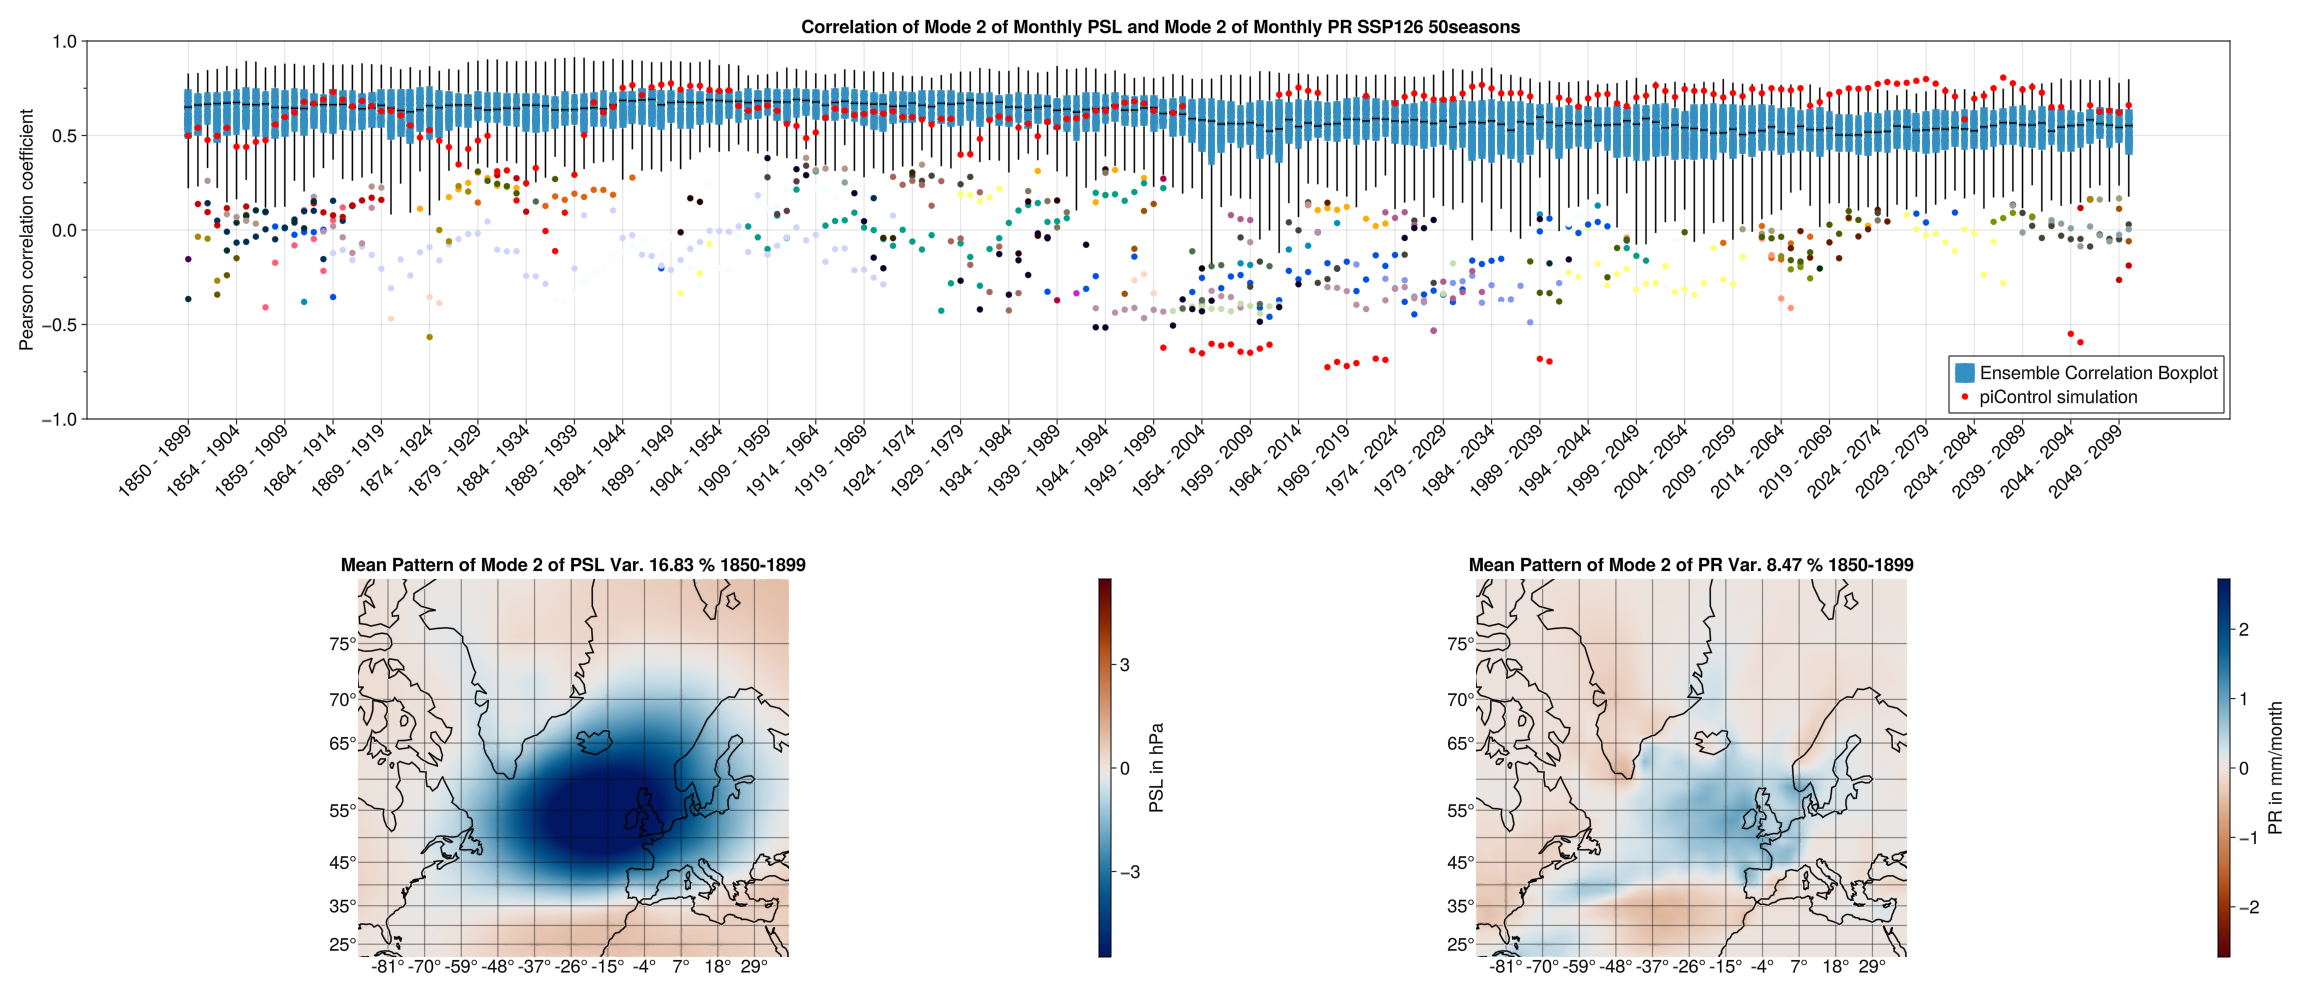
\includegraphics[width=\textwidth]{figures/correlation_boxplot_psl_pr_modes22_ssp126_50seasons.png}
    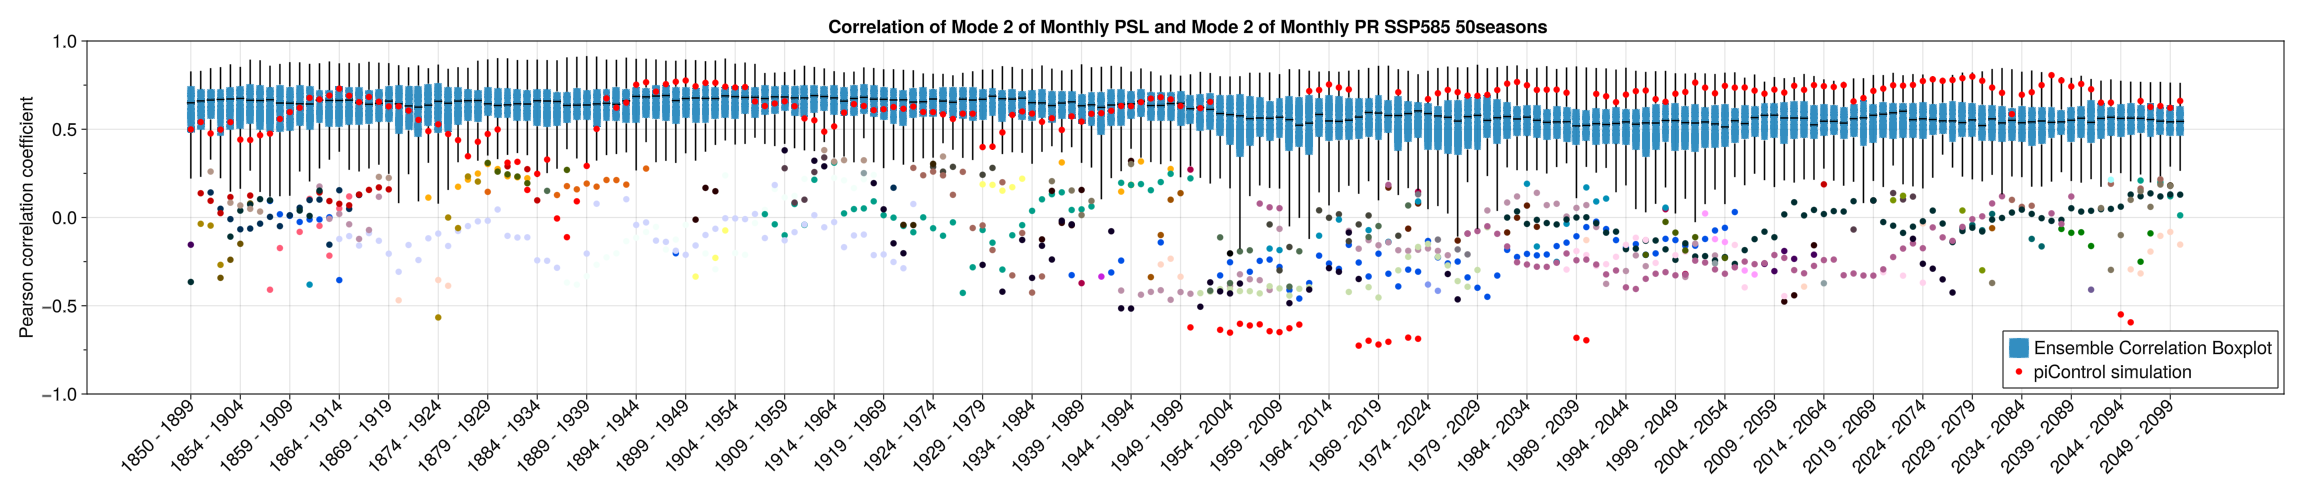
\includegraphics[width=\textwidth]{figures/correlation_boxplot_psl_pr_modes22_ssp585_50seasons.png}
    \caption{Mode 2 of IVT and Mode 2 of precipitation}
    \label{fig:cor psl pr modes22}
  \end{subfigure}
  \caption{Same as Figures~\ref{fig:cor pr ivt modes11} and \ref{fig:cor ivt psl modes22}, but with precipitation instead of sea level pressure.}
\end{figure}

Since the correlation between IVT and NAO/EAP and precipitation and IVT are already known, the analysis of their temporal correlation yields no surprises. 
Nevertheless, Figures~\ref{fig:cor psl pr modes11} and \ref{fig:cor psl pr modes22} show their evolution of correlation, showing the expected high negative ($\approx -0.75$) with the NAO index and the expected high positive correlation with the EAP index. 
Interestingly, the drop of correlation which was visible in Figure~\ref{fig:cor ivt psl modes22} does not appear in the relationship of precipitation and the EAP. 
But this could also be due to the amount of outliers (caused by incoherent, misaligned patterns of precipitation EOF2) warping the results. 




\subsection{Relationships of EOFs with Variables}

While the relationships of different patterns are interesting, EOFs are notoriously hard to interpret \cite{hannachi_empirical_2007, dommenget_cautionary_2002}. 
For the sea level pressure EOFs this has been solved, since the NAO and EAP (and there indices) are established physical modes and were first discovered using traditional measurements and evaluation of weather stations. 
It was then discovered that the EOFs of said fields also expose these patterns, and therefore useful to compute and represent these physical modes.  
Such an analysis does not yet exist for IVT and precipitation in Europe. 
Since the causality is quite clear (pressure oscillations influence the wind and therefore IVT and IVT influences precipitation), these directions of EOF mode $\rightarrow$ data correlation are explored. 
The most interesting of such analyses are the relationship between IVT EOF modes and precipitation data, since this could help to explain what influence certain modes have on the precipitation in Europe. 
Also depicted are the correlations between sea level pressure EOF modes and IVT data, to see the relationship between them. 


\begin{figure}[!htb]
  \begin{subfigure}[b]{0.32\textwidth}
    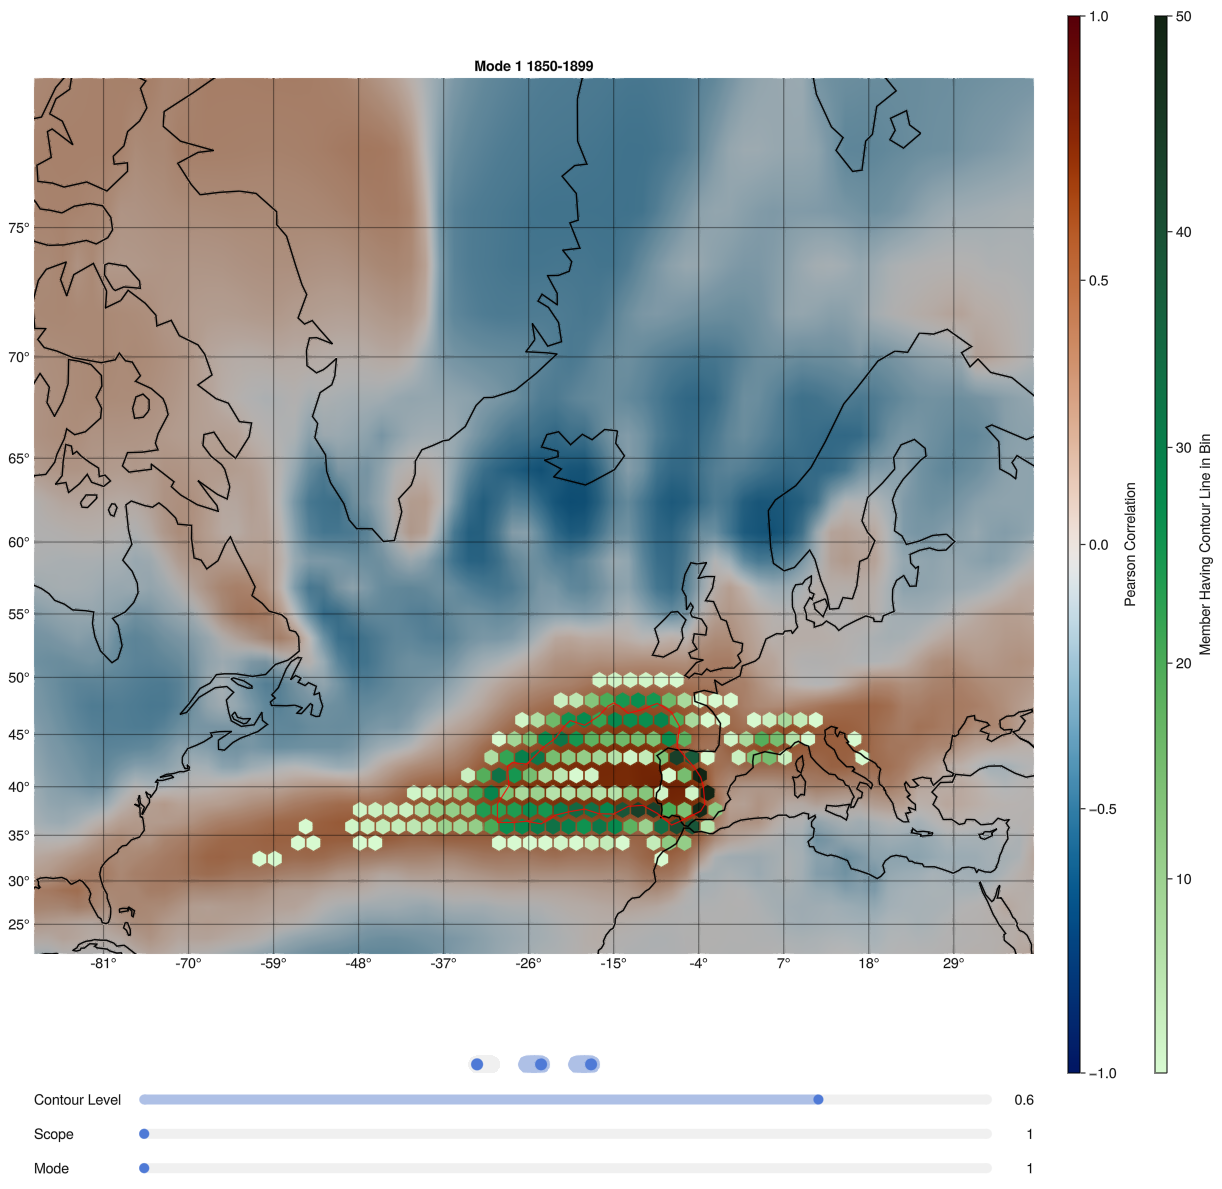
\includegraphics[width=\textwidth]{figures/ivt_pr_cor_mode1_historical_hexbin.png}
    \caption{Begin of historical simulation}
    \label{fig:ivt eof pr cor historical mode1}
  \end{subfigure}
  \hfill
  \begin{subfigure}[b]{0.32\textwidth}
    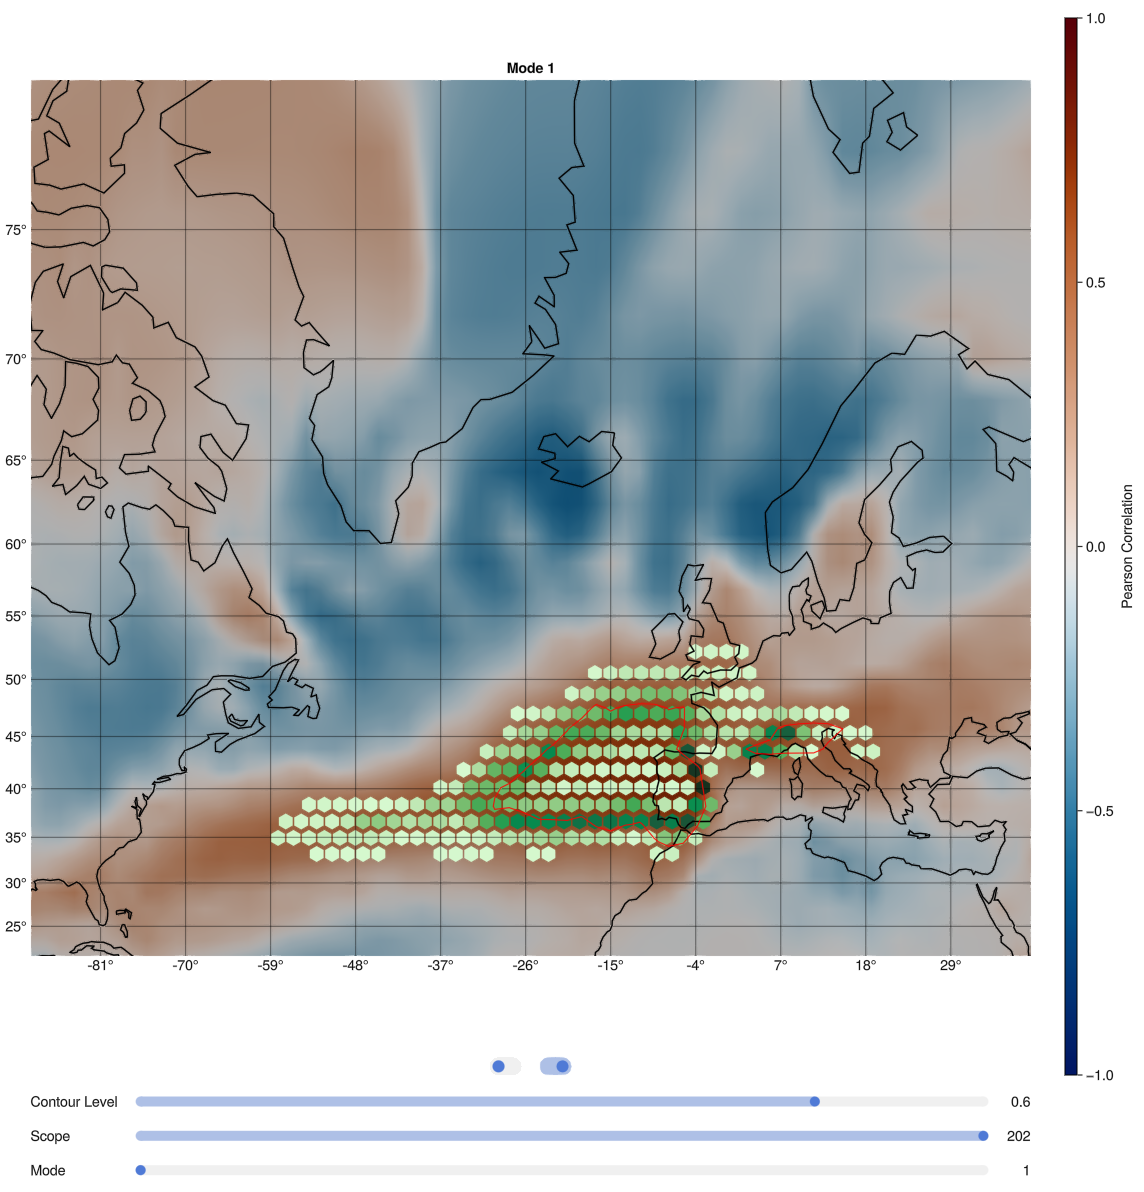
\includegraphics[width=\textwidth]{figures/ivt_pr_cor_mode1_ssp126_hexbin.png}
    \caption{End of SSP126} 
    \label{fig:ivt eof pr cor ssp126 mode1}
  \end{subfigure}
  \begin{subfigure}[b]{0.32\textwidth}
    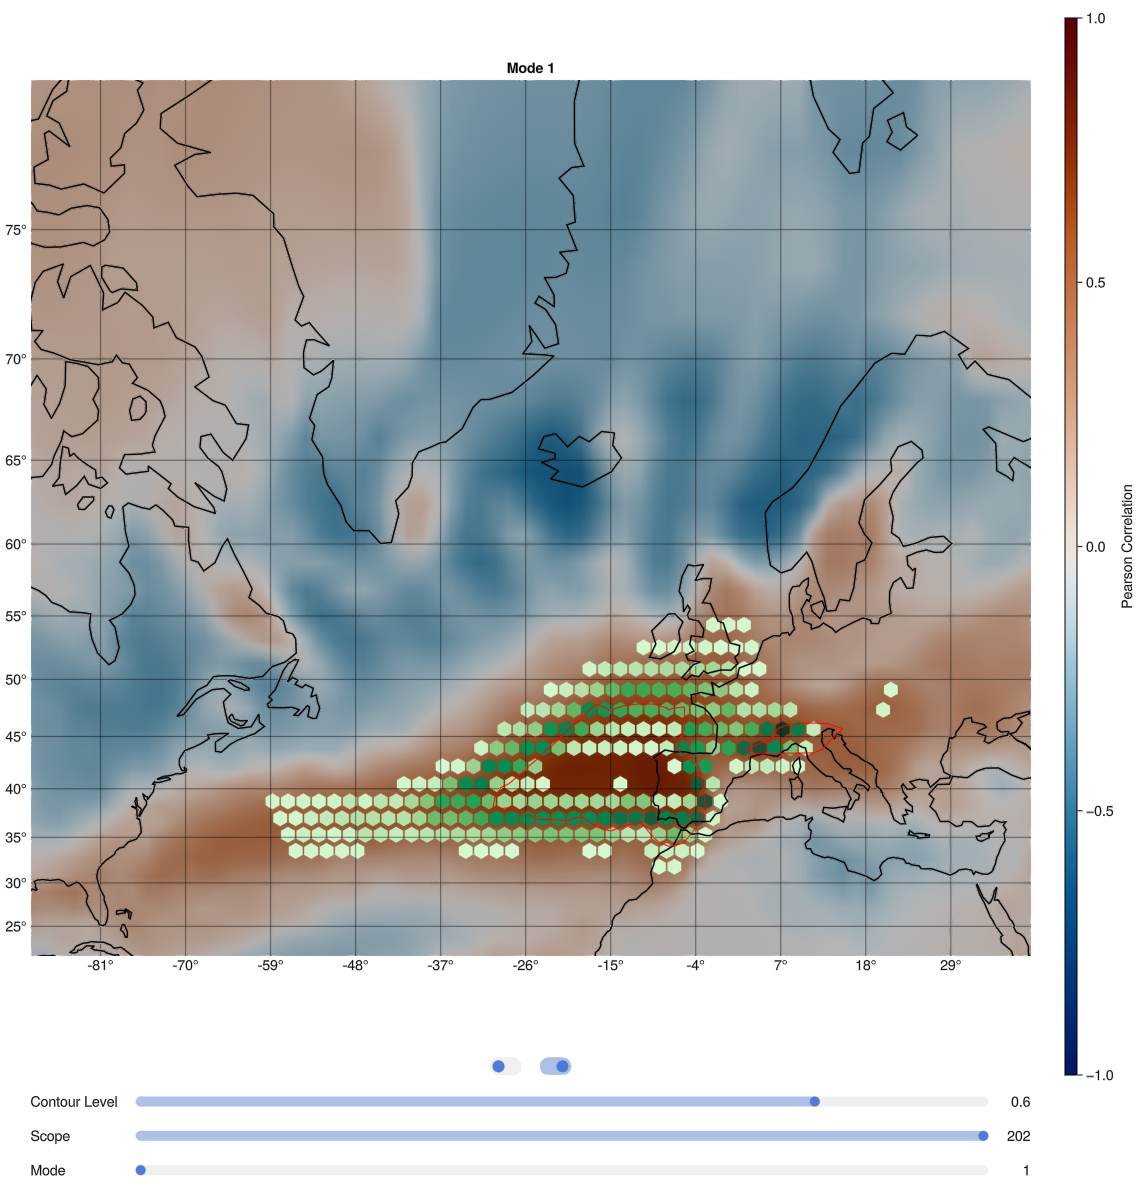
\includegraphics[width=\textwidth]{figures/ivt_pr_cor_mode1_ssp585_hexbin.png}
    \caption{End of SSP585}
    \label{fig:ivt eof pr cor ssp585 mode1}
  \end{subfigure}
  \caption{Correlation maps of IVT EOF mode 1 and precipitation data of the same scope. Hexbins show the probability of contour lines of $0.6$ passing through. The red line indicates the same contour line, but for the preindustrial control simulation.}
  \label{fig:ivt eof pr cor mode1}
\end{figure}


Figure~\ref{fig:ivt eof pr cor mode1} shows said correlation maps of mode 1 of the beginning of the historical simulation, the end of the SSP126 scenario, and the end of SSP585. 
The isocontours indicate the areas with PCC values higher than $0.6$, so areas where the actual precipitation behaves quite similarly to the dominant IVT pattern. 
This area is mainly the west coast of the Iberian Peninsula (area of highest correlation), the ocean westwards of it, and for some members, the Côte d'Azur. 
Looking at the evolution in time one can see that the area of high correlation do not change that much in SSP126. 
It seems to stretch a bit further north and more confident in the peak at the Côte d'Azur (darker green of hexbins in that area). 
Additionally, the Atlantic coast of France seems to be associated with PCC values $>0.6$ in some outliers of the ensemble. 
SSP585 shows the same changes, but far more pronounced: The outliers even reach the British Islands in the north, and the west coast of France seems to be part of the higher correlation area for most members, similar to the Côte d'Azur.
% But after all the contour of the piControl run (red), which changed only marginally, is still in the most likely (dark green) area. 

\begin{figure}[!htb]
  \begin{subfigure}[b]{0.32\textwidth}
    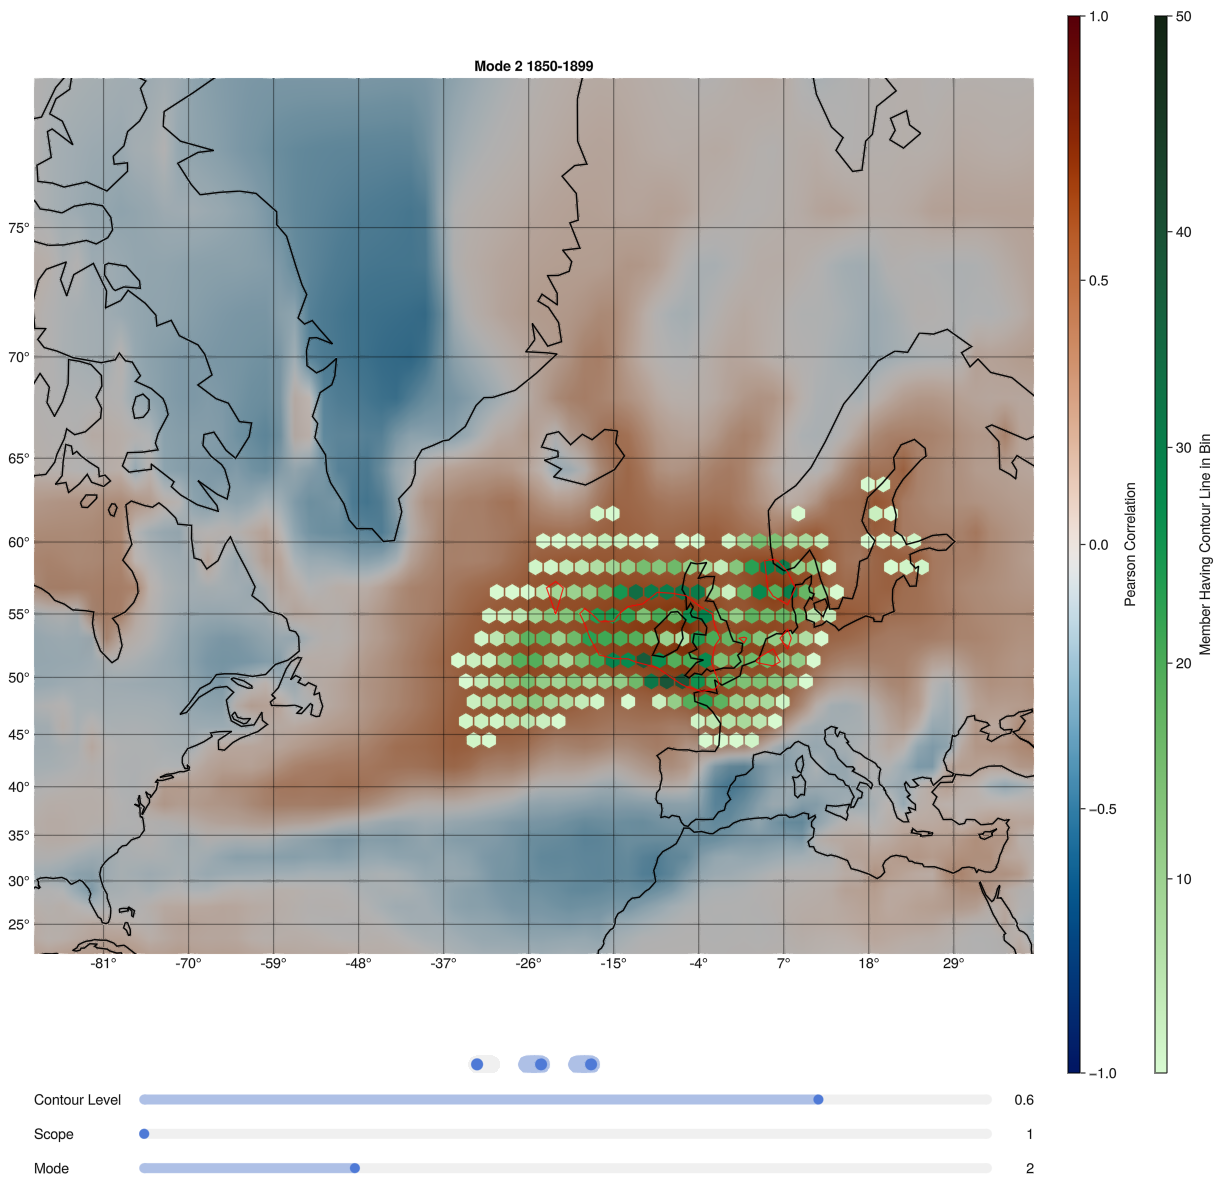
\includegraphics[width=\textwidth]{figures/ivt_pr_cor_mode2_historical_hexbin.png}
    \caption{Begin of historical simulation}
    \label{fig:ivt eof pr cor historical mode2}
  \end{subfigure}
  \hfill
  \begin{subfigure}[b]{0.32\textwidth}
    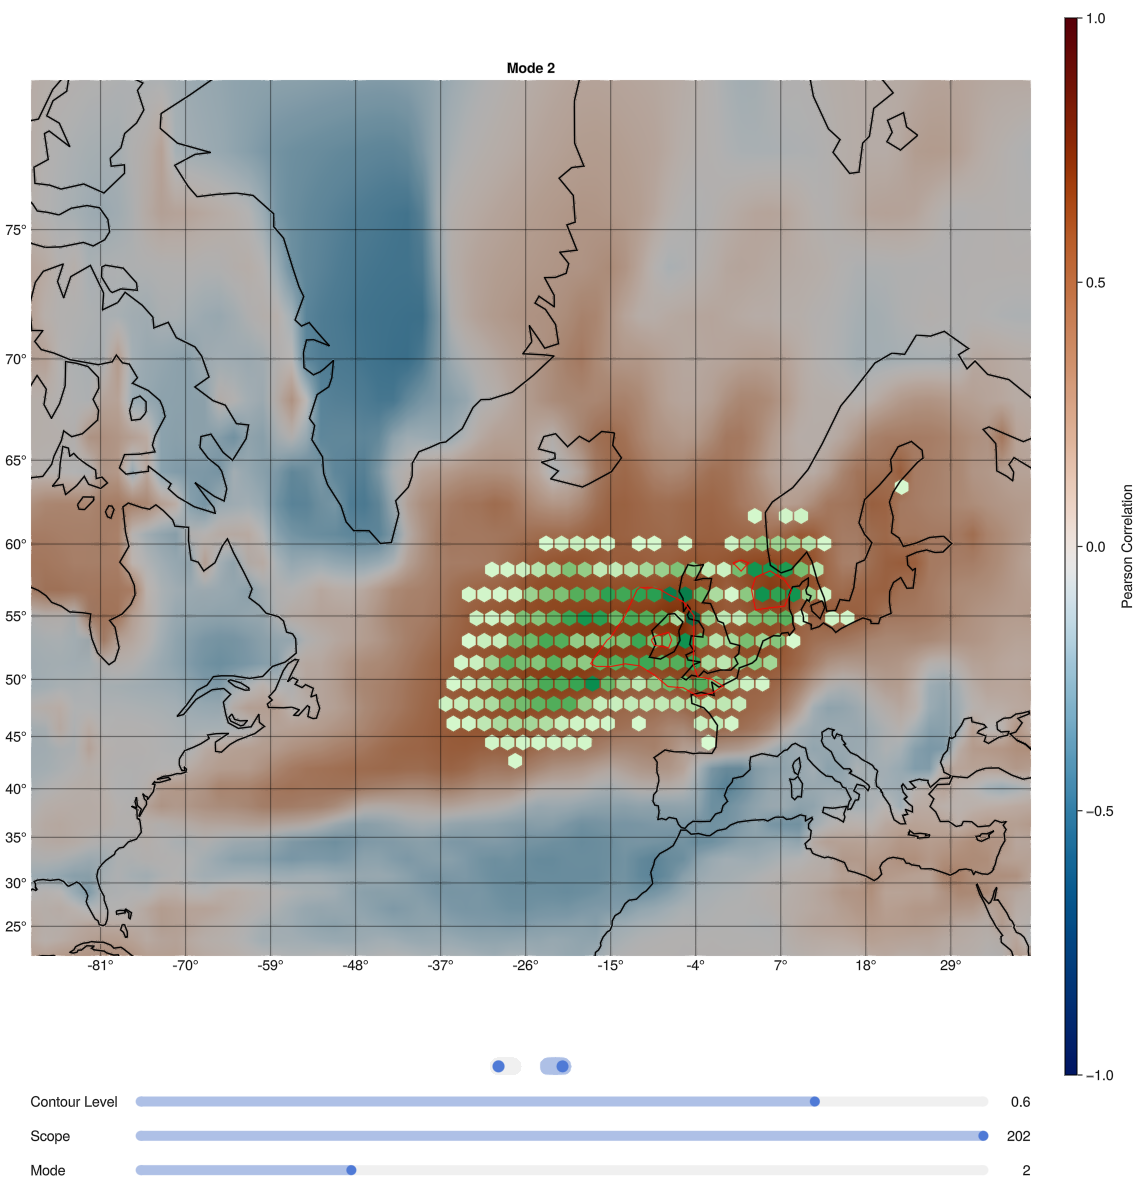
\includegraphics[width=\textwidth]{figures/ivt_pr_cor_mode2_ssp126_hexbin.png}
    \caption{End of SSP126} 
    \label{fig:ivt eof pr cor ssp126 mode2}
  \end{subfigure}
  \begin{subfigure}[b]{0.32\textwidth}
    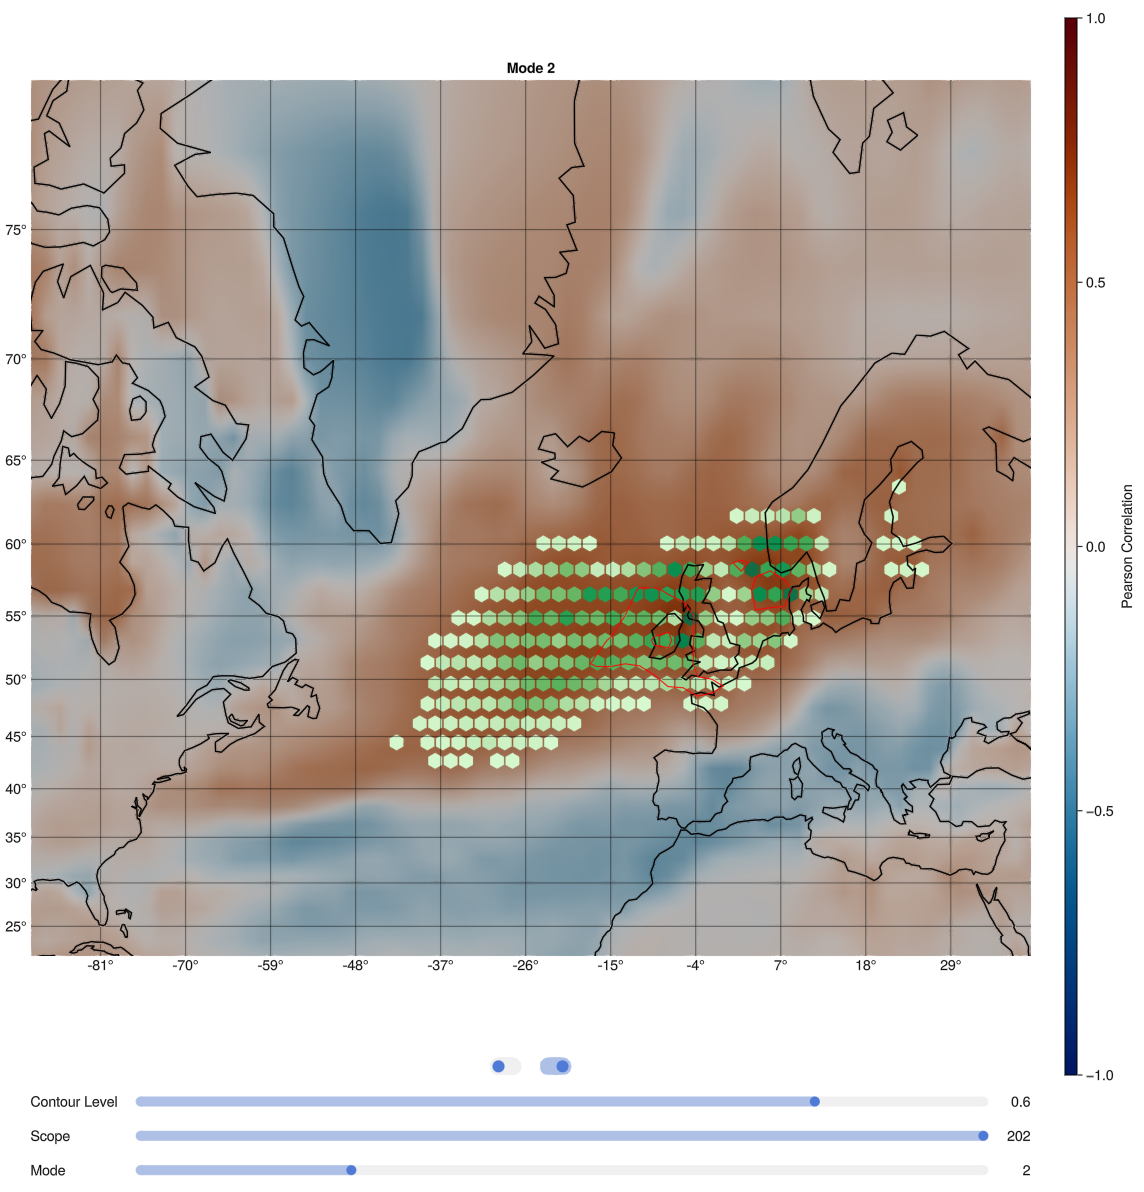
\includegraphics[width=\textwidth]{figures/ivt_pr_cor_mode2_ssp585_hexbin.png}
    \caption{End of SSP585}
    \label{fig:ivt eof pr cor ssp585 mode2}
  \end{subfigure}
  \caption{Same as Figures~\ref{fig:ivt eof pr cor mode1} but with mode 2 of IVT EOF.}
  \label{fig:ivt eof pr cor mode2}
\end{figure}

Figure~\ref{fig:ivt eof pr cor mode2} shows the same analysis, but for mode 2 of IVT EOF. 
The area of higher (positive) correlation are here especially the west coasts of the British Islands and Scandinavia, but also the ocean westwards of them, the whole west coast of Europe, the North Sea. 
Also, there are only a few members indicating that correlation level in the Gulf of Bothnia (between Finland and Sweden), but these seem to be outliers. 
The end of the SSP126 scenario looks quite similar to the beginning of the historical simulation, except that the contour lines seem to reach less into European Mainland, and are less confident on the west coast of France.  
This could be due to the increased influence of IVT EOF mode one in the same area, which reduces the effect of the secondary mode on that coast. 


\begin{figure}[!htb]
  \begin{subfigure}[b]{0.32\textwidth}
    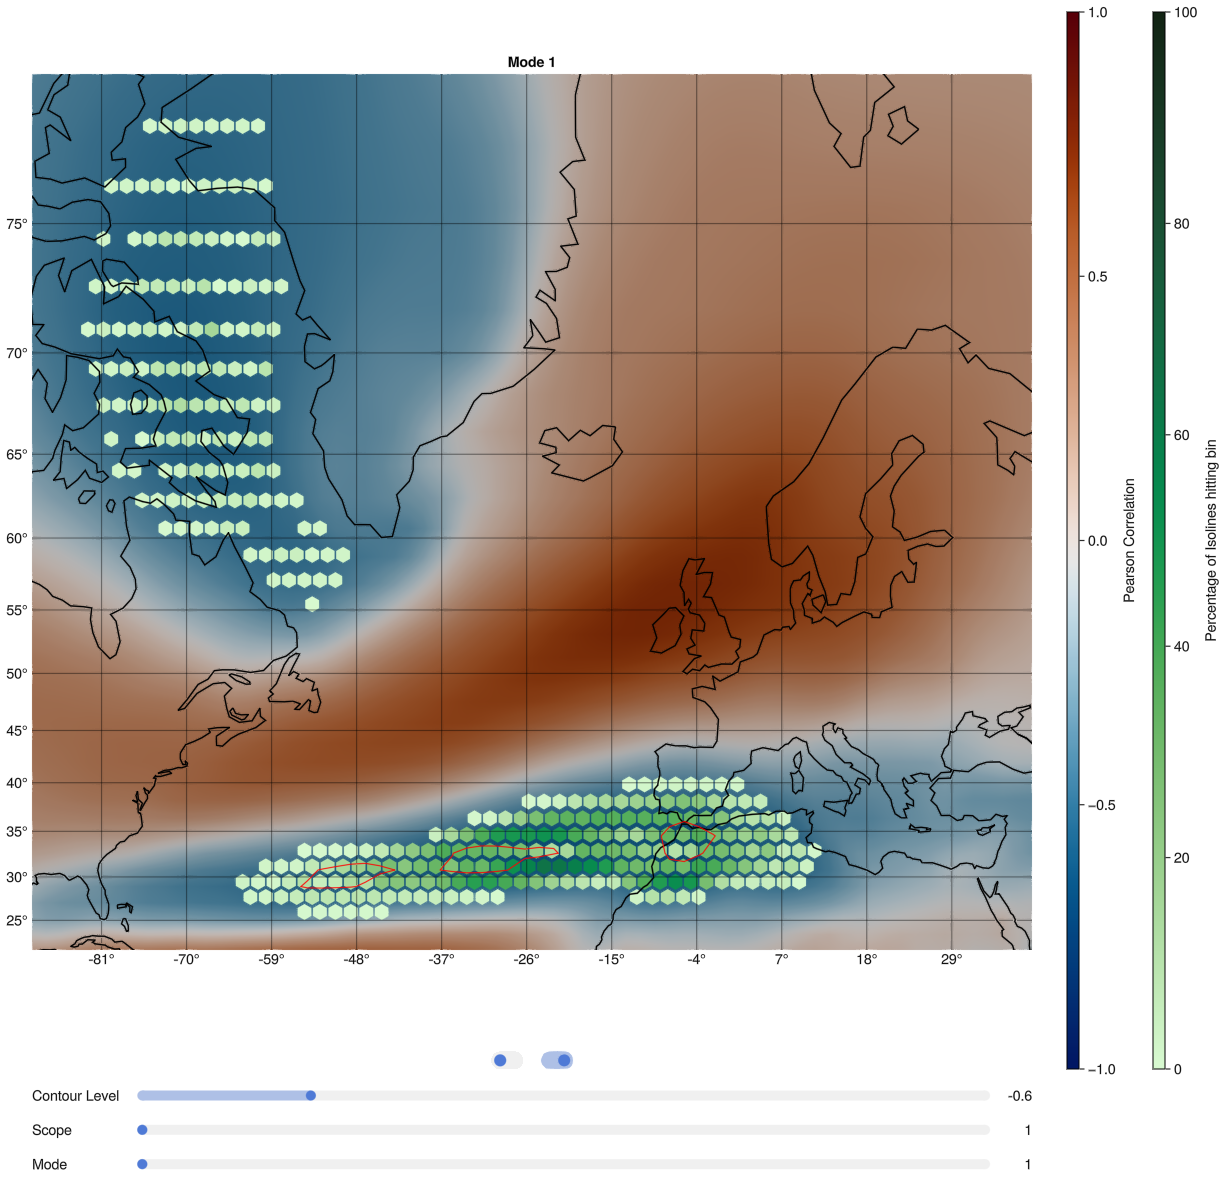
\includegraphics[width=\textwidth]{figures/psl_ivt_cor_mode1_historical.png}
    \caption{Begin of historical simulation}
    \label{fig:psl eof ivt cor historical mode1}
  \end{subfigure}
  \hfill
  \begin{subfigure}[b]{0.32\textwidth}
    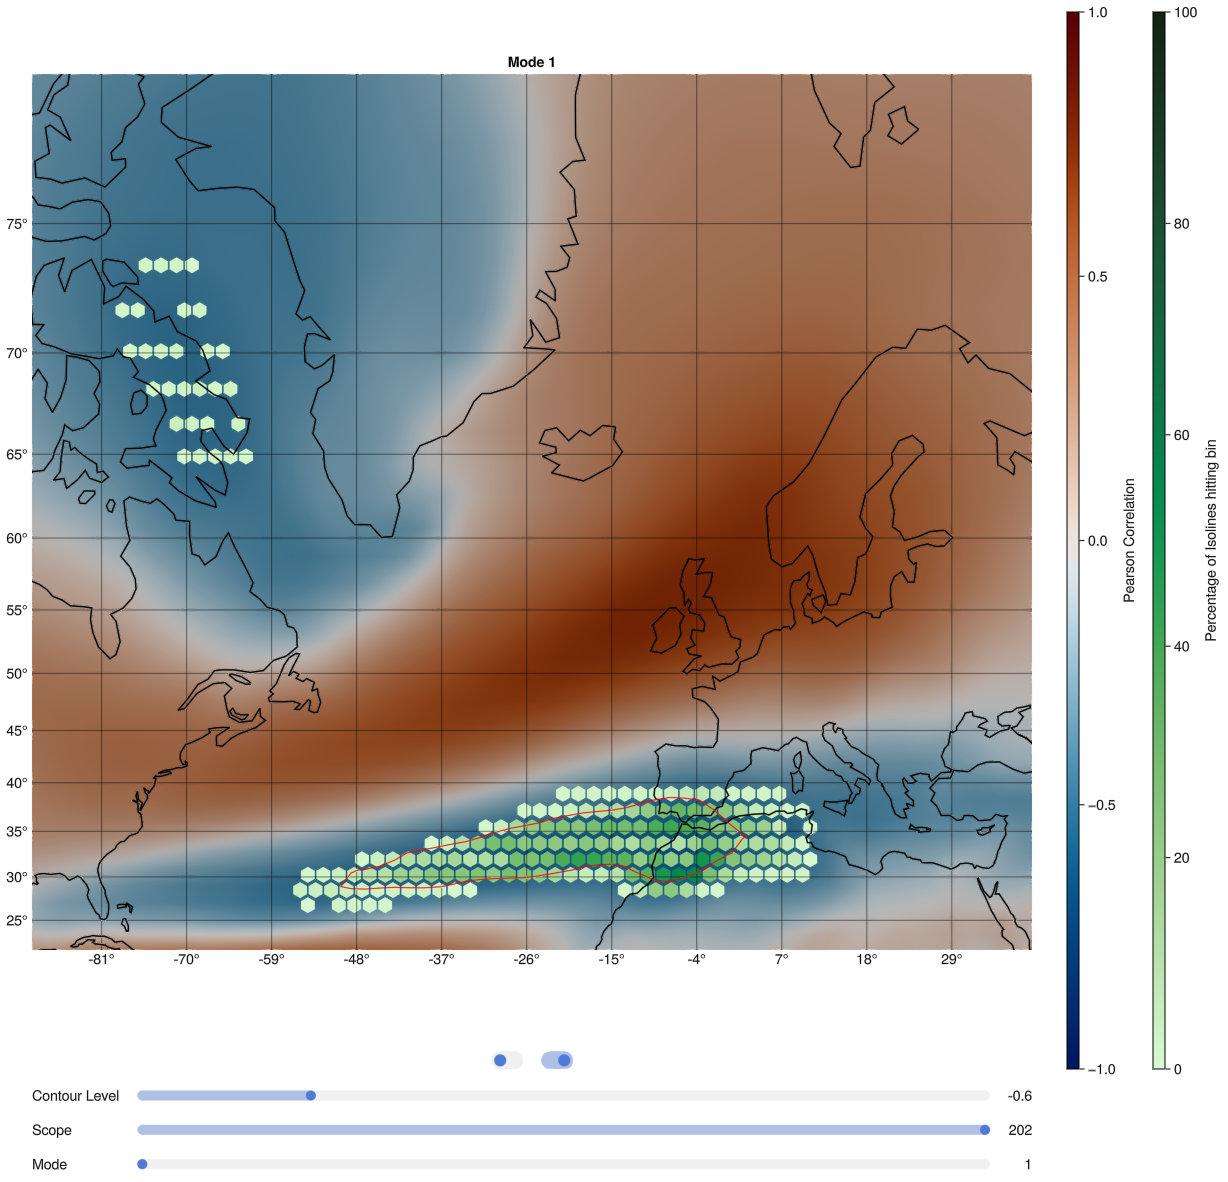
\includegraphics[width=\textwidth]{figures/psl_ivt_cor_mode1_ssp126.png}
    \caption{End of SSP126} 
    \label{fig:psl eof ivt cor ssp126 mode1}
  \end{subfigure}
  \begin{subfigure}[b]{0.32\textwidth}
    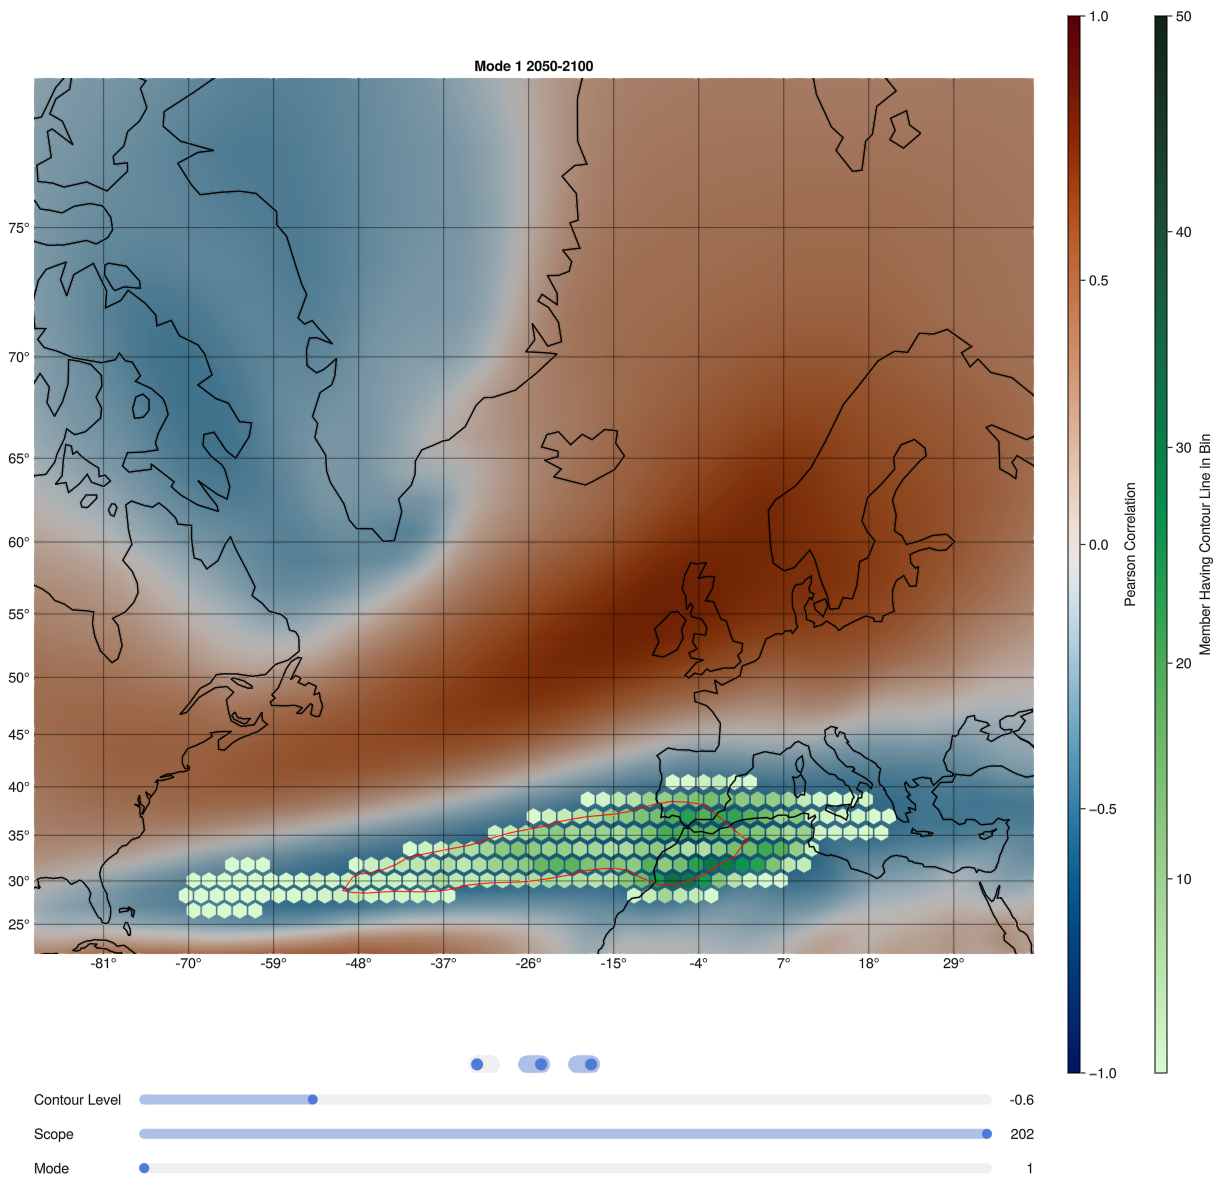
\includegraphics[width=\textwidth]{figures/psl_ivt_cor_mode1_ssp585.png}
    \caption{End of SSP585}
    \label{fig:psl eof ivt cor ssp585 mode1}
  \end{subfigure}
  \caption{Same as Figure~\ref{fig:ivt eof pr cor mode1}, but with sea level pressure mode (NAO index) and IVT data correlation. Also, hexbins indicate the contour lines of $-0.6$ PCC.}
  \label{fig:psl eof ivt cor mode1}
\end{figure}


Figure~\ref{fig:psl eof ivt cor mode1} shows the same correlation maps, but with the primary PSL EOF (the NAO index) and IVT data. 
This has the goal of seeing how the oscillation indices are connected to the actual IVT data, and maybe even track a northward shift there. 
In the first mode the negative correlations below $-0.6$ are shown, which should display the areas assiciated with the inverse of the normal NAO (pressure low in the south and pressure high in the north). 
In general, the hexbins are not as dark green as in the previous figures, indicating that the members do not agree as unanimous. 
The highest are of correlation on that level is on the west coast of the Iberian Peninsula and Morocco, and the ocean westwards of that are. 
In the historical simulation, also the Labrador Sea features a few light green hexbins, indicating that only a few members seem to have that kind of correlation between IVT and the NAO index. 
The change between the beginning of the historical simulation and the ends of SSP126 and SSP585 are only marginal, no (northward or whatsoever) shift of the really important dark green hexbins. 
This means that only a few outliers of the members changed, the contour lines of the largest quantity of members stays pretty much the same. 


\begin{figure}[!htb]
  \begin{subfigure}[b]{0.32\textwidth}
    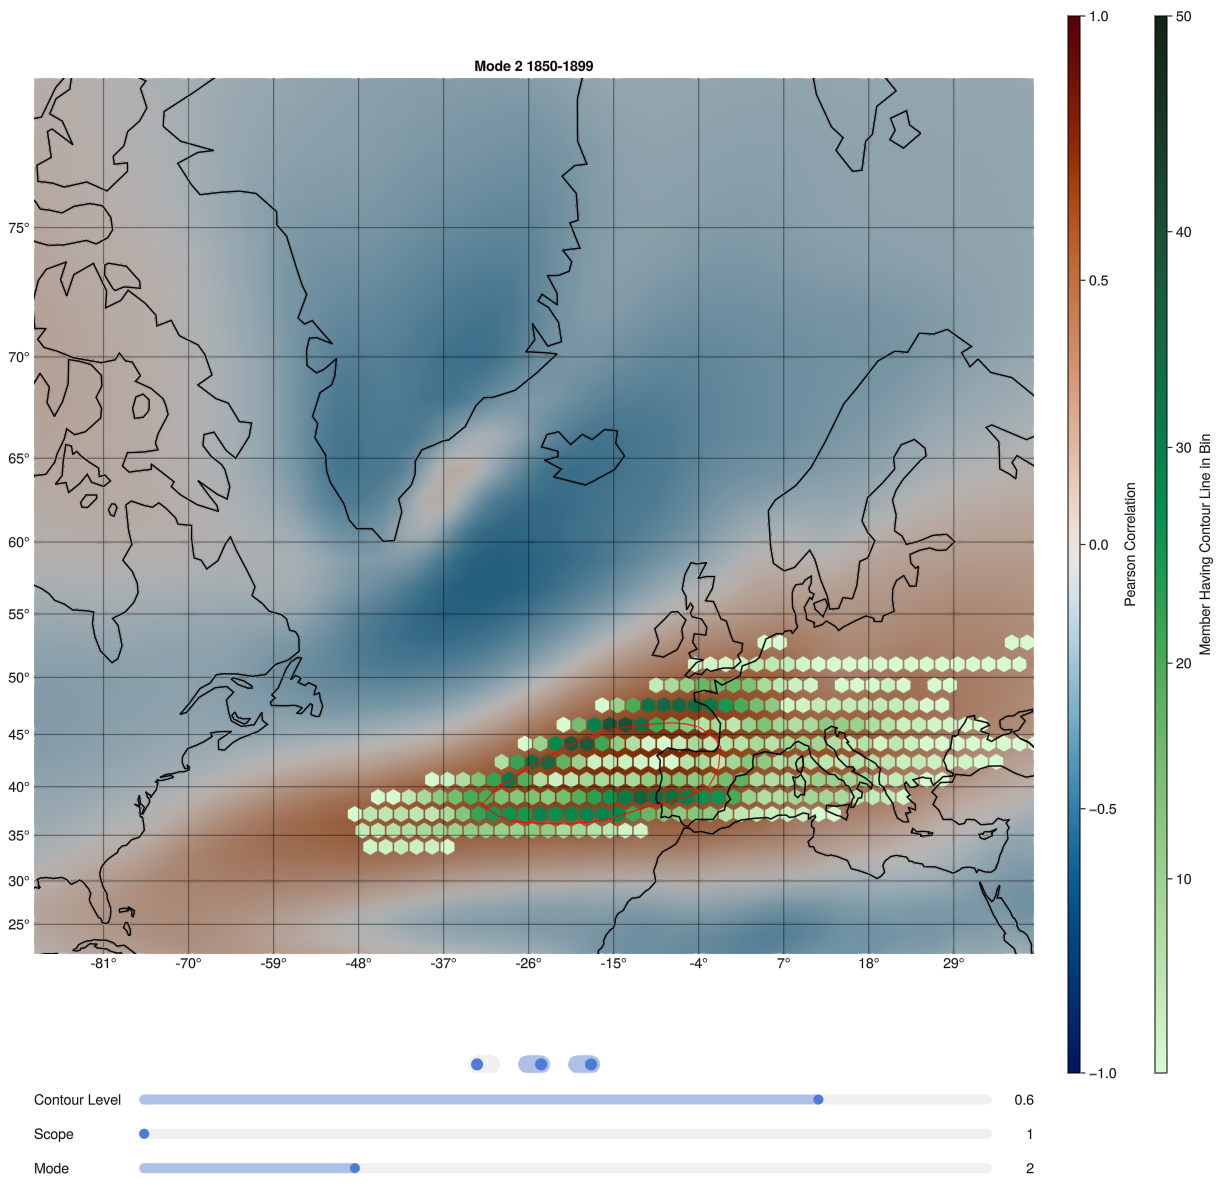
\includegraphics[width=\textwidth]{figures/psl_ivt_cor_mode2_historical.png}
    \caption{Begin of historical simulation}
    \label{fig:psl eof ivt cor historical mode2}
  \end{subfigure}
  \hfill
  \begin{subfigure}[b]{0.32\textwidth}
    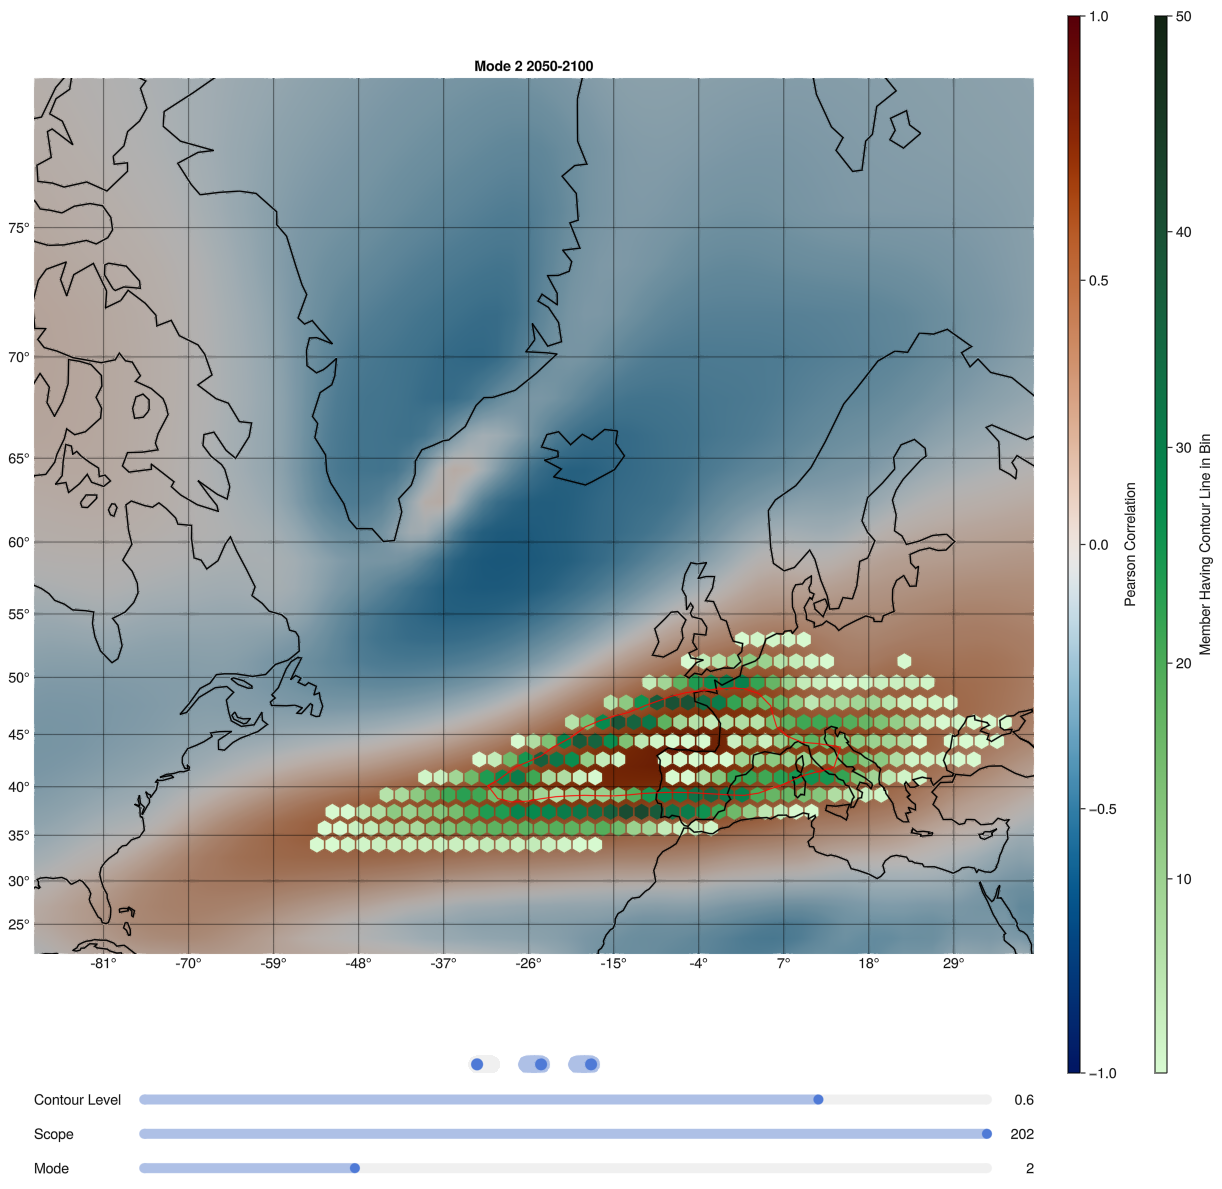
\includegraphics[width=\textwidth]{figures/psl_ivt_cor_mode2_ssp126.png}
    \caption{End of SSP126} 
    \label{fig:psl eof ivt cor ssp126 mode2}
  \end{subfigure}
  \begin{subfigure}[b]{0.32\textwidth}
    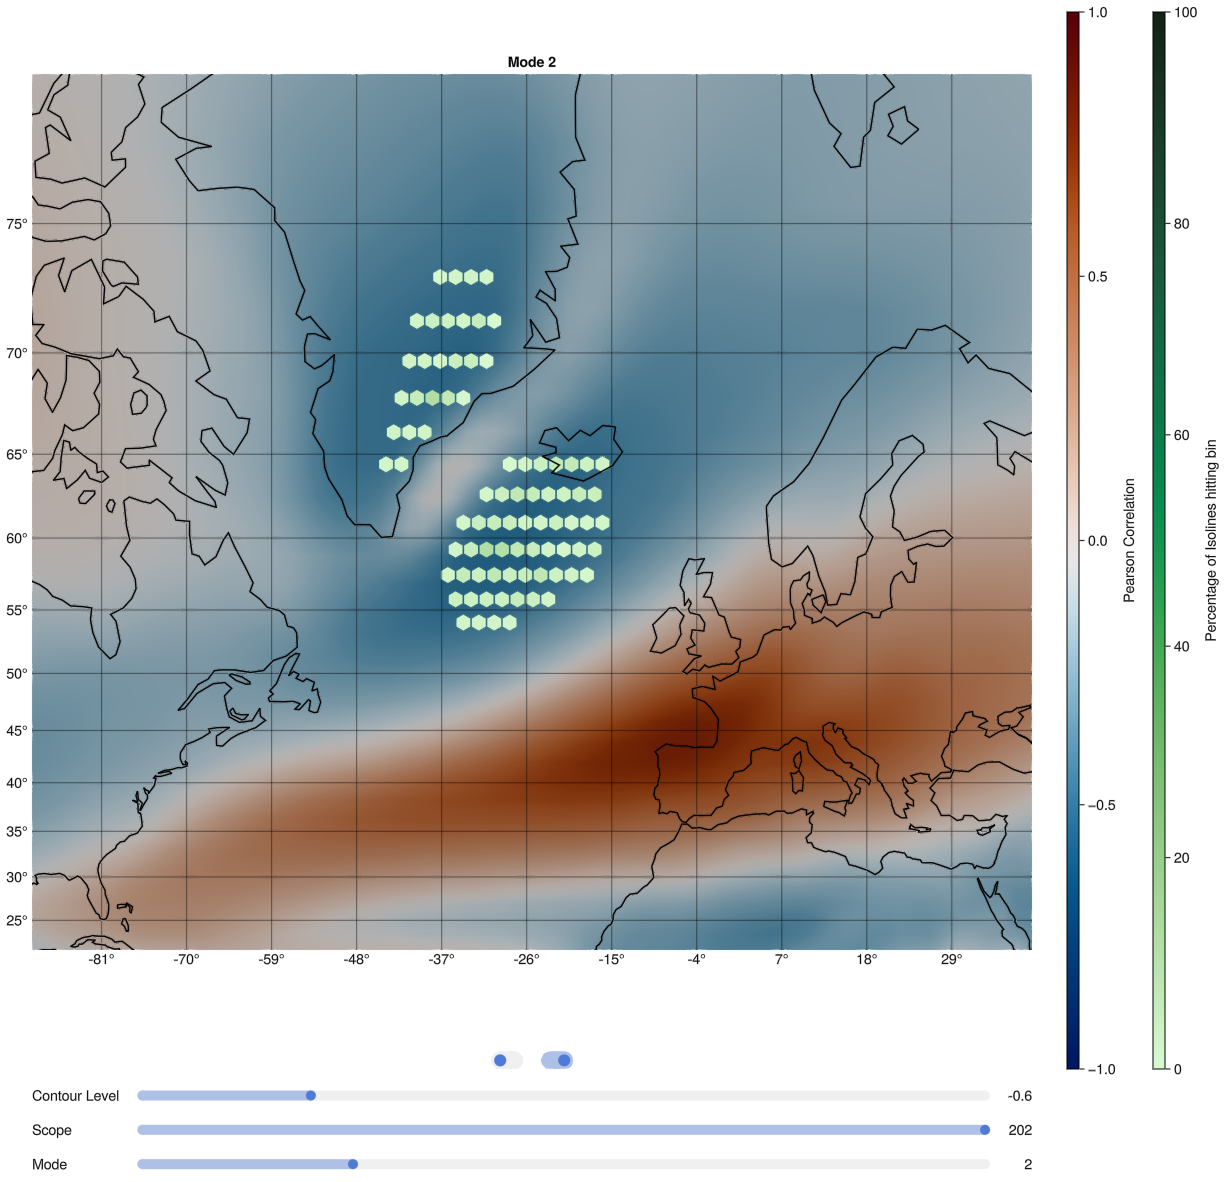
\includegraphics[width=\textwidth]{figures/psl_ivt_cor_mode2_ssp585.png}
    \caption{End of SSP585}
    \label{fig:psl eof ivt cor ssp585 mode2}
  \end{subfigure}
  \caption{Same as Figure~\ref{fig:psl eof ivt cor mode1}, but with the second PSL mode (EAP index).}
  \label{fig:psl eof ivt cor mode2}
\end{figure}

\todo{Replace with positive correlations since the correlations are also positive!}


\section{Discussion}
\label{sec:discussion}

This section discusses the results from the previous sections as well as the effectiveness of the introduced hexbin visualization. 

\subsection{Insights about the patterns}

First, the real interpretation of the results is not the topic of this Thesis, since it requires the knowledge of real domain experts (meteorologists or climate scientists). 
The focus of this work was a) the generation of EOF patterns of moisture related variables and b) the visualization of the variability across ensemble members. 
Nevertheless, the results still yield some interesting differences between the historical simulation and both evaluated future scenarios. 
While the benefits of analyzing EOFs instead of the original data are great, they are notoriously hard to interpret with regard to the actual atmospheric physics behind them \cite{dommenget_cautionary_2002, hannachi_empirical_2007}.
The reasons mostly named for this are the forced orthogonality of modes, which does not really exist in the real world \cite{hannachi_empirical_2007}, and the \enquote{hallucination} of modes, which means creating certain modes which have no equivalent in the real data/world (which was shown in detail in the work of \citeauthorwork{dommenget_cautionary_2002}). 
The reason for said hallucinations is also the forced orthogonality of EOF modes. 
Yet, the importance of the dominant modes of IVT were mentioned and analyzed in previous work \cite{salstein_modes_1983, zou_interdecadal_2018}. 
Therefor, this section tries to summarize the most important discoveries of the European, moisture related EOFs, their relationships, and their development in future scenarios. 

Starting with the analysis of the variance encoded by different modes (Section~\ref{sec:results encoded variance}), the most interesting discoveries are the changing importance of modes in different future scenarios. 
Most importantly are here the clearly visible increase in SSP585 of EOF2 of PSL (EAP) by $2-3 \%$ and EOF1 of precipitation data by a similar amount. 
This could be explained by the increased area covered by this mode in SSP585, shown in Section~\ref{sec:spatial pattern evolution}. 
By covering a larger area, this mode can cover a larger portion of the whole datasets anomaly. 
Also, this suggests that a larger area behaves more similar in time ($\equiv$ can be represented with the same temporal patterns/EOF coefficients). 


One of the most interesting results of this analysis is the very strong relationship of the primary modes of IVT and precipitation EOFs with a correlation coefficient of about $0.9$.
This may indicate that EOF1 of IVT is a driver of that particular precipitation mode, since water vapor transport causes precipitation (and not vice versa). 
The primary mode of PR seems to be especially important for the precipitation in the east (coast) of the Iberian Peninsula, which would then be also true for the primary EOF of IVT. 
This impression is also reinforced by looking at the correlation maps of IVT EOF1 and precipitation data (Figure~\ref{fig:ivt eof pr cor mode1}), which shows very high correlation values with the temporal pattern of said mode on the east coast of the Iberian Peninsula. 
The pronounced northward expansion of both PR EOF1 and the correlation between IVT EOF1 and precipitation could also be explained with the northward shift/expansion of the dominant IVT mode, which means this mode influences a larger region of Europe in heavier climate change. 

Also interesting is the change of the spatial component of the secondary IVT EOF. 
Mainly, because the consequences of that are not entirely clear. 
The correlation between IVT EOF2 and precipitation do show some changes in SSP585 (less influence on the west coast of Europe), but this could also be due to the increased influence of IVT EOF1. 
Additionally, the relationship with the EAP index (Figure~\ref{fig:cor ivt psl modes22}), seems to drop in the later years of the scenario, in difference to SSP126. 

The analysis of the standard deviation of the different modes had the goal of showing the fluctuations and the evolution thereof. 
Since the EOF coefficients have a SD of one in their normal (unscaled) state, it is entirely dependent on the scaling, encoded in the singular values of the respective mode. \todo{THink about this. is this true?} 
Most notably is here the striking difference between SSP126 and SSP585 in variance of the dominant IVT EOF modes. 
Since this is not reflected in the percentage share of variance in those modes, the most likely answer is that the variance of IVT increases in general more in SSP585.
A similar pattern can be seen in Figure~\ref{fig:std pr evolution}, but this can be explained with a combination of increased total variance and the increase of the percentage share of PR EOF1. 

\todo{Maybe add paragraph of unanswered questions}
In the end it needs to be stressed that these are just speculations, and the actual interpretation needs to be performed by domain experts. 

% \begin{itemize}
%   \item in general, real interpretation of the results require the knowledge of a domain expert
%   \item But: the analysis shows some changes during climate change, and some could be attributed to intensity thereof 
%   \item but still: some of the results can still be explained using the foundations of EOFs 
%   \item the evolution of variability is interesting. Some modes seem to significantly increase their portion of variability, which could have to do with their expansion: More space covered with one mode -> more variability encoded 
%   \item the general expansion of the nodes could be due to the northward shift of the NAO (domain expert required)
%   \item but also: There seems to be a change in the East Atlantic pattern  
%   \item Common pattern: The primary modes of all three variables seem quite connected (no surprise since the NAO and EAP are known to be drivers of wind and precipitation in winterly Europe)
%   \item Also: the EAP seems connected with the secondary IVT mode and the secondary pr mode. But careful here: They are also somewhat correlated to mode 1 (and vice versa) -> problem of orthogonality. Also mode 2 of precipitation seems pretty unstable and may be degenerated 
% \end{itemize}

\subsection{Discussion of Hexbin visualization}


This Section focuses on the discussion of the presented hexbin visualization of contour lines in ensemble simulations. 
The goal was to convey the likelihood of a contour line going through a bin in a more direct way, instead of relying on counting (which isn't even possible sometimes). 
Especially for large numbers of members/contour lines, the real quantity of contour lines passing through an area is quite hard to recognize. 
Looking at Figure~\ref{fig:comparsion member vis spaghetti}, it is quite hard (even with zooming and counting), to determine (approxiately) how many contour lines are there actually at the coast of Norway/Sweden.
While this is also not possible using the current hexbin approach, it gives at least an idea about the percentage and can be compared to other regions (e.g. the density at the coast of Norway/Sweden is similar to the density near Ireland). 
In the authors' opinion, that not really possible to compare in spaghetti plots. 
Given the fact that the trend of ensemble members tends to be more than less, spaghetti plots seem to be less capable of displaying an ensembles' variability. 


\begin{figure}[!htb]
  \begin{subfigure}[b]{0.49\textwidth}
    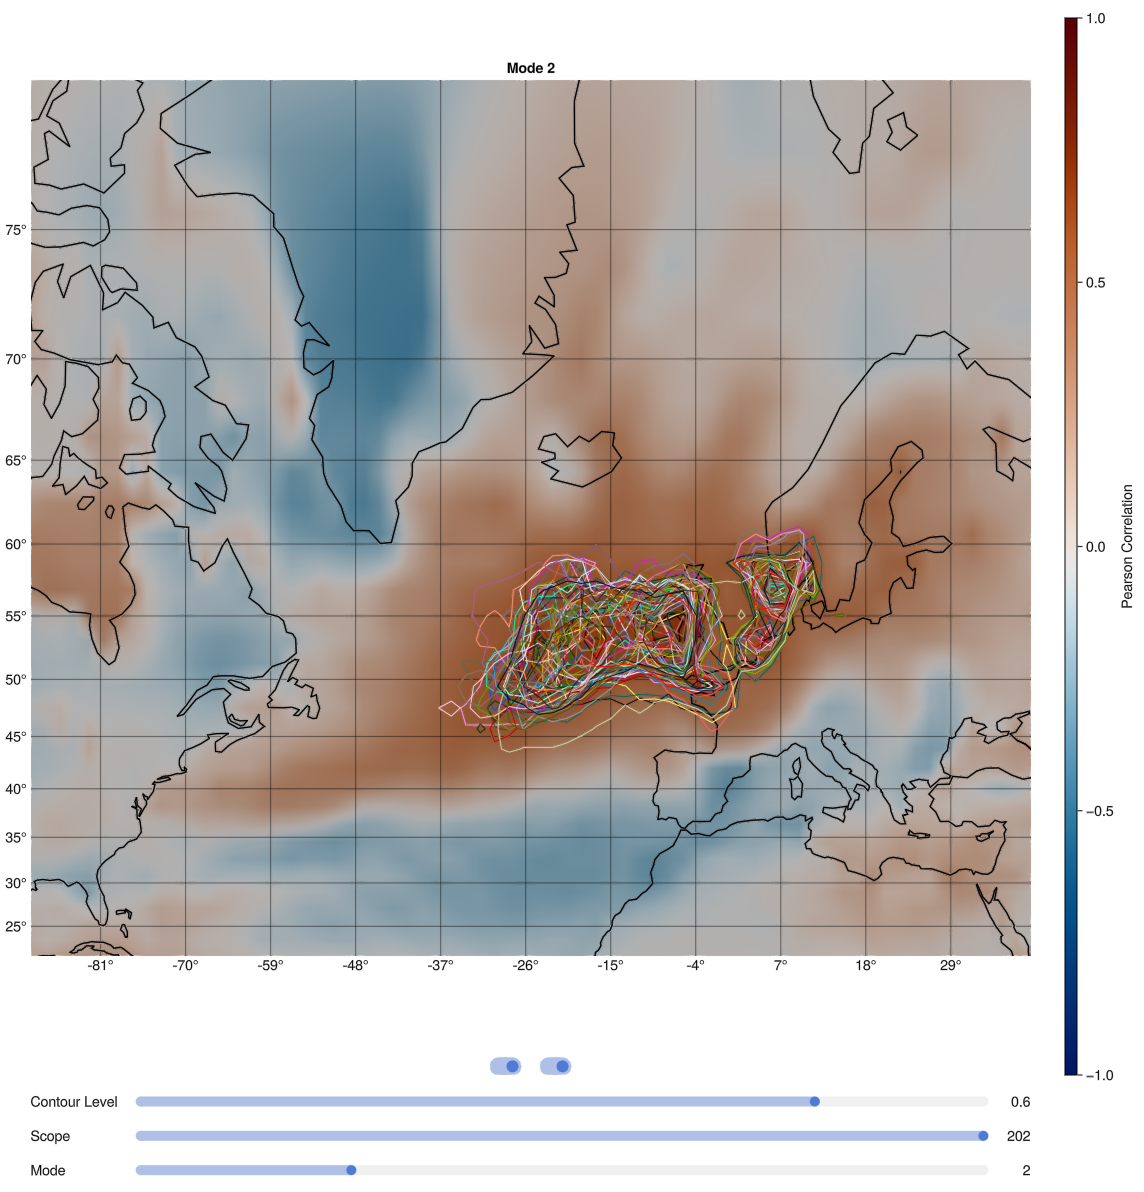
\includegraphics[width=\textwidth]{figures/ivt_pr_cor_mode2_ssp126.png}
    \caption{Spaghetti plots.}
    \label{fig:comparsion member vis spaghetti}
  \end{subfigure}
  \hfill
  \begin{subfigure}[b]{0.49\textwidth}
    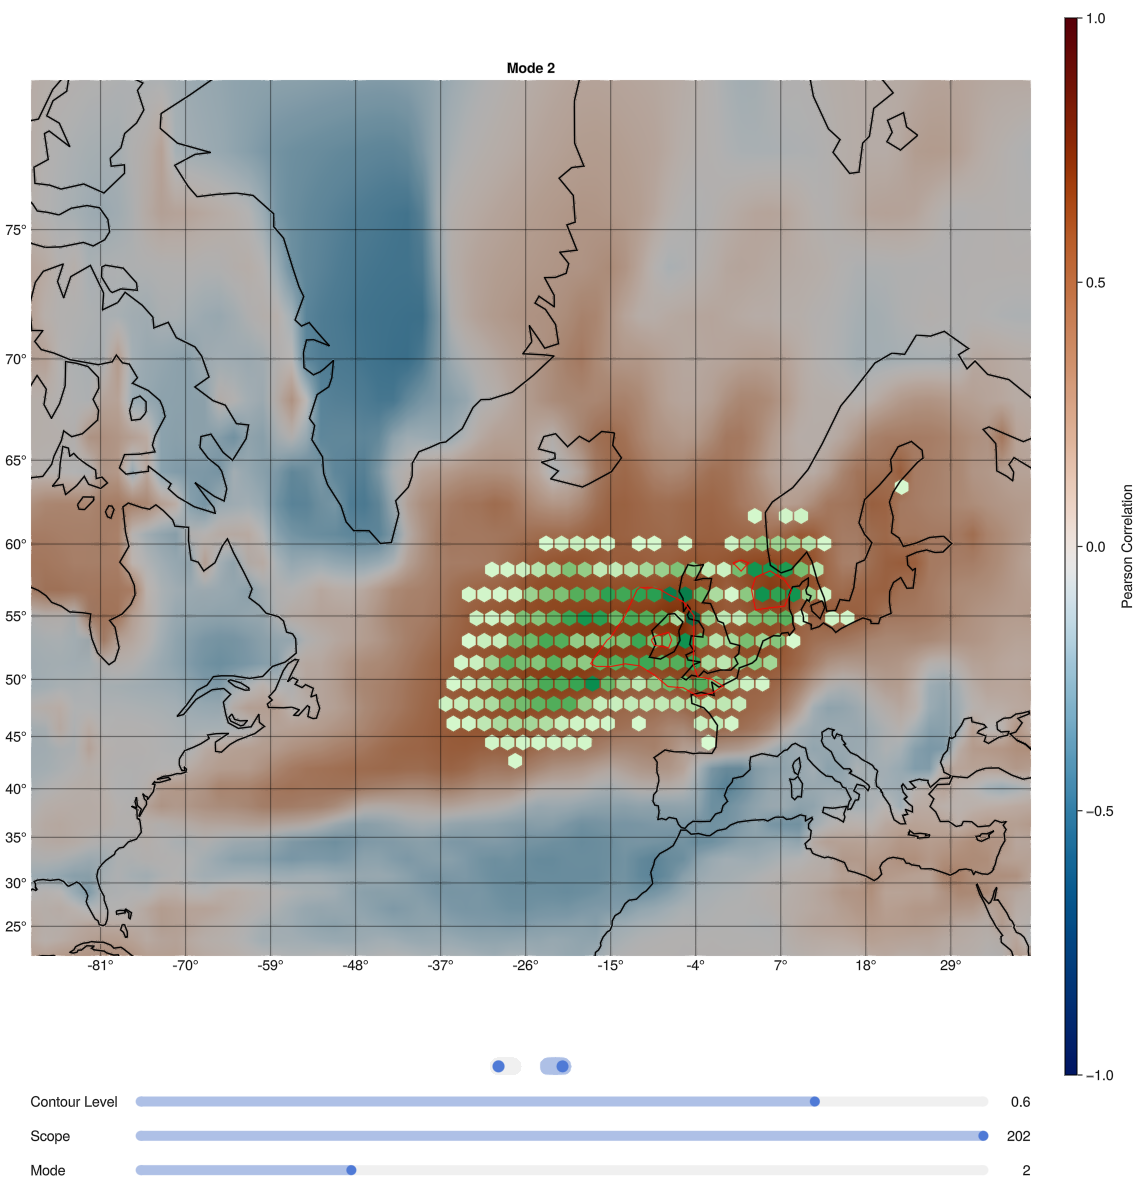
\includegraphics[width=\textwidth]{figures/ivt_pr_cor_mode2_ssp126_hexbin.png}
    \caption{Presented hexbin visualization}
    \label{fig:comparsion member vis hexbin}
  \end{subfigure}
  \caption{Comparison of spaghetti plots and the presented contour line visualization using hexbins. The picture is the SSP126 variant shown in Figure~\ref{fig:ivt eof pr cor mode2}.}
    \label{fig:comparsion member vis}
\end{figure}


The biggest waekness of the presented approach is the imprecision of the color of hexbins. 
Through the regression it is not entirely clear how many contour lines go through a bin. 
Additionally, the presented approach is susceptible for misrepresenting certain structers, e.g. a very small local high (of one member) of the size of one or two bins may make the impression of containing multiple members. 
A better way would be to implement it in a more stable way, each bin counting the exact amount of contour lines of diffenrent members passing through. 
But this would have required the implementation of a new Makie recipe\footnote{This is the name for cerain types of plots in Makie, like surface, heatmap or boxplot.}, which was out of scope for this Thesis. 

% \begin{itemize}
%   \item Goal was to improve on spaghetti plots and to reduce the chaos of them 
%   \item also it should give a hint on how coarse the actual, underlying data is 
%   \item did it work? Not really. It may look less chaotic for the cases where spaghetti plots also look not really that chaotic -> but for other cases its not that good 
%   \item also since its just a quick idea itis not really as precise as it could be (is based on a existing hexbin implementation rather than a newly written one)
%   \item also the resolution argument did not work for the slider since they somehow change size then
%   \item in the end: Best solution woiuld have been already existing ideas from recent papers -> but they provide no library (implementing a paper would have been out of scope for a master thesis beyond what I already did)
%
% \end{itemize}

